%!TEX encoding = UTF-8 Unicode
\documentclass[a4paper]{compendium}
\usepackage[swedish]{babel}
\addto\captionsswedish{%
  \renewcommand{\appendixname}{Appendix}%
}
%TODO: Glossary
%http://tex.stackexchange.com/questions/5821/creating-a-standalone-glossary/5837#5837

\setlength{\columnsep}{16mm}

\title{
{\vspace{-3.0cm}\bf\sffamily\Huge\selectfont  Introduktion till programmering med Scala och Java} 
\\ \vspace{1em}%\hspace*{1.5cm}\inputgraphics[width=0.6\textwidth]{../img/gurka} \\
{\sffamily  Grundkurs}\\\vspace{2cm}
%
\includegraphics[height=4cm]{../img/scala-logo.png}
%
\includegraphics[height=4cm]{../img/java-logo.png}

\includegraphics[height=12cm]{cover/gurka.jpg}
}

%\author{Redaktör: Björn Regnell}
\date{\raggedbottom%
\vspace{-2em}\begin{minipage}{1.0\textwidth}\centering
EDAA45, Lp1-2, HT 2016\\ 
Datavetenskap, LTH\\ 
Lunds Universitet\\
~\\
Kompileringsdatum: \today \\
\url{http://cs.lth.se/pgk} 
\end{minipage}
}

\usepackage{pgffor}  %% http://stackoverflow.com/questions/2561791/iteration-in-latex
                     %  allows:  \foreach \n in {1,...,4}{ do something with \n }

\usepackage{framed}  %  allows:   \begin{framed}\end{framed}
%\newenvironment{Slide}[2][]
%  {\begin{framed}\setlist{noitemsep}\section*{#2}}
%  {\end{framed}}

\newcommand{\SlideHeading}[1]{\section*{#1}}

\usepackage[most]{tcolorbox}
\newenvironment{Slide}[2][]
  {\vspace{0.5em}\begin{tcolorbox}[%width=1.05\textwidth,
  grow to right by=0.03\textwidth,grow to left by=0.03\textwidth,%breakable, 
                                   enhanced]\setlist{noitemsep}\SlideHeading{#2}}
  {\end{tcolorbox}\vspace{0.5em}}

\newcommand{\Subsection}[1]{} %ignore slide sections
\newcommand{\SlideOnly}[1]{} %ignore slide font size

\newif\ifkompendium  % to allow conditional text in slides only showing up in compendium
\kompendiumtrue      % in slides: \kompendiumfalse
                

%!TEX encoding = UTF-8 Unicode

\newcommand{\ModWeekONE}{Introduktion}
\newcommand{\ExeWeekONE}{expressions}
\newcommand{\LabWeekONE}{kojo}


\newcommand{\ModWeekTWO}{Program, kontrollstrukturer}
\newcommand{\ExeWeekTWO}{programs}
\newcommand{\LabWeekTWO}{--}


\newcommand{\ModWeekTHREE}{Funktioner, abstraktion}
\newcommand{\ExeWeekTHREE}{functions}
\newcommand{\LabWeekTHREE}{irritext}


\newcommand{\ModWeekFOUR}{Objekt, inkapsling}
\newcommand{\ExeWeekFOUR}{objects}
\newcommand{\LabWeekFOUR}{blockmole}


\newcommand{\ModWeekFIVE}{Klasser, datamodellering}
\newcommand{\ExeWeekFIVE}{classes}
\newcommand{\LabWeekFIVE}{--}


\newcommand{\ModWeekSIX}{Mönster, felhantering}
\newcommand{\ExeWeekSIX}{patterns}
\newcommand{\LabWeekSIX}{blockbattle}


\newcommand{\ModWeekSEVEN}{Sekvenser, enumerationer}
\newcommand{\ExeWeekSEVEN}{sequences}
\newcommand{\LabWeekSEVEN}{shuffle}


\newcommand{\ModWeekEIGHT}{Matriser, typparametrar}
\newcommand{\ExeWeekEIGHT}{matrices}
\newcommand{\LabWeekEIGHT}{life}


\newcommand{\ModWeekNINE}{Mängder, tabeller}
\newcommand{\ExeWeekNINE}{lookup}
\newcommand{\LabWeekNINE}{words}


\newcommand{\ModWeekTEN}{Arv, komposition}
\newcommand{\ExeWeekTEN}{inheritance}
\newcommand{\LabWeekTEN}{snake0}


\newcommand{\ModWeekELEVEN}{Kontextuella abstraktioner, api}
\newcommand{\ExeWeekELEVEN}{context}
\newcommand{\LabWeekELEVEN}{snake1}


\newcommand{\ModWeekTWELVE}{Valfri fördjupning, Projekt}
\newcommand{\ExeWeekTWELVE}{extra}
\newcommand{\LabWeekTWELVE}{Projekt0}


\newcommand{\ModWeekTHIRTEEN}{Repetition}
\newcommand{\ExeWeekTHIRTEEN}{examprep}
\newcommand{\LabWeekTHIRTEEN}{Projekt1}


\newcommand{\ModWeekFOURTEEN}{Muntligt prov}
\newcommand{\ExeWeekFOURTEEN}{Munta}
\newcommand{\LabWeekFOURTEEN}{Munta}


\begin{document}

\pagenumbering{roman}

\frontmatter
\maketitle
%!TEX encoding = UTF-8 Unicode
%!TEX root = ../compendium.tex

\clearpage\null\thispagestyle{empty}
\vfill

{
\setlength{\parindent}{0pt}
\emph{Editor}: Björn Regnell \\

%  LIST OF CONTRIBUTORS to https://github.com/lunduniversity/introprog
%    Please contact bjorn.regnell@cs.lth.se if you think you should be
%    on this list, or make a pull request with an update of file briefly
%    describing your contribtion in the commit text.
%    This work is licenced under CC-BY-SA-4.0.
%!TEX encoding = UTF-8 Unicode
%!TEX root = compendium/compendium.tex
\hyphenation{Borg-lund Da-ne-bjer Grampp Palm-qvist Ravn-borg Ro-sen-qvist Schrei-ter Wih-lan-der}
\emph{Contributors} in alphabetical order:
Anders Buhl,
André Philipsson Eriksson,
Anna Axelsson,
Anna Palmqvist Sjövall,
Anton Andersson,
Benjamin Lindberg,
Björn Regnell,
Casper Schreiter,
Cecilia Lindskog,
Dag Hemberg,
Elliot Bräck,
Elsa Cervetti Ogestad,
Emelie Engström,
Emil Wihlander,
Erik Bjäreholt,
Erik Grampp,
Evelyn Beck,
Fredrik Danebjer,
Gustav Cedersjö,
Henrik Olsson,
Hussein Taher,
Jakob Hök,
Jakob Sinclair,
Johan Ravnborg,
Jonas Danebjer,
Jos Rosenqvist,
Maj Stenmark,
Maria Kulesh,
Måns Magnusson,
Nicholas Boyd Isacsson,
Niklas Sandén,
Oliver Persson,
Oscar Sigurdsson,
Oskar Berg,
Oskar Widmark,
Patrik Persson,
Per Holm,
Philip Sadrian,
Sandra Nilsson,
Sebastian Hegardt,
Simon Persson,
Stefan Jonsson,
Theodor Lundqvist,
Tim Borglund,
Tom Postema,
Valthor Halldorsson,
Viktor Claesson,
Wilhelm Wanecek,
William Karlsson.

\\ \newline

\emph{Home}: \url{https://cs.lth.se/pgk} \newline

\emph{Repo}: \url{https://github.com/lunduniversity/introprog} \\ \newline

This compendium is on-going work. \\ \textbf{Contributions are welcome!} \\
\emph{Contact}: \url{bjorn.regnell@cs.lth.se}
\\ \newline

%\emph{Cover art}: Björn Regnell (inspired by Poul Ströyer's illustration of Lennart Hellsing's lyrics to  the childrens song ''Herr Gurka'' with music by Knut Brodin)\\ \newline

~\\ \newline

You can use this work if you respect this \emph{LICENCE}: CC BY-SA 4.0 \\
\url{http://creativecommons.org/licenses/by-sa/4.0/} \\
Please do \emph{not} distribute your solutions to lab assignments and projects.
\\ \newline
Copyright \copyright~ 2015-2017. \\
Dept. of Computer Science, LTH, Lund University. Lund. Sweden.\\
}

%!TEX encoding = UTF-8 Unicode
%!TEX root = ../compendium.tex

\ChapterUnnum{Framstegsprotokoll} 


\subsubsection*{Genomförda övningar}

\vspace{1em}\noindent 
{Till varje laboration hör en övning med uppgifter som utgör förberedelse inför labben. Du behöver minst behärska grundövningarna för att klara labben inom rimlig tid. Om du känner att du behöver öva mer på grunderna, gör då även extrauppgifterna. Om du vill fördjupa dig, gör fördjupningsuppgifterna som är på mer avancerad nivå. Kryssa för nedan vilka övningar du har gjort, så blir lätt för din handledare att se vilka kunskaper du förvärvat hittills.}

\newcommand{\TickBox}{\raisebox{-.50ex}{\Large$\square$}}
\newcommand{\ExeRow}[1]{\texttt{#1} & \TickBox  &  \TickBox &  \TickBox  \\ \addlinespace }

\begin{table}[h]
\centering
\vspace{2em}
\begin{tabular}{lccc}
\toprule \addlinespace 
{\sffamily\small Övning} & 
{\sffamily\small Grund} &	
{\sffamily\small Extra} &
{\sffamily\small Fördjupning}\\ \addlinespace \midrule \\[-0.7em]
\ExeRow{expressions}
\ExeRow{statements}
\ExeRow{functions}
\ExeRow{data}
\ExeRow{vectors}
\ExeRow{classes}
\ExeRow{traits}
\ExeRow{matching}
\ExeRow{matrices}
\ExeRow{sorting}
\ExeRow{scalajava}
\ExeRow{threads}
\bottomrule
\end{tabular}
\end{table}

\newpage

\subsubsection*{Godkända obligatoriska moment}

\vspace{1em}\noindent 
För att bli godkänd på laborationsuppgifterna och projektuppgiften måste du lösa deluppgifterna och diskutera dina lösningar med en handledare. Denna diskussion är din möjlighet att få feedback på dina lösningar. Ta vara på den!
Se till att handledaren noterar nedan när du blivit godkänd på respektive labb. Spara detta blad tills du fått slutbetyg i kursen. 


\vspace{2.5em}\noindent Namn: \dotfill\\

\vspace{1em}\noindent Namnteckning: \dotfill\\

\newcommand{\LabRow}[1]{\\[-1.1em] \texttt{#1} & \dotfill &  \dotfill  \\ \addlinespace }

\begin{table}[h]
\centering
\vspace{1em}
\begin{tabular}{lcc}
\toprule \addlinespace 
{\sffamily\bfseries\small Lab} & {\sffamily\small Datum gk} &	{\sffamily\small Handledares namnteckning}\\ \addlinespace \midrule \\[-0.5em]
%!TEX encoding = UTF-8 Unicode
%!TEX root = ../compendium2.tex
\LabRow{kojo}
\LabRow{irritext}
\LabRow{blockmole}
\LabRow{blockbattle}
\LabRow{shuffle}
\LabRow{words}
\LabRow{life}
\LabRow{snake}
\LabRow{music}
\LabRow{javatext}
\LabRow{survey}
%\toprule 
\addlinespace \midrule \addlinespace
 \\
{\sffamily\small {\bfseries Projektuppgift} (välj en)	} & \dotfill&\dotfill \\ \addlinespace\addlinespace %\midrule
\texttt{( ) bank}  &  &  \\
\texttt{( ) imageprocessing}  \\
\texttt{( ) tictactoe} \\  
\texttt{( ) }\textit{egendefinerad}  \\
\textit{\small Om egen, ge kort beskrivning:}\\
%\dotfill  \\
\bottomrule
\end{tabular}
\end{table}
%!TEX root = ../compendium.tex


\ChapterUnnum{Förord} 

Programmering är inte bara ett sätt att ta makten över systemen som styr vårt samhälle. Det är också ett kraftfullt verktyg för tanken. Att lära sig programmering och systemutveckling är första steget på en livslång resa av kontinuerligt lärande. Programmeringsspråk och utvecklingsverktyg kommer och går, men de grundläggande koncepten sekvens, alternativ, repetition och abstraktion som ligger bakom all mjukvara består. 

Detta kompendium utgör kursmaterial för studier i grundläggande programmering, med syfte att ge en solid bas för ingenjörsstudenter och andra som utvecklar system som innehåller mjukvara. 

Kompendiet är framtaget av, med och för studenter och lärare på universitetsnivå, och distribueras som öppen källkod. Det får användas fritt så länge erkännande ges och eventuella ändringar också publiceras som öppen källkod under samma licens som ursprungsmaterialet. På kursens hemsida \href{http://cs.lth.se/pgk}{cs.lth.se/pgk} och repo \href{http://github.com/lunduniversity/introprog}{github.com/lunduniversity/introprog} finns instruktioner om hur du kan bidra till kursmaterialet.

Läromaterialet fokuserar på lärande genom eget arbete och innehåller övningar och laborationer som är organiserade i moduler. Varje modul har ett tema och tillhörande föreläsningsanteckningar.

I kursen används språken Scala och Java för att illustrera grunderna i imperativ och objektorienterad programmering, tillsammans med elementär funktionsprogrammering. Mer avancerad objektorientering och funktionsprogrammering och  lämnas till fortsättningskurser. 



Den kanske viktigaste framgångsfaktorn vid studier i programmering är att bejaka din egen upptäckarglädje och experimentlusta. Det fantastiska med programmering är att dina egna intellektuella konstruktioner faktiskt \emph{gör} något som just \emph{du} har bestämt! Ta vara på det och prova dig fram genom att koda egna idéer -- det är kul när det funkar men minst lika lärorikt är felsökning, buggrättande och alla misslyckade försök som efter hårt arbete vänds till lyckade lösningar och bestående lärdomar. 

Välkommen i programmeringens fascinerande värld och hjärtligt lycka till med dina studier!




\setcounter{tocdepth}{2} % set headings level in table of contents
\tableofcontents
\mainmatter

\pagenumbering{arabic}

\part{Om kursen}      
%!TEX root = ../compendium.tex

\ChapterUnnum{Kursens arkitektur}
\begin{framed}
%\noindent\resizebox{\columnwidth}{!}{%
%!TEX encoding = UTF-8 Unicode
\begin{tabular}{l|l|l|l}
\textit{W} & \textit{Modul} & \textit{Övn} & \textit{Lab} \\ \hline \hline
W01 & Introduktion            & expressions & kojo            \\
W02 & Kodstrukturer           & programs    & --              \\
W03 & Funktioner, Objekt      & functions   & bugs            \\
W04 & Datastrukturer          & data        & pirates         \\
W05 & Sekvensalgoritmer       & sequences   & cards           \\
W06 & Klasser, Likhet         & classes     & turtlegraphics  \\
W07 & Arv, Gränssnitt         & traits      & turtlerace-team \\
KS  & KONTROLLSKRIVN.         & --          & --              \\
W08 & Mönster, Undantag       & matching    & chords-team     \\
W09 & Matriser, Typparametrar & matrices    & maze            \\
W10 & Sökning, Sortering      & sorting     & surveydata-team \\
W11 & Scala och Java          & scalajava   & lthopoly-team   \\
W12 & Trådar                  & threads     & life            \\
W13 & Design                  & Uppsamling  & Projekt         \\
W14 & Tentaträning            & Extenta     & --              \\
T   & TENTAMEN                & --          & --              \\
\end{tabular}

%}
\end{framed}

Kursen består av ett antal moduler med tillhörande teori, övningar och laborationer. Genom att göra övningarna bearbetar du teorin och förebereder dig inför laborationerna. När du klarar laborationen i varje modul är du redo att gå vidare till efterkommande modul.  

\newcommand{\Subsection}[1]{} %ignore slide sections

\newenvironment{Slide}[2][]
  {\begin{framed}\setlist{noitemsep}\section*{#2}}
  {\end{framed}}

\newif\ifkompendium
\kompendiumtrue

%!TEX root = ../lect-week01.tex

%%%%%%%%%%%%%%%%%%%%%%%%%%%%%%%%%%%%%%
\Subsection{Om denna kurs}

%%%
\begin{Slide}{Vad och hur?}
\begin{itemize}
\item \emph{Vad} ska du lära dig?
\begin{itemize}
\item Grundläggande principer för programmering\\ $\implies$Inga förkunskaper i programmering krävs!
\item Konstruktion av algoritmer
\item Tänka i abstraktioner
\item Flera olika angreppsätt: imperativ programmering, objektorientering, funktionsprogrammering
\item Programspråken Scala och Java
\item Utvecklingsverktyg (editor, kompilator, utvecklingsmiljö)
\item Implementera, testa, felsöka
\end{itemize}

\item \emph{Hur} ska du lära dig?
\begin{itemize}
\item Genom praktiskt eget arbete: \Emph{Lära genom att göra!}
\item Genom studier av kursens teori: \Emph{Skapa förståelse!}
\item Genom samarbete med dina kurskamrater: \Emph{Gå djupare!}
\end{itemize}
\end{itemize}
\end{Slide}


\ifkompendium
\subsection{hej}
Denna text hamnar bara i kompediet

Hejsan svejsan

\begin{itemize}
\item some item
\end{itemize}


\begin{Code}
hej kod
\end{Code}
\fi


\ifkompendium\else
\begin{Slide}{TESTSLAJD EJ I KOMPENDIUM}
\begin{itemize}
\item \emph{Hej} på dig
\item blablab
\item blabla
\end{itemize}
\begin{Code}
hej kod
\end{Code}
\end{Slide}
\fi


%%%%%%%%%%%%%%%%%%%%%%%%%%%%%%%%%%%%%%
\ifkompendium\else
\Subsection{Meddelande från \href{http://lth.se/code}{Code@LTH}} 
\fi

\begin{itemize}
\item item
\item item
\item item
\item item
\end{itemize}


%!TEX encoding = UTF-8 Unicode
%!TEX root = ../compendium.tex

\ChapterUnnum{Anvisningar}

\SectionUnnum{Samarbetsgrupper}
\subsection*{Samarbetskontrakt}
\subsection*{Grupplaborationer}
\subsection*{Samarbetsbonus}
\SectionUnnum{Föreläsningar}
\SectionUnnum{Övningar}
\SectionUnnum{Laborationer}
 
\begin{itemize}
\item TODO!!! Skriv om pennan och ögat och bocken
\item TODO!!! Skriv att om man inte gör föreberedelserna hinner man inte labben på 2h
\end{itemize}
\SectionUnnum{Resurstider}
\SectionUnnum{Kontrollskrivning}
\SectionUnnum{Tentamen}

%\renewcommand{\SlideHeading}[1]{\subsection{#1}}  %numbering sections in compendium slides

\part{Moduler}         
\foreach \n in {1,...,9}{%
  \input{modules/w0\n-chapter.tex} 
  \input{modules/w0\n-exercise.tex}
  \input{modules/w0\n-lab.tex}
}
\foreach \n in {10,...,12}{%
  \input{modules/w\n-chapter.tex} 
  \input{modules/w\n-exercise.tex}
  \input{modules/w\n-lab.tex}
}
%!TEX encoding = UTF-8 Unicode

%!TEX root = ../compendium.tex

%!TEX encoding = UTF-8 Unicode
\chapter{Repetition}\label{chapter:W13}
Begrepp som ingår i denna veckas studier:
\begin{itemize}[noitemsep,label={$\square$},leftmargin=*]
\item göra extenta
\item förbereda projektredovisning
\item skapa dokumentation med scaladoc och javadoc\end{itemize}

    
%!TEX encoding = UTF-8 Unicode
%!TEX root = ../compendium2.tex

\Assignment{bank}

\subsection{Fokus}
\begin{itemize}[nosep,label={$\square$},leftmargin=*]
\item Kunna implementera ett helt program efter given specifikation
\item Kunna sätta samman olika delar från olika moduler
\item Förstå hur Java-klasser kan användas i Scala
\item Förstå och bedöma när immutable/mutable såväl som var/val bör användas i större sammanhang
\item Kunna använda sig av kompanjonsobjekt
\item Kunna läsa och skriva till fil
\item Kunna söka i olika datastrukturer på olika sätt
\end{itemize}

\subsection{Bakgrund}

I detta projekt ska du skriva ett program som håller reda på bankkonton och kunder i en bank. Programmet ska utöver att hålla reda på bankens nuvarande tillstånd även föra historik över alla tillståndsändringar. Historiken ska vara så pass detaljerad att det nuvarande tillståndet kan återskapas genom att återuppspela alla ändringar som finns lagrade i historiken.

Programmet ska vara helt textbaserat, man ska alltså interagera med programmet via terminalen där en meny skrivs ut och input görs via tangentbordet.

Du ska skriva större delen av programmet själv, utan någon färdig kod. Programmet ska dock följa de specifikationer som ges i uppgiften, såväl som de objektorienterade principer du lärt dig i kursen.

\subsection{Krav}

Kraven för bankapplikationen återfinns här nedan. För att bli godkänd på denna uppgift måste samtliga krav uppfyllas:

\begin{itemize}
\item Programmet ska ha följande menyval:

\begin{itemize}
\item 1. Hitta konton för en viss kontoinnehavare med angivet ID.
\item 2. Söka efter kunder på (del av) namn.
\item 3. Sätta in pengar på ett konto.
\item 4. Ta ut pengar på ett konto.
\item 5. Överföra pengar mellan två olika konton.
\item 6. Skapa ett nytt konto.
\item 7. Ta bort ett befintligt konto.
\item 8. Skriv ut bankens alla konton, sorterade i bokstavsordning efter innehavare.
\item 9. Återställa banken till tillståndet den hade vid ett givet datum. För enkelhetens skull får du permanent kassera all historik som skapades efter det datum banken återställs till.
\item 10. Avsluta.
\end{itemize}

\item När något av följande sker ska programmet notera det i historiken:
\begin{itemize}
\item Pengar sätts in på ett konto.
\item Pengar tas ut från ett konto.
\item Pengar överförs mellan två konton.
\item Ett konto skapas.
\item Ett konto tas bort.
\end{itemize}
\item Historiken ska sparas både i minnet och i en fil.
\item Då programmet startas ska det läsa in historikfilen för att återskapa tillståndet som banken hade tidigare.
\item Allt som berör användargränssnittet (såsom utskrifter till terminalen och inläsning från terminalen) ska ske i \code{BankApplication} eller hjälpklasser till \code{BankApplication}, inte i någon annan av klasserna som specificeras i uppgiften.
\item Alla metoder och attribut ska ha lämpliga åtkomsträttigheter.
\item Valen av val/var och immutable/mutable måste vara lämpliga.
\item Din indata måste ge samma resultat som i exemplen i bilagan.
\item Rimlig felhantering ska finnas. Det är alltså önskvärt att programmet inte kraschar då man matar in felaktig input, utan istället säger till användaren att input är ogiltlig.
\item Programdesignen ska följa de specifikationer som är angivna nedan.
\item Det räcker med att banken ska kunna hantera heltal, men detta ska göras med klassen \code{BigInt}.
\item Klassen \code{BankAccount} ska generera ett unikt kontonummer för varje konto. Dessa ska återställas om bankens tillstånd återställs till ett tidigare datum, d.v.s. att om en återställning av banken tar bort ett konto så ska dess kontonummer återigen bli tillgängligt.
\end{itemize}

\subsection{Design}
Nedan följer specifikationerna för de olika klasserna bankapplikationen måste innehålla:

\begin{ScalaSpec}{Customer}
/**
 * Describes a customer of a bank with provided name and id.
 */
case class Customer(name: String, id: Long) = {
	override def toString(): String = ???
}
\end{ScalaSpec}


\begin{ScalaSpec}{BankAccount}
/**
 * Creates a new bank account for the customer provided.
 * The account is given a unique account number and initially
 * has a balance of 0 kr.
 */
class BankAccount(val holder: Customer) = {

  /**
   * Deposits the provided amount in this account.
   */
  def deposit(amount: Int): Unit = ???

  /**
   * Returns the balance of this account.
   */
  def getBalance: Int = ???

  /**
   * Withdraws the provided amount from this account,
   * if there is enough money in the account. Returns true
   * if the transaction was successful, otherwise false.
   */
  def withdraw(amount: Int): Boolean = ???
}
\end{ScalaSpec}


\begin{ScalaSpec}{Bank}
/**
 * Creates a new bank with no accounts and no history.
 */
class Bank() = {

 /**
   * Returns a list of every bank account in the bank.
   * The returned list is sorted in alphabetical order based
   * on customer name.
   */
  def getAllAccounts(): Vector[BankAccount] = ???

  /**
   * Returns the account holding the provided account number.
   */
  def findByNumber(accountNbr: Int): Optional[BankAccount] = ???

  /**
   * Returns a list of every account belonging to
   * the customer with the provided id.
   */
  def findAccountsForHolder(id: Long): Vector[BankAccount] = ???

  /**
   * Returns a list of all customers whose names match
   * the provided name pattern.
   */
  def findByName(namePattern: String): Vector[Customer] = ???

 /**
   * Executes an event in the bank.
   * Returns a string describing whether the
   * event was successful or failed.
   */
  def doEvent(event: BankEvent): String = ???

  /**
   * Resets the bank to the state it had at the provided date.
   * Returns a string describing whether the event was
   * successful or failed.
   */
  def returnToState(returnDate: Date): String = ???
}
\end{ScalaSpec}


Till din hjälp innehåller kursens workspace följande färdigskrivna klasser:
\begin{itemize}
\item \code{Date}, en enkel wrapper av \code{Java.time} som du ska använda för att representera tidsstämplar.
\item \code{BankEvent} med tillhörande subtyper, som du ska använda för att representera förändringar av bankens tillstånd.
\end{itemize}


\subsection{Tips}

\begin{itemize}
\item Det enda sättet att förändra tillståndet för en \code{Bank} ska vara (förutom att anropa \code{returnToState}) att anropa \code{doEvent} med en \code{BankEvent} som beskriver tillståndsförändringen. Vid en första anblick kan detta kan verka lite väl bökigt, men när ändringshistoriken ska implementeras kommer det vara till stor hjälp att det finns en \code{BankEvent} som representerar varje ändring.

\item För att skriva till fil på ett enkelt sätt kan man t.ex. använda sig av statiska metoder i klassen \code{Files} som finns tillgänglig i \code{java.nio.file}. För att undvika portabilitetsproblem kan man då använda sig av ett bestämt \code{Charset}, t.ex. \code{UTF_8}, som finns tillgänglig i \code{java.nio.charset.StandardCharsets.UTF_8}.

\item För att läsa ifrån en fil kan man t.ex. använda sig av \code{Source} som finns tillgänglig i \code{scala.io.Source}.

\item Var noggrann med att testerna klarar alla tänkbara fall, och tänk på att fler fall än dem som givits i exempel kan förekomma vid rättning.
\end{itemize}

\subsection{Obligatoriska uppgifter}

\Task Implementera klassen \code{Customer}.

\Task Implementera klassen \code{BankAccount}.

\Task Skapa singelobjektet \code{BankApplication}, som ska innehålla \code{main}-metoden. Det kan vara bra att innan man fortsätter se till att denna skriver ut menyn korrekt och kan ta input från tangentbordet som motsvarar de menyval som finns.

\Task Implementera klassen \code{Bank}.

\Subtask Implementera menyval 6 och 8. Testa noga.

\Subtask Implementera ändringshistoriken. Varje gång \code{doEvent} anropas ska dess \code{BankEvent}-argument läggas till i historiken tillsammans med det nuvarande datumet.

\Subtask Implementera alla andra menyval, förutom menyval 9. Testa de nya menyvalen noga efterhand som du implementerar dem, i synnerhet så att ändringshistoriken fungerar korrekt. Gör de utökningar du anser behövs.

\Task Implementera säkerhetskopiering av historiken.

\Subtask När en \code{BankEvent} läggs till i historiken ska den också skrivas till en historikfil omedelbart. Banken ska ej behöva avslutas för att utskriften ska hamna på fil, om så vore fallet kan information gå förlorad om banken kraschar.

I workspace-katalogen för denna projektuppgift finns en historikfil bifogad. För bekvämlighet finns ett utdrag av denna fil infogad nedanför. Inläsning och utskrift ska ske med dess format:\\~\\
2016 3 7 10 6 N 850127 Fredrik\newline
2016 3 7 10 28 D 1000 16500\newline
2016 3 9 10 52 W 1000 3900\newline
2016 3 9 11 8 N 900318 Casper\newline
2016 3 9 16 28 D 1001 6500\newline
2016 4 1 10 11 W 1001 1900\newline
2016 4 1 11 19 W 1001 2000\newline
2016 4 2 16 33 N 651002 Björn\newline
2016 4 2 16 46 D 1002 25000\newline
2016 4 3 10 11 T 1002 1000 4000\\~\\
Formen är alltså:\\~\\
\textbf{År  Månad  Dag  Timme  Minut  BankEventTag  Parametrar}
\\~\\
De olika klasserna av \code{BankEvent} representeras med följande bokstav:

\begin{itemize}
\item D - \code{Deposit}
\item W - \code{Withdraw}
\item T - \code{Transfer}
\item N - \code{NewAccount}
\item E - \code{DeleteAccount}
\end{itemize}

\Subtask När programmet startar ska det läsa in alla händelser från historikfilen och återuppspela dem en efter en. På så sätt kan bankens tillstånd återställas, fastän vi bara har sparat ändringshistoriken och inte själva tillståndet.

\Task Implementera menyval 9 genom att först nollställa bankens tillstånd och sedan återuppspela allt i historiken som hände före det givna datumet. Resten av historiken bör tas bort permanent, både i minnet och i historikfilen.


\subsection{Frivilliga extrauppgifter}

Gör först klart projektets obligatoriska delar. Därefter kan du, om du vill, utöka ditt program enligt följande.

\Task Skriv en eller flera av klasserna \code{Customer} och \code{BankAccount} i Java istället och använd dig av dessa i din Scala-kod.

\Task	Implementera ett nytt menyalternativ som skriver ut all kontohistorik för en given person. I historiken ska finnas typ av händelse med tillhörande parametrar, dåvarande saldo vid händelsen, såväl som datumet för händelsen.

\subsection{Exempel på körning av programmet}

Nedan visas möjliga exempel på körning av programmet. Data som matas in av användaren är markerad i fetstil.
Ditt program måste inte se identiskt ut, men den övergripande strukturen såväl som resultat av körningen ska vara densamma.
När det första exemplet börjar förutsätts det att banken inte har några konton.

Listan över val, som är markerad i kursiv stil i det första exemplet, är inte utskriven i senare exempel för att spara plats på pappret. Ditt program ska alltid skriva ut listan över val före användaren ska mata in ett val.

% This environment uses minipage to prevent column breaks from occurring in the middle of an example
\newenvironment{exampleblock}
	{\begin{minipage}{\columnwidth}
	 - - - - - - - - - - - - - - - - - - - - - - - - - - -\\}
	{\end{minipage}}

\begin{multicols}{2}
\noindent
\begin{exampleblock}
\textit{
1.   Hitta ett konto för en given kund\\
2.   Sök efter kunder på (del av) namn\\
3.   Sätt in pengar\\
4.   Ta ut pengar\\
5.   Överför pengar mellan konton\\
6.   Skapa nytt konto\\
7.   Radera existerande konto\\
8.   Skriv ut alla konton i banken\\
9.   Återställ banken till ett tidigare datum\\
10.  Avsluta\\
}
Val: \textbf{6}\\
Namn: \textbf{Adam Asson}\\
Id: \textbf{6707071234}\\
Nytt konto skapat med kontonummer: 1000\\
10:03:0 CET 14 / 5 - 2016\\
\end{exampleblock}
\begin{exampleblock}
Val: \textbf{1}\\
Id: \textbf{6707071234}\\
Konto 1000 (Adam Asson, id 6707071234) 0 kr\\
10:04:0 CET 14 / 5 - 2016\\
\end{exampleblock}
\begin{exampleblock}
Val: \textbf{6}\\
Namn: \textbf{Berit Besson}\\
Id: \textbf{8505255678}\\
Nytt konto skapat med kontonummer: 1001\\
10:12:0 CET 14 / 5 - 2016\\
\end{exampleblock}
\begin{exampleblock}
Val: \textbf{2}\\
Namn: \textbf{adam}\\
Adam Asson, id 6707071234\\
10:15:0 CET 14 / 5 - 2016\\
\end{exampleblock}
\begin{exampleblock}
Val: \textbf{8}\\
Konto 1000 (Adam Asson, id 6707071234) 0 kr\\
Konto 1001 (Berit Besson, id 8505255678) 0 kr\\
10:13:0 CET 14 / 5 - 2016\\
\end{exampleblock}
\begin{exampleblock}
Val: \textbf{6}\\
Namn: \textbf{Berit Besson}\\
Id: \textbf{8505255678}\\
Nytt konto skapat med kontonummer: 1002\\
13:56:0 CET 14 / 5 - 2016\\
\end{exampleblock}
\begin{exampleblock}
Val: \textbf{2}\\
Namn: \textbf{erit}\\
Berit Besson, id 8505255678\\
14:01:0 CET 14 / 5 - 2016\\
\end{exampleblock}
\begin{exampleblock}
Val: \textbf{3}\\
Kontonummer: \textbf{1000}\\
Summa: \textbf{5000}\\
Transaktionen lyckades.\\
14:36:0 CET 14 / 5 - 2016\\
\end{exampleblock}
\begin{exampleblock}
Val: \textbf{5}\\
Kontonummer att överföra ifrån: \textbf{1000}\\
Kontonummer att överföra till: \textbf{1001}\\
Summa: \textbf{1000}\\
Transaktionen lyckades.\\
14:37:0 CET 14 / 5 - 2016\\
\end{exampleblock}
\begin{exampleblock}
Val: \textbf{8}\\
Konto 1000 (Adam Asson, id 6707071234) 4000 kr\\
Konto 1001 (Berit Besson, id 8505255678) 1000 kr\\
Konto 1002 (Berit Besson, id 8505255678) 0 kr\\
14:52:0 CET 14 / 5 - 2016\\
\end{exampleblock}
\begin{exampleblock}
Val: \textbf{7}\\
Ange konto att radera: \textbf{1002}\\
Transaktionen lyckades.\\
14:01:0 CET 14 / 5 - 2016\\
\end{exampleblock}
\begin{exampleblock}
Val: \textbf{8}\\
Konto 1000 (Adam Asson, id 6707071234) 4000 kr\\
Konto 1001 (Berit Besson, id 8505255678) 1000 kr\\
14:01:0 CET 14 / 5 - 2016\\
\end{exampleblock}
\begin{exampleblock}
Val: \textbf{9}\\
Vilket datum vill du återställa banken till?\\
År: \textbf{2016}\\
Månad: \textbf{5}\\
Datum (dag): \textbf{9}\\
Timme: \textbf{18}\\
Minut: \textbf{10}\\
Banken återställd.\\
15:00:0 CET 14 / 5 - 2016\\
\end{exampleblock}
\begin{exampleblock}
Val: \textbf{8}\\
Konto 1002 (Björn, id 651002) 25900 kr\\
Konto 1001 (Casper, id 900318) 4600 kr\\
Konto 1003 (Eva, id 950908) 6300 kr\\
Konto 1000 (Fredrik, id 850127) 11800 kr\\
Konto 1004 (Kajsa, id 810722) 17000 kr\\
15:01:0 CET 14 / 5 - 2016\\
\end{exampleblock}
\begin{exampleblock}
Val: \textbf{3}\\
Kontonummer: \textbf{1005}\\
Summa: \textbf{5000}\\
Transaktionen misslyckades. Inget sådant konto hittades.\\
15:06:0 CET 14 / 5 - 2016\\
\end{exampleblock}

\end{multicols}

%!TEX encoding = UTF-8 Unicode
%!TEX root = ../compendium.tex

\Assignment{tictactoe}

\subsection{Obligatoriska uppgifter}

\Task En uppgift.

\Subtask En underuppgift.

\Subtask En underuppgift.

\subsection{Frivilliga extrauppgifter}

\Task En uppgift.

\Subtask En underuppgift.

\Subtask En underuppgift.
%!TEX encoding = UTF-8 Unicode
%!TEX root = ../compendium.tex

\Assignment{imageprocessing}

\subsection{Bakgrund}

En digital bild består av ett rutnät (en matris) av pixlar. Varje pixel har en färg, och om man har många pixlar flyter de samman för ögat så att de tillsammans skapar en bild.

Det finns olika system för hur man färgsätter de olika pixlarna. T.ex. så används CMYK-systemet (cyan, magenta, gul, svart) vid blandning av färg som ska tryckas på papper eller annat material. På en dator däremot används vanligtvis RGB-systemet. RGB-systemet har tre grundfärger: röd, grön och blå. Mättnaden av varje grundfärg anges av ett heltal som vi i fortsättningen förutsätter ligger i intervallet [0, 255]. 0 anger ”ingen färg” och 255 anger ”maximal färg”. Man kan därmed representera 256 × 256 × 256 = 16 777 216 olika färgnyanser. Man kan också representera gråskalor; det gör man med färger som har samma värde på alla tre grundfärgerna: (0, 0, 0) är helt svart, (255, 255, 255) är helt vitt.


\subsection{Uppgiften}
Du ska skriva ett program där du implementerar olika filter som ska manipulera en given bild på ett flertal olika sätt. Filterklasserna ska ärva från en abstrakt \code{ImageFilter}-klass som är skriven i Java. \code{ImageFilter}-klassen hittar du i cslib.

Följande beskriver \code{ImageFilter}-klassen.

\begin{JavaSpec}{abstract class ImageFilter}
/**
 * Skapar ett filterobjekt med ett givet namn.
 */
protected ImageFilter(String name);

/**
 * Tar reda på filtrets namn.
 */
public String getName();

/**
 * Filtrerar bilden i matrisen inPixels och returnerar
 * resultatet i en ny matris. Utnyttjar eventuellt 
 * värdet av paramValue
 */
public abstract Color[][] apply(Color[][] inPixels,
				 double paramValue);

/**
 * Berättar huruvida ett filter behöver ett parmetervärde eller inte
 * @return true ifall parametervärde behövs, annars false
 */
public abstract boolean needsParameter();

/**
 * Beräknar intensiteten hos alla pixlarna i pixels,
 * returnerar resultatet i en ny matris.
 */
protected short[][] computeIntensity(Color[][] pixels):

/**
 * Faltar punkten p[i][j] med faltningskärnan kernel.
 * 
 * @param p 		matris med talvärden
 * @param i 		radindex får den aktuella punkten
 * @param j 		kolonnindex får den aktuella punkten
 * @param kernel	faltningskärnan, en 3x3-matris
 * @param weight	summan av elementen i kernel
 * @return 		resultatet av faltningen
 */
protected short convolve(short[][] p, int i, int j, 
			short[][] kernel, int weight);
\end{JavaSpec}

Utöver filterklasserna ska du även skapa ett program där du kan välja ett variabelt antal filter och sedan applicera dessa på en bild. För att åstadkomma detta ska du implementera klasserna \code{FilterChooser}, som hanterar val av filter, och \code{FilterList} som representerar vilka filter som ska användas. Klasserna har följande specifikationer:

\begin{ScalaSpec}{FilterList}
class FilterList = ???

/** Adds a filter to the FilterList */
def addFilter(filter: ImageFilter): Unit = ???
  
/** Applies all the filters on the given Image and draws it in SimpleWindow */
def applyFilters(image: Image, sw: SimpleWindow): Unit = ???
\end{ScalaSpec}

\begin{ScalaSpec}{FilterChooser}
/** Creates a FilterChooser with all the available filters */
class FilterChooser(filters: Array[ImageFilter]) = ???
  
/** Shows which filters are available and lets the user choose filters
*   until an escape sequence has been given and returns a FilterList which
*   contain the chosen filters
*   Example: 
*   Tryck på 1 för Blått-filter
*   Tryck på 2 för Kontrast-filter
*   Tryck på 3 för Gauss-filter
*   Tryck på 4 för Sobel-filter
*   Tryck 42 om du inte vill ha fler filter
*/
def chooseFilters(): FilterList = ???
\end{ScalaSpec}

Till din hjälp får du en \code{Image}-klass som representerar en bild samt ett \code{ImageUI} som hjälper dig att ladda in en JPEG bild.

\begin{ScalaSpec}{Image}
class Image(val image: BufferedImage);

/** Returns a matrix of Color-objects that represents an image */
def getColorMatrix: Array[Array[Color]];

/** Updates the image in accordance with the given Color-matrix */
def updateImage(pixels: Array[Array[Color]]): Unit;
\end{ScalaSpec}


\Task \textbf{Blåfilter.} Skriv en klass \code{BlueFilter} som skapar en blå version av bilden. Det vill säga skapa ett filter där varje pixel bara innehåller den blå komponenten. Testa filtret genom att skapa ett \code{ImageProcessing}-object som ska innehålla en \code{main}-metod (\code{ImageProcessing} ska användas och utökas i senare uppgifter). Använd \code{ImageUI} för att välja en bild på följande sätt:
\begin{Code}
val im = new Image(ImageUI.getImage)
\end{Code}
Använd \code{SimpleWindow} samt \code{image} attributet från \code{Image}-objektet för att visa bilden. 

\Task \textbf{inverteringsfilter.} Skriv en klass \code{InvertFilter} som inverterar en bild dvs skapar en ''negativ'' kopia av bilden. Ljusa färger ska alltså bli mörka och mörka färger ska bli ljusa.
Fundera över vad som kan menas med en inverterad eller negativ kopia: de nya RGB-värdena är inte ett dividerat med de gamla värdena (då skulle de nya värdena kunna bli flyttal) och inte de gamla värdena med ombytt tecken (då skulle de nya värdena bli negativa).

\Task \textbf{Gråskalningsfilter.} Skriv en klass \code{GrayScaleFilter} som gör om bilden till en gråskalebild. Använd \code{ImageFilter}s \code{computeIntensity} metod för att bestämma vilken intensitet varje pixel ska ha. Om intensiteten i en pixel till exempel är 105 så ska ett nytt \code{Color}-objekt med värdena (105, 105, 105) skapas.

\Task \textbf{Krypteringsfilter.} Skriv en klass \code{XORCryptFilter} som krypterar bilden med xor-operatorn ˆ. Denna operator gör binär xor mellan bitarna i ett heltal. Exempelvis ger 8 ˆ 127 värdet 119. Om man gör xor igen med 127, alltså 119 ˆ 127, får man tillbaka värdet 8. Varje pixel krypteras genom att använda xor-operatorn med ursprungsvärdena för rött, grönt och blått tillsammans med ett slumpmässigt heltalsvärde som genereras av Scalas Random klass. Använd \code{paramValue} för att ge \code{Random}-objektet ett seed. På så sätt kan du återskapa bilden genom att applicera krypteringsfiltret igen, med samma \code{paramValue}, på den numera krypterade bilden.

\Task \textbf{Gaussfiltrer.} Gaussfiltrering är ett exempel på så kallad faltningsfiltrering. Filtreringen bygger på att man modifierar varje bildpunkt genom att titta på punkten och omgivande punkter. 

För detta utnyttjar man en så kallad faltningskärna K som är en liten kvadratisk heltalsmatris. Man placerar K över varje element i intensitetsmatrisen och multiplicerar varje element i K med motsvarande element i intensitetsmatrisen. Man summerar produkterna och dividerar summan med summan av elementen i K för att få det nya värdet på intensiteten i punkten. Divisionen med summan gör man för att de nya intensiteterna ska hamna i rätt intervall.

Exempel:

\begin{minipage}{5cm}
\begin{displaymath}
\mathit{intensity} = \left(
\begin{array}{ccccc}
5 & 4 & 2 & 8 & \ldots \\
4 & 3 & 4 & 9 & \ldots \\
9 & 8 & 7 & 7 & \ldots \\
8 & 6 & 6 & 5 & \ldots \\
\vdots & \vdots & \vdots & \vdots & \ddots
\end{array}
\right)
\end{displaymath}
\end{minipage}\hspace{2cm}
\begin{minipage}{5cm}
\begin{displaymath}
K = \left(
\begin{array}{ccc}
0 & 1 & 0 \\
1 & 4 & 1 \\
0 & 1 & 0
\end{array}
\right)
\end{displaymath}
\end{minipage}

Här är summan av elementen i $K$ $1+1+4+1+1 = 8$. För att räkna ut det nya värdet på intensiteten i punkten med index \code{(1)(1)} (det nuvarande värdet är 3) beräknar man:

\begin{displaymath}
\mathit{newintensity} = \frac{0 \cdot 5 + 1 \cdot 4 + 0 \cdot 2 + 1 \cdot 4 + 4 \cdot 3 + 1 \cdot 4 + 0 \cdot 9 + 1 \cdot 8 + 0 \cdot 7}{8} = \frac{32}{8} = 4
\end{displaymath}


Man fortsätter med att flytta K ett steg åt höger och beräknar på motsvarande sätt ett nytt värde för elementet med index \code{(1)(2)} (där det nuvarande värdet är 4 och det nya värdet blir 5). Därefter gör man på samma sätt för alla element utom för ”ramen” dvs elementen i matrisens ytterkanter.

Skriv en klass \code{GaussFilter}som implementerar denna algoritm. Varje färg ska behandlas separat. Gör på följande sätt:
\begin{enumerate}
	\item Bilda tre short-matriser och lagra pixlarnas red-, green- och blue-komponenter i matriserna.
	\item Utför faltningen av de tre komponenterna för varje element och lagra ett nytt \code{Color}-objekt i \code{outPixels} för varje punkt.
	\item Elementen i ramen behandlas inte, men i \code{outPixels} måste också dessa element få värden. Enklast är att flytta över dessa element oförändrade från \code{inPixels} till \code{outPixels}. Man kan också sätta dem till \code{Color.WHITE}, men då kommer den filtrerade bilden att se något mindre ut.
\end{enumerate}

Använd \code{ImageFilter}s \code{convolve}-metod för att utföra faltningen. Metoden behöver en faltningsmatris, \code{kernel}, som input och ska anropas med red-, green- och blue-matrisen. Faltningsmatrisen kan vara ett attribut i klassen och ska ha följande utseende:

\begin{displaymath}
\begin{pmatrix}
  0 & 1 & 0 \\
  1 & 4 & 1 \\
  0 & 1 & 0 \\
\end{pmatrix}
\end{displaymath}

Det kan vara intressant att prova med andra värden än 4 i mitten av faltningsmatrisen. Med värdet 0 får man en större utjämning eftersom man då inte alls tar hänsyn till den aktuella pixelns värde. Mata in detta värde i Parameter-rutan. 

Anmärkning: det kan ibland vara svårt att se någon skillnad mellan den filtrerade bilden och originalbilden. Om man vill ha en riktigt suddig bild så måste man använda en större matris som faltningskärna.


\Task  \textbf{Sobelfiltrer.} Sobelfiltrering är, precis som Gaussfiltrering, en typ av faltningsfiltrering. Med Sobelfiltrering får man dock motsatt effekt i jämförelse med Gaussfiltrering, dvs man förstärker konturer i en bild. I princip deriverar man bilden i x- och y-led och sammanställer resultatet.

\begin{figure}[H]
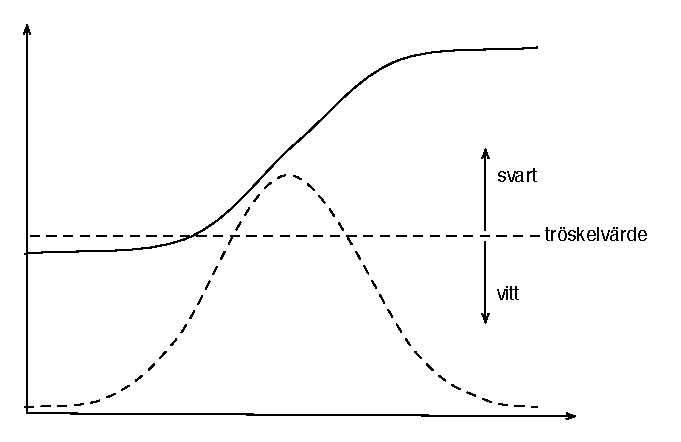
\includegraphics[width=\textwidth]{../img/w13-assignment-imageprocessing/derivatabild2.pdf}
\caption { En funktion (heldragen linje) och dess derivata (streckad linje).}
\label{fig:derivatabild}
\end{figure}

I figur~\ref{fig:derivatabild} visas en funktion $f$ (heldragen linje) och funktionens derivata $f'$ (streckad linje). Vi ser att där funktionen gör ett ''hopp'' så får derivatan ett stort värde. Om funktionen representerar intensiteten hos pixlarna längs en linje i x-led eller y-led så motsvarar ''hoppen'' en kontur i bilden. Om man sedan bestämmer sig för att pixlar där derivatans värde överstiger ett visst tröskelvärde ska vara svarta och andra pixlar vita så får man en bild med bara konturer. 

Nu är ju intensiteten hos pixlarna inte en kontinuerlig funktion som man kan derivera enligt vanliga matematiska regler. Men man kan approximera derivatan, till exempel med följande formel:

\begin{displaymath}
f'(x) \approx \frac{f(x+h) - f(x-h)}{2h}
\end{displaymath}

(Om man här låter $h$ gå mot noll så får man definitionen av derivatan.) Uttryckt i Scala och matrisen \code{intensity} så får man:

\begin{Code}
val derivative = (intensity(i)(j+1) - intensity(i)(j-1)) / 2
\end{Code}

Allt detta kan man uttrycka med hjälp av faltning. 

\begin{enumerate} 
	\item Beräkna intensitetsmatrisen med metoden \code{computeIntensity}.
	\item Falta varje punkt i intensitetsmatrisen med två kärnor:
$$
X\_SOBEL =
\begin{pmatrix}
  -1 & 0 & 1 \\
  -2 & 0 & 2 \\
  -1 & 0 & 1 \\
\end{pmatrix}
Y\_SOBEL =
\begin{pmatrix}
  -1 & -2 & -1 \\
  0 & 0 & 0 \\
  1 & 2 & 1 \\
\end{pmatrix}
$$
	Använd metoden \code{convolve} med vikten 1. Koefficienterna i matrisen $X\_SOBEL$ uttrycker derivering i x-led, i $Y\_SOBEL$ faltning i y-led. För att förklara varför koefficienterna ibland är 1 och ibland 2 måste man studera den bakomliggande teorin noggrant, men det gör vi inte här.
	\item Om resultaten av faltningen i en punkt betecknas med \code{sx} och \code{sy} så får man en indikator på närvaron av en kontur med \code{math.abs(sx) + math.abs(sy)}. Absolutbelopp behöver man eftersom man har negativa koefficienter i faltningsmatriserna. 
	\item  Sätt pixeln till svart om indikatorn är större än tröskelvärdet, till vit annars. Tröskelvärdet bestäms av \code{paramValue}. 
\end{enumerate}

Skriv en klass \code{SobelFilter} som implementerar denna algoritm.

\begin{figure}[H]
\begin{center}
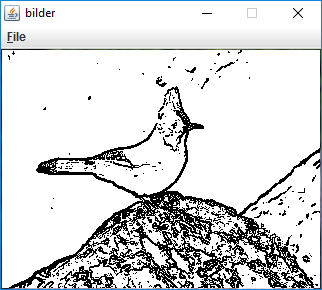
\includegraphics[scale=0.8]{../img/w13-assignment-imageprocessing/sobeljay.png}
\caption { Exempel på en bild där ett Sobelfilter applicerats med ett parametervärde på 150.}
\label{fig:sobel}
\end{center}
\end{figure}


\Task Implementera \code{FilterList} enligt specifikationerna ovan.

\Task Implementera \code{FilterChooser} enligt specifikationerna ovan.

\Task Knyt ihop allt i \code{ImageProcessing}-objektet som du skapade innan. Utskrifterna ska se ut på följande sätt:

{\setlength{\parindent}{0cm}

 Välj en av följande bilder genom att mata in en siffra\newline

0. boy.jpg\newline
1. car.jpg\newline
2. duck.jpg\newline
3. facade.jpg\newline
4. jay.jpg\newline
5. moon.jpg\newline
6. obidos.jpg\newline
7. sgrada.jpg\newline
8. shuttle.jpg\newline
Ditt val: 1\newline
Bild car.jpg laddad\newline
Tryck på 0 för Vanligt-filter\newline
Tryck på 1 för Blått-filter\newline
Tryck på 2 för Krypterat-filter\newline
Tryck på 3 för Inverterat-filter\newline
Tryck på 4 för Grått-filter\newline
Tryck på 5 för Kontrast-filter\newline
Tryck på 6 för Gauss-filter\newline
Tryck på 7 för Sobel-filter\newline
Tryck 42 om du inte vill använda fler filter\newline
Välj ett filter 1\newline
Välj ett filter 42\newline
Välja ny bild? (y/n) n\newline
}

Tänk på att användaren kan mata in otillåtna värden. Detta ska hanteras på lämpligt sätt.

\subsection{Frivilliga extrauppgifter}

\Task \textbf{Kontrastfilter.} Om man applicerar kontrastfiltrering på en färgbild så kommer bilden att konverteras till en gråskalebild. (Man kan naturligtvis förbättra kontrasten i en färgbild och få en färgbild som resultat. Då behandlar man de tre färgkanalerna var för sig.) Många bilder lider av alltför låg kontrast. Det beror på att bilden inte utnyttjar hela det tillgängliga området 0–255 för intensiteten. Man får en bild med bättre kontrast om man ''töjer ut'' intervallet enligt följande formel (lineär interpolation):

\begin{Code}
val newIntensity = 255 * (intensity - 45) / (225 - 45)
\end{Code}

Som synes kommer en punkt med intensiteten 45 att få den nya intensiteten 0 och en punkt med intensiteten 225 att få den nya intensiteten 255. Mellanliggande punkter sprids ut jämnt över intervallet \code{[0, 255]}. För punkter med en intensitet mindre än 45 sätter man den nya intensiteten till 0, för punkter med en intensitet större än 225 sätter man den nya intensiteten till 255. Vi kallar intervallet där de flesta pixlarna finns för \code{[lowCut, highCut]}. De punkter som har intensitet mindre än \code{lowCut} sätter man till 0, de som har intensitet större än \code{highCut} sätter man till 255. För de övriga punkterna interpolerar man med formeln ovan (45 ersätts med \code{lowCut}, 225 med \code{highCut}).

Det återstår nu att hitta lämpliga värden på \code{lowCut} och \code{highCut}. Detta är inte något som kan göras helt automatiskt, eftersom värdena beror på intensitetsfördelningen hos bildpunkterna. Man börjar med att beräkna bildens intensitetshistogram, dvs hur många punkter i bilden som har intensiteten 0, hur många som har intensiteten 1, . . . , till och med 255.

I de flesta bildbehandlingsprogram kan man sedan titta på histogrammet och interaktivt bestämma värdena på \code{lowCut} och \code{highCut}. Så ska vi dock inte göra här. I stället bestämmer vi oss för ett procenttal \code{cutOff} (som bestäms av \code{paramValue}) och beräknar \code{lowCut} så att \code{cutOff} procent av punkterna i bilden har en intensitet som är mindre än \code{lowCut} och \code{highCut} så att \code{cutOff} procent av punkterna har en intensitet som är större än \code{highCut}.

Exempel: antag att en bild innehåller 100 000 pixlar och att \code{cutOff} är 1.5. Beräkna bildens intensitetshistogram i en vektor
\begin{Code} 
val histogram = Array[Int](256)
\end{Code}

Beräkna \code{lowCut} så att \code{histogram(0)} + ... + \code{histogram(lowCut)} = 0.015 * 100000 (så nära det går att komma, det blir troligen inte exakt likhet). Beräkna \code{highCut} på liknande sätt.

Sammanfattning av algoritmen:
\begin{enumerate}
	\item Beräkna intensiteten hos alla punkterna i bilden, lagra dem i en \code{short}-matris. Använd den färdigskrivna metoden \code{computeIntensity}.
	\item Beräkna bildens intensitetshistogram.
	\item Parametervärdet \code{paramValue} är det värde som ska användas som \code{cutOff}.
	\item Beräkna \code{lowCut} och \code{highCut} enligt ovan.
	\item Beräkna den nya intensiteten för varje pixel enligt interpolationsformeln och lagra de nya pixlarna i \code{outPixels}.
\end{enumerate}
Skriv en klass \code{ContrastFilter} som implementerar algoritmen. I katalogen \emph{images} kan bilden \emph{moon.jpg} vara lämpliga att testa, eftersom den har låg kontrast. Anmärkning: om \code{cutOff} sätts = 0 så får man samma resultat av denna filtrering som man får av \code{GrayScaleFilter}. Detta kan man se genom att studera interpolationsformeln.

%!TEX encoding = UTF-8 Unicode

%!TEX root = ../compendium2.tex

%!TEX encoding = UTF-8 Unicode
\chapter{Muntlig examen}\label{chapter:W14}


%!TEX encoding = UTF-8 Unicode
%!TEX root = ../lect-week14.tex

%%%

\Subsection{Tentatips}
\begin{Slide}{Före tentan:}\SlideFontSmall
\begin{enumerate}
\item Repetera övningar och labbar i kompendiet. 
\item Läs igenom föreläsningsanteckningar.
\item Studera \Emph{snabbref} \Alert{mycket noga} så att du vet vad som är givet och var det står, så att du kan hitta det du behöver snabbt.
\item Skapa och \Emph{memorera} en personlig \Emph{checklista} med programmeringsfel du brukar göra, som även inkluderar småfel, så som glömda parenteser och semikolon, och annat som en kompilator/IDE normalt hittar.
\item Tänk igenom hur du ska disponera dina 5 timmar på tentan.
\item Gör den minst en extenta som om det vore \Alert{skarpt läge}: 
\begin{enumerate}\SlideFontTiny
\item Avsätt 5 ostörda timmar (stäng av telefon, dator etc).
\item Inga hjälpmedel. Bara snabbref.
\item Förbered dryck och tilltugg.
\end{enumerate}
\end{enumerate}
\end{Slide}

\begin{Slide}{På tentan:} \SlideFontTiny
\begin{enumerate}
\item Läs igenom \Alert{hela} tentan först. \\ \Emph{Varför?} Förstå helheten. Delarna hänger ihop.
\item Notera och begrunda specifika begrepp och definitioner. \\ \Emph{Varför?} Begreppen är avgörande för förståelsen av uppgiften.
\item Notera förenklingar, antaganden och specialfall. \\ \Emph{Varför?} Uppgiften blir mkt enklare om du inte behöver hantera dessa.
\item \Alert{Fråga} tentamensansvarig om du inte förstår uppgiften -- speciellt om det finns misstänkta felaktigheter eller förmodat oavsiktliga oklarheter. \\ \Emph{Varför?} Det är inte lätt att konstruera en ''perfekt'' tenta. \\ Du får fråga vad du vill, men det är inte säkert du får svar :)
\item Läs specifikationskommentarerna och metodsignaturerna i alla givna klass-specifikationer \Alert{mycket noga}. \\ \Emph{Varför?} Det är ett vanligt misstag att förbise de ledtrådar som ges där.
\item Återskapa din memorerade personliga checklista för vanliga fel som du brukar göra och avsätt tid till att gå igenom den på tentan. Varje fix plockar poäng!
\item Lämna in ett försök även om du vet att lösningen inte är fullständig. Det gäller att ''plocka poäng'' på så mycket som möjligt. En dålig lösning kan ändå ge poäng.

\item Om du har svårigheter kan det bli kamp mot klockan. Försök hålla huvudet kallt och prioritera utifrån var du kan plocka flest poäng. Ge inte upp! Ta en kort äta-dricka-paus för att få mer energi!

\end{enumerate}
\end{Slide}

\ifkompendium\else

\begin{Slide}{Planeringstips}\SlideFontTiny
Exempel på saker som du kan lägga in tid för i din julpluggkalender:
\begin{enumerate}
\item Välja ut övningar att repetera
\item Repetera övning X, Y, Z, ... Både läsa och skriva kod. Fundera på typ och värde.
\item Välja ut labbar att repetera
\item Repetera labb X, Y, Z, ... Lär dig ''trick'' och ''mönster''.
\item Träna på att skriva program med papper och penna
\item Göra checklista med vanliga fel
\item Läsa igenom extentor i Java
\item Välja ut minst en Java-extenta att göra som i skarpt läge i Scala
\item Gör Java-extentor X, Y, Z, ... implementera (delar) i Scala
\item Gör utvalda delar av extenta X, Y, Z, ... i Java
\end{enumerate}
\end{Slide}

\Subsection{Avgränsning}

\begin{Slide}{Tentans struktur}
\begin{itemize}
\item Del A 20\%:\\\Emph{Läsa uttryck} där du ska \Alert{ange typ och värde}
\begin{itemize}\SlideFontTiny
\item Du kommer att behöva skriva ner delsteg och variablers värden (minnet)
\item Testar förståelse av variabler, uttryck, samlingar, algoritmer, arv, etc.
\item Uppdaterad (mildare) regel om ''rättningströskel'': \\
Ur senaste compendium.pdf kapitel 0.8: \textit{Om du på del A erhåller färre poäng än vad som krävs för att nå upp till en bestämd ''rättningströskel'', kan din tentamen komma att underkännas utan att del B bedöms.}
\item Liknar kompendiets övningar; rimlig att lösa och dubbelkolla på 1h
\end{itemize}


\item Del B 80\%:\\\Emph{Skriva kod} som uppfyller \Alert{krav och designspecifikation}
\begin{itemize}\SlideFontTiny
\item Testar att du själv kan skapa kod med delar som samverkar
\item Testar förmåga att gå från indata-utdata till algoritm \\
 givet: ledtrådar, design, ev. skiss på lösning, ev. pseudokod etc.
\item Liknar kompendiets labbar; rimlig att lösa och dubbelkolla på 4h 
\end{itemize}

\end{itemize}
\end{Slide}



\begin{Slide}{Vad kommer på tentan? (1 av 3)}\SlideFontTiny
\hspace{-1em}\begin{minipage}{1.0\textwidth}
Allmänt: 
\begin{itemize}\SlideFontTiny
\item Begrepp som är ''fördjupning'' krävs ej på tentan (men ökar förståelse)
\item Ok om du väljer en enklare lösning med basala begrepp som fungerar bra, \\i stället för en kortare/elegantare/mer avancerad lösning
\item Dessa moduler ingår ej på tentan: ''Trådar, webb'', ''Design, api''
\end{itemize}

\vspace{1em}\begin{tabular}{l | l | l}
\textbf{Modul} & \textit{Ingår t.ex.}& \textit{Avgränsning} (ej krav; ok anv. om lämpl.)\\\hline
Introduktion & uttryck, aritmetik, slumptal, & kan ha nytta av deMorgan men ej krav\\
             & strängar, typer, Unit   & skriva egna \code|s"$x"| (men kunna läsa)  \\
             & skillnad mellan heltal \& flyttal & Float, Byte, Short\\
             & variabler, for, while, if & hex-literaler, backticks\\ 
\hline
Kodstrukturer & iterering, SWAP, SUM, MIN/MAX & import, paketnamn\\             
              & loopar, Range, sats vs uttryck & ok att välja vilken loop du tycker passar\\
              & namn, synlighet, skuggning & scaladoc, javadoc, jar \\        
\hline
Funtioner,    & definiera, anropa, parameter& skapa egen kontrollstruktur\\
objekt        & returtyp, namnarop, defaultarg & stegad funktion, rekursion\\        
              & punktnotation, objekt vs static & lazy val\\        
              & map/foreach med egen funktion & \\
              & anonyma funktioner (lambda)  & \\                              

\end{tabular}
\end{minipage}
\end{Slide}


\begin{Slide}{Vad kommer på tentan? (2 av 3)}\SlideFontTiny
\hspace{-2em}\begin{minipage}{1.0\textwidth}
\begin{tabular}{l | l | l}
\textbf{Modul} & \textit{Ingår t.ex.}& \textit{Avgränsning} (ej krav; ok anv. om lämpl.)\\\hline
Datastrukt. & attribut, medlem, metod, klass & isInstanceOf (anv. match istället) \\
            & tupler, Vector, Set, Map & List (oftast Vector istället)\\
            & Source.fromFile          & java.nio.file \\
\hline
Sekvensalg. &  skapa ny samling från befintlig &  \\      
            &  registrering, Scanner, ArrayBuffer & StringBuilder\\
            &  uppdatera Array, ArrayBuffer, Vector & \\
            &  slumptalsfrö, scala.util.Random  &  \\
\hline

Klasser     &  new, this, synlighet  & null \\
            &  inkapsling, accessregler, private  & private[this] \\
            &  klassparameter, fabriksmetod  & \\
            &  class vs case class    & \\
            &  referenslikhet vs innehållslikhet    & \\
            &  föränderlig vs oföränderlig klass & \\
\hline
Arv         &  bastyp, subtyp, trait, extends  & \\
            &  överskuggning,                  & inmixning, \\
            &  Any, AnyVal, AnyRef, Object     & Null, Nothing\\
            &  accessregler vid arv, protected & final\\
            &  abstract class, case object     & \\
            
\end{tabular}
\end{minipage}
\end{Slide}


\begin{Slide}{Vad kommer på tentan? (3 av 3)}\SlideFontTiny
\hspace{-2em}\begin{minipage}{1.0\textwidth}
\begin{tabular}{l | l | l}
\textbf{Modul} & \textit{Ingår t.ex.}& \textit{Avgränsning} (ej krav; ok anv. om lämpl.)\\\hline

Mönster     & match, Option, Try & try catch, unapply\\
            & flatten, sealed            & flatMap, partiella funktioner\\
            & enkel equals utan arv     & hashcode, fullständig equals   \\ 
            & wildcard-mönster  & variabelbindn. i mönster, sekvensmönster\\
\hline

Matriser,     & indexering i nästlade strukturer & \\
typparametrar & nästlad for-sats  & \\ 
              & matriser i Java med array  & \\
              & använda generiska strukturer & skapa generiska strukturer\\ 
\hline

Sök, sortera & linjärsökning, binärsökning & algoritmisk komplexitet\\
            & compareTo, strängjämförelse & Ordering, Ordered\\
            & insättningssortering & räcker kunna en valfri sortering \\
\hline


Scala/Java & översätta enkel Java/Scala & try catch i Java \\
           & implemenetera Java-klass     &  arv i Java med super vid konstr.\\
           & grundläggande syntaxskillnader & \\
           & ArrayList vs ArrayBuffer & java.util.\{List, Set\}\\
           & Autoboxing vid ArrayList<Integer> & \\
\multicolumn{3}{c}{OBS! Java-övningar finns även här och där i andra moduler}\\
\hline           
     
\end{tabular}
\end{minipage}
\end{Slide}


\Subsection{Tips vid val av lösningar}


\begin{Slide}{Tips om val av klass/trait}\SlideFontSmall
Ofta ger tentan en specifik design, men du kan ha stor nytta av egna abstraktioner, speciellt \Emph{lokala funktioner} för att göra enklare dellösningar!

\pause\vspace{1em}Om du skulle behöva samla både attribut och metoder utöver givan specifikationer:
Singelobjekt, case-klass, klass, trait eller abstrakt klass?
\begin{itemize}\SlideFontTiny
\item Använd \code{object} om du behöver samla metoder (och variabler) i en modul som bara finns i en upplaga. Du får lokal namnrymd och punktnotation på köpet.
\item Använd en \code{case class} om du har \Emph{oföränderlig data}. Du får då även innehållslikhet, möjlighet till mönstermatchning, etc. på köpet! 
\item Behöver du \Alert{föränderligt tillstånd} använd en vanlig \code{class}.\\ Det normala är att tillståndet (alla attribut) är \code{private} eller \code{protected} och att all uppdatering och avläsning av tillståndet sker indirekt genom metoder (getters/setters/...). 
\item Behöver du en abstrakt bastyp utan konstruktorparametrar använd en \code{trait}. \\(Du får inmixningsmöjlighet med \code{with} på köpet. Inmixning kommer ej på tenta.)
\item Behöver du en abstrakt bastyp med konstruktorparametrar använd en \code{abstract class}. (Går dock ej att använda vid inmixning med \code{with}.)
\end{itemize}
\end{Slide}


\begin{Slide}{Tips om hur man läser en specifikation}\SlideFontSmall
När du läser en specifikation av en klass, en trait, eller ett singelobjekt:
\begin{itemize}
\item Tänk igenom vilket ansvar olika delar av koden har
\item Vad håller klassen reda på? \\$\rightarrow$ Ledtrådar till attribut
\item Vad ska klassen göra/räkna ut? \\$\rightarrow$ Ledtrådar till metoder och deras algoritm
\item Vilka andra klasser har nytta av denna metod? \\$\rightarrow$ Ledtrådar till hur klasserna samverkar för att lösa uppgiften
\end{itemize}
Rita gärna en bild med ett specifikt exempel på vilken data som olika instanser håller reda på och fundera på hur data skapas/beräknas/förändras
\end{Slide}


\begin{Slide}{Tips om val av samling}\SlideFontSmall

Generellt: Det är ofta enklare med oföränderliga samlingar med oföränderliga element och skapa nya samlingar vid förändring. Men ibland blir det enklare om man har föränderliga samlingar.

\begin{itemize}
\item Behöver du hantera värden \code{x} av t.ex. typen String med \Emph{heltalsindex}?
\begin{itemize}\SlideFontTiny
\item Om du klarar dig utan förändring av innehållet:\\ \code{ val xs: Vector[String]}
\item Om du behöver ändra innehåll men \Alert{inte} antal element: \\ \code{ val xs: Array[String]} 
\item Om du behöver ändra innehåll \Alert{och} antal element: 
\\ \code{ var xs: Vector[String] } (se metoden \code{patch}) eller \\ \code{ val xs: ArrayBuffer[String]} (har metoden \code{insert})
\end{itemize}

\item Behöver du hantera värden \code{x} som ska vara unika?
\begin{itemize}\SlideFontTiny
\item Oföränderlig: \code{  val xs: Set[String] }
\item Förändringsbar: \code{val xs: scala.collection.mutable.Set[String]}
\end{itemize}

\item Behöver du leta upp värden \code{x:Int} utifrån en nyckel av t.ex. String?
\begin{itemize}\SlideFontTiny
\item Oföränderlig: \code{   val xs: Map[String, Int] }
\item Förändringsbar: \code{val xs: scala.collection.mutable.Map[String, Int]}
\end{itemize}


\end{itemize}
\end{Slide}

\begin{Slide}{Tillåtna uppdateringar i din QuickRef}
Du får med egen penna göra dessa fixar i din QuickRef:
\begin{itemize}
\item Grundtypernas implementation, sid 4: 
\begin{itemize}

\item omfång för Int ska ha exponent 31 (inte 15), 
\item omfång för Long ska ha exponent 63 (inte 15).
\end{itemize}

\item Saknade samlingsmetoder: 
\begin{itemize}
\item Under rubriken "Methods in trait Map[K, V]" saknas metoderna keySet och mapValues. 
\item Saknade metoderna för mutable.ArrayBuffer[T]: \\ \code{update} \code{insert} \code{remove} \code{append} \code{prepend}, etc. \\ lägg till beskrivning på lediga platsen på sista sidan \\ 
(se vidare commit \href{https://github.com/lunduniversity/introprog/commit/a5e29d000062}{a5e29d000062a} i kursrepot)
\end{itemize}
\end{itemize}
\end{Slide}


\begin{Slide}{ArrayBuffer}
Viktigast att känna till: update, insert, remove, append
{\SlideFontTiny

\vspace{2.5em}\begin{tabular}{@{}p{4.2cm}  p{6.5cm}}
\texttt{xs(i) = x \newline xs.update(i, x)} & Replace element at index i with x. \newline Return type Unit.\\   \cline{1-2}

\texttt{xs.insert(i, x)\newline xs.remove(i)} & Insert x at index \texttt{i}. Remove element at i. \newline Return type Unit.\\   \cline{1-2}

\texttt{xs.append(x)~~~xs~+=~x} & Insert x at end.  Return type Unit.\\   \cline{1-2}

\texttt{xs.prepend(x)~~x~+=:~xs} & Insert x in front.  Return type Unit.\\   \cline{1-2}

\texttt{xs -= x} & Remove first occurance of x (if exists). \newline Returns xs itself. \\\cline{1-2}

\texttt{xs ++= ys} & Appends all elements in ys to xs and returns xs itself. \\

\end{tabular}
}
\end{Slide}



\Subsection{Genomgång av extenta}
\begin{Slide}{Extenta 2016-08-24 TimePlanner}\SlideFontSmall
\url{http://cs.lth.se/pgk/examination/}

\vspace{1em}\Alert{TimePlanner}: 
\begin{itemize}
\item \href{http://fileadmin.cs.lth.se/cs//Education/grundkurs/extentor/160824.pdf}{tentamen 160824} 
\item \href{http://fileadmin.cs.lth.se/cs//Education/grundkurs/extentor/sol-160824.pdf}{lösningsförslag Java} 
\item \href{https://github.com/lunduniversity/introprog/tree/master/compendium/examples/exam/re-impl-java-exams/timeplanner-160824}{översättning av lösning till Scala}
\end{itemize}
\end{Slide}


\Subsection{Avslutning av kursen}

\begin{Slide}{Obligatoriska moment}\SlideFontSmall
\begin{itemize}
\item Kolla vilka oblikatoriska moment du har kvar här:
\url{http://fileadmin.cs.lth.se/pgk/SAM-EDAA45-snapshot.html}
\item Sök på din födelsemånad/dag, tex 0102 för andra Januari.
\item Läs \Alert{alla} instruktioner \Alert{noga} och \Alert{anmäl dig} här: \\
\href{http://www.student.lth.se/studieinformation/anonyma-tentor/}{www.student.lth.se/studieinformation/anonyma-tentor}
\item Du ska vara godkänd på alla labbar+projekt för att få tenta pgk EDAA45!
\item Du ska vara godkänd på alla labbar+projekt för att få gå pfk \href{http://cs.lth.se/edaa01vt}{EDAA01}!
\item Använd återstående \Emph{resurstider} för \Alert{redovisning av labbar/projekt}.
\end{itemize}
\end{Slide}

\begin{Slide}{CEQ -- Course Experience Questionnaire}\SlideFontSmall
\begin{itemize}
\item Görs på hela LTH på samma sätt. Alla får länkar via mejl.
\item Snälla fyll i CEQ! Jag är \Alert{mycket tacksam} för all konstruktiv feedback! \\ Hög svarsfrekvens är viktigt för att kunna dra slutsatser om variationen i svaren och signifikansen i sammanställningen.
\item Del 1: Generella påståenden, alla med 5-gradig skala: \\ tar helt avstånd ... instämmer helt
\item Del 2: \Emph{Fritextfrågor}: \\
''Vad  tycker  du  var  det  bästa  med  den här  kursen?'' \\
''Vad  tycker  du  främst  behöver  förbättras?''
\item Fördel med CEQ: Samma alla kurser alla år medger jämförelse över tid.
\item Begränsning med CEQ: Saknar frågor kopplat till specifika kursmoment.
\item Mer om CEQ här: \url{https://www.ceq.lth.se/}
\end{itemize}
\end{Slide}

\begin{Slide}{Kursspecifik utvärdering om specifika kursmoment}\SlideFontSmall
\begin{itemize}
\item Jag vill gärna att alla gör den LTH-gemensamma, anonyma kursutvärderingsenkäten \href{https://www.ceq.lth.se/}{CEQ}. Dina fritext-kommentarer om vad som är det bästa med kursen och vad som främst behöver förbättra emottages mycket tacksamt i CEQ-utvärderingen!
\item Jag kommer att komplettera CEQ med en \Emph{kursspecifik} utvärdering av specifika kursmoment i denna kurs och jag är därför \Alert{mycket tacksam} om alla fyller enkäten när länk kommer via mejl. 
\item Jag behandlar dina svar konfidentiellt, men ber om din STiL-id så att jag kan återkomma om jag mot förmodan undrar något mer.
\item Din input är mycket värdefull vid framtida kursutveckling!
\end{itemize}
\end{Slide}

\begin{Slide}{Intresserad av att arbeta som handledare?}
\begin{itemize}
\item Vi har ständigt behov av nya handledare i våra kurser
\item Det är lärorikt att jobba som timanställd handledare
\item Kontakta \verb|bjorn.regnell@cs.lth.se| eller annan kursansvarig i den kurs du vill jobba
\end{itemize}
\end{Slide}

\begin{Slide}{Utblick}\SlideFontSmall
Några framtida \Emph{kurser} som direkt bygger på pgk:
\begin{itemize}
\item Fördjupningskursen (Java)
\item Utvärdering av programvarusystem (R)
\item Diskreta strukturer (Clojure)
\item Programvaruutveckling i grupp 
\item Objekt-orienterad modellering och design
\item Funktionsprogrammering 
\end{itemize}
Framtiden för \Emph{Scala}:
\begin{itemize}
\item Scala 2.12 bättre bytekod, Scala 2.13 bättre standardbibliotek
\item Ny kompilator: \Emph{dotty}; Nytt format ''över'' bytekod: \Emph{Tasty}
\item Scala.JS: dela kod+kompetens mellan backend och frontend
\item Scala native: kör Scala kompilerat direkt ''på metallen''
\item Scala-ramverk för stordata, massiv parallellism, AI, ...
\end{itemize}
\end{Slide}

\begin{Slide}{Hoppas att kursen varit kul och lärorik!}

\includegraphics[width=5cm]{../img/gurka.jpg}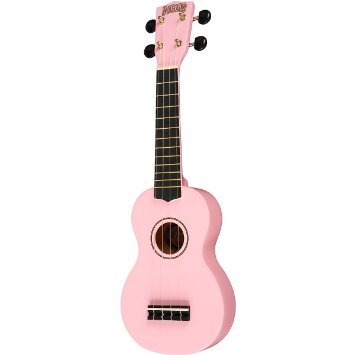
\includegraphics[width=5cm]{../img/ukulele.jpg}
\end{Slide}

\begin{Slide}{Ett stort TACK för...}
\begin{itemize}
\item ... att ni kämpat så hårt!
\item ... att ni ställt massor med frågor!
\item ... att det har varit så hög närvaro på föreläsningarna!
\item ... att ni är så konstruktiva och verkligen vill lära er!
\end{itemize}
\vspace{2em} \pause

\Alert{Ett stort LYCKA TILL på vägen till att bli en \\ kompetent och innovativ systemutvecklare!}
\end{Slide}


\fi
 


\part{Appendix}         
\appendix
%!TEX encoding = UTF-8 Unicode
%!TEX root = ../compendium2.tex

\chapter{Terminalfönster}\label{appendix:terminal}

\section{Vad är ett terminalfönster?}

I ett terminalfönster kan man skriva kommandon som kör program och hanterar filer. När man programmerar använder man ofta terminalkommando för att kompilera och exekvera sina program.  
 
\subsubsection{Terminal i Linux}

    \begin{figure}[!b]
    \centering
    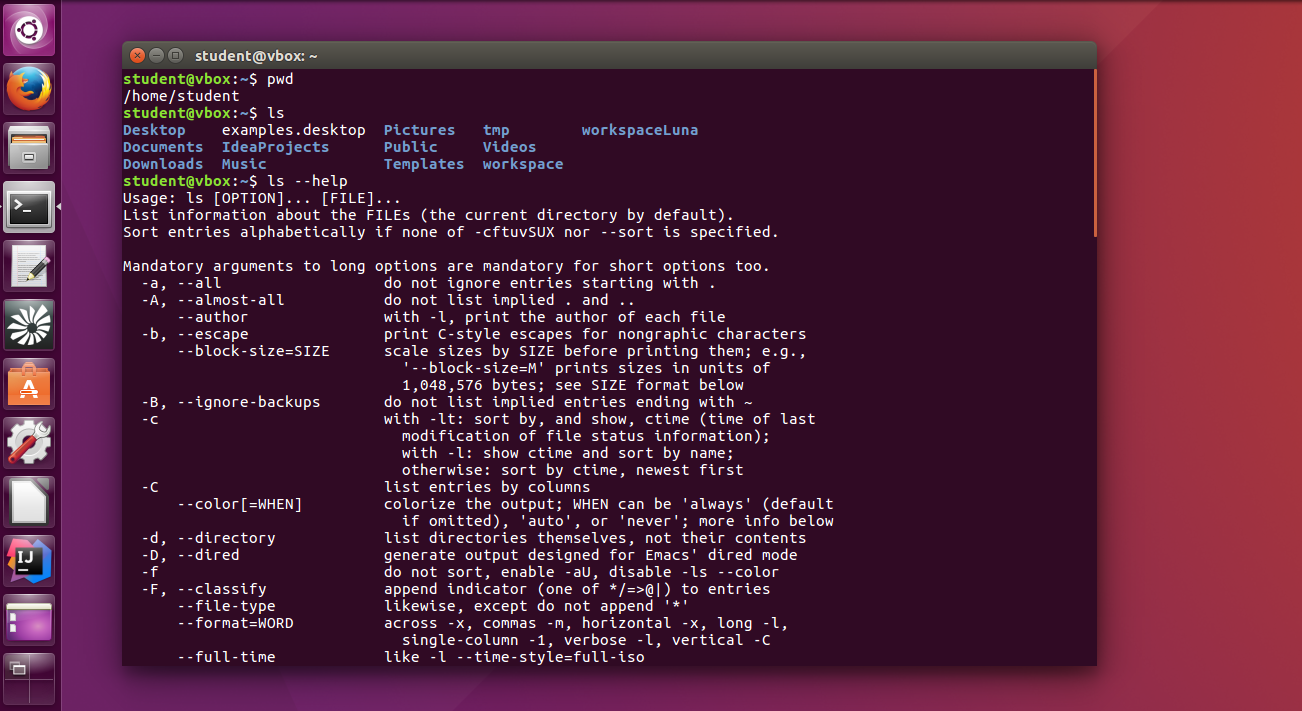
\includegraphics[width=1.0\textwidth]{../img/linux-terminal.png}
    \caption{Terminalfönster i Ubuntu öppnas med Ctrl+Alt+T.}
    \label{fig:terminal:linux}
    \end{figure}

I Ubuntu trycker du lättast \textbf{Ctrl+Alt+T} eller sök efter ''terminal'' i app-menyn.  Då öppnas ett fönster med en blinkande markör som visar att det är redo att ta emot dina textkommando. Ett exempel på kommando är \texttt{ls} som skriver ut en lista med filer i det aktuella biblioteket, så som visas i fig. \ref{fig:terminal:linux}.

Det som visas i ett terminalfönster sköts av ett \textbf{kommandoskal} \Eng{command shell}, som är redo att ta emot kommando efter en prompt som slutar med ett \texttt{\$}-tecken. När du skriver ett kommando och trycker Enter anropar kommandoskalet en kommandotolk som tolkar och utför dina kommandon. Om ett kommando inte kan tolkas, skrivs ett felmeddelande. 

Det finns många användbara kortkommando, varav de viktigaste visas i tabell \ref{fig:terminal:shortcuts}. Det är bra om du lär dig dessa kortkommandon utantill så att ditt arbete i terminalen går snabbt och smidigt.

\begin{table}[H]
\renewcommand{\arraystretch}{1.15}
\begin{tabular}{@{}r | l}
pil upp/ner & bläddra i kommandohistoriken \\
Tab & ''auto-complete'', fyll i resten baserat på vad du skrivit hittills \\
Tab Tab & två tryck på Tab listar flera alternativ, om så finnes \\
Ctrl+A & ''ahead'', flytta markören till början av raden \\
Ctrl+E & ''end'', flytta markören till slutet av raden \\
Ctrl+K & ''kill'', ta bort tecken från markören till radens slut\\
Ctrl+U & ''undo'', ta bort tecken från markören till början av raden \\
Ctrl+Y & ''yank'', sätt in det som senast togs bort\\
Ctrl+Z & ''zleep'', stoppa pågående process, skriv sedan \texttt{bg} för bakgrundskörning\\
Ctrl+L & rensa terminalfönstret\\
Ctrl+D & avsluta kommandoskalet \\
\end{tabular}
    \caption{Viktiga kortkommandon i Linux terminalfönster.}
    \label{fig:terminal:shortcuts}
\end{table}

\noindent Ctrl+C orsakar normalt ett avbrott av pågående process, men om du vill att Ctrl+C ska vara ''Copy'' som vanligt för att kopiera markerad text, kan du ställa om detta med terminalförnstrets  meny ''Edit $\rightarrow$ Keyboard Shortcuts'', eller liknande.




 
\subsubsection{PowerShell, Cmd och Linux i Microsoft Windows}
Microsoft Windows är inte Linux-baserat, men i kommandotolken \textbf{Powershell} finns alias definierade för några vanliga Linux-kommandon, inkluderat \texttt{ls}, \texttt{cd} och \texttt{pwd}. 
Du startar Powershell t.ex. genom att trycka på Windows-knappen och skriva \texttt{powershell}. 
Du kan också, medan du bläddrar bland filer, klicka på filnamnsraden överst i filbläddraren och skriva \texttt{powershell} och tryck Enter; då startas Powershell i aktuellt bibliotek. Ändra gärna typsnitt och bakgrundsfärg med hjälp av fönstrets menyer, så att det blir lättare för dig att läsa vad som skrivs.

Det finns även i Windows den ursprungliga kommandotolken \textbf{Cmd} med helt andra kommandon. Till exempel skriver man i Cmd kommandot \texttt{dir} i stället för \texttt{ls} för att lista filer. 

I Windows 10 kan du (numera, om du installerad senaste uppdateringarna av Windows) även köra Ubuntu-terminalen med hjälp av Windows Linux Subsystem (WSL). Se vidare här om hur du kan installera WSL under Windows 10: 

\url{https://ubuntu.com/wsl} 

Läs mer här: \href{https://www.omgubuntu.co.uk/2020/03/windows-10-linux-kernel-update}{www.omgubuntu.co.uk/2020/03/windows-10-linux-kernel-update}



\subsubsection{Terminal i Apple macOS/OS X}


Apple OS X och macOS är Unix-baserade operativsystem. De flesta vanliga terminalkommandon som fungerar i Linux fungerar också under Apple OS X och macOS. Du startar ett terminalfönster i Apples operativsystem genom att klicka på förstoringsglaset uppe till höger, skriva \texttt{terminal}, och trycka Enter.

\section{Vad är en path/sökväg?}\label{terminal:path}

När du skriver ett kommando i terminalen, eller kör vilket program som helst på din dator, behöver operativsystemet identifera i vilken fil programmets maskinkod ligger innan programmet kan köras. 

Lokaliseringen av filer sker med hjälp av en \textbf{sökväg} \Eng{path}, som anger en position i filsystemet. Ofta betraktas filsystemet som ett upp-och-ned-vänt träd, och kallas därför även ''filträdet''. Den ''översta'' positionen kallas ''rot'' \Eng{root} och betecknas med ett enkelt snedstreck \texttt{/}. Kataloger som ligger i kataloger utgör förgreningar i trädet. En sökväg pekar ut vägar genom trädet som behövs för att nå ''löven'', som utgörs av själva filerna.

Du kan se var ett program ligger i Linux med hjälp av kommandot \texttt{which} enligt nedan.\footnote{Skriv \texttt{ gcm ls } i Windows Powershell för motsvarighet till \texttt{ which ls } \\ Eller skriv \texttt{ New-Alias which get-command } för tillgång till kommandot \texttt{which} i Powershell. \\ \href{http://stackoverflow.com/questions/63805/equivalent-of-nix-which-command-in-powershell}{stackoverflow.com/questions/63805/equivalent-of-nix-which-command-in-powershell}} Listan med bibliotek i sökvägen avskiljs med snedstreck.
\begin{REPLnonum}
$ which java
/usr/lib/jvm/oracle_jdk8/bin/java
$ which ls
/bin/ls
\end{REPLnonum}

En sökväg kan vara \textbf{absolut} eller \textbf{relativ}. En absolut sökväg utgår från roten och visar hela vägen från rot till destination, t.ex. \texttt{/usr/bin/firefox}, medan en relativ sökväg utgår från aktuellt bibliotek (där du ''står'') och börjar \textit{inte} med ett snedstreck.

Alla operativsystem håller reda på en mängd olika sökvägar för att kunna hitta speciella filer i filträdet. Dessa sökvägar lagras i s.k. \textbf{miljövariabler} \Eng{environment variables}. Det finns en \textit{speciell} miljövariabel som heter kort och gott \textbf{PATH}, i vilken alla sökvägar till de program finns, som ska vara tillgängliga för din användaridentitet direkt för exekvering genom sina filnamn, \textit{utan} att man behöver ange absoluta sökvägar. 

Du kan i Linux se vad som ligger i din PATH med kommandot \code{ echo $PATH } medan man i Windows Powershell skriver \code{$env.Path} där det bara är första bokstaven som ska vara en versal. I Linux separeras biblioteken i sökvägen med kolon, medan Windows använder semikolon.

Ibland kan du behöva uppdatera din PATH för att program som du installerat och ska bli allmänt tillgängliga. Detta görs på lite olika sätt i olika operativsystem, för Linux se t.ex. här:
\href{http://stackoverflow.com/questions/14637979/how-to-permanently-set-path-on-linux}{stackoverflow.com/questions/14637979/how-to-permanently-set-path-on-linux}

När man anger sökvägar finns några tecken med speciell betydelse:

\begin{tabular}{r  p{0.8\textwidth}}
\code|~| & ''tilde'', din hemkatalog \\
\code|/| & ''slash'', snedstreck anger filträdets rot om det finns i början av sökvägen, men utgör biblioteksavskiljare inuti sökvägen \\
\code|.| & en punkt anger aktuellt bibliotek, där du ''står'' \\
\code|..| & två punkter anger ett steg ''upp'' i filträdet \\
\code|"| & omgärda en sökväg med citationstecken, först och sist, om den innehåller annat än engelska bokstäver, t.ex. blanktecken\\
\code|\ | & \textit{backslash+blanktecken} används för att beteckna mellanslag i sökvägar som \textit{inte} omgärdas av citationstecken\\
\end{tabular}

\section{Några viktiga terminalkommando}

I tabell \ref{fig:terminal:commands} finns en lista med några viktiga terminalkommando som är bra att lära sig utantill.

En introduktion till LTH:s datorer med exempel på hur du använder vanliga Linux-kommandon finns i denna skrift \url{http://www.ddg.lth.se/perf/unix/} som används i introduktionsveckan för nybörjare på datateknikprogrammet vid LTH.

På sajten \url{http://ss64.com/} finns en mer omfattande lista med användbara terminalkommando och tillhörande förklaringarför för Linux (Bash), Windows (Powershell, Cmd) och Apple OS X (Bash).  

\begin{table}[H]
\renewcommand{\arraystretch}{1.25}
   
\begin{tabular}{@{}r | l}
\texttt{ls} & lista filer i aktuellt bibliotek (alltså där du ''står'')\\
\texttt{ls} \textit{p}  & lista filer i biblioteket  \textit{p} \\
\texttt{ls -A} & lista alla filer i aktuellt bibliotek, även gömda \\
\texttt{man ls} & manual för kommandot \texttt{ls}; testa även \texttt{man} för andra kommandon! \\
\texttt{cd} \textit{p} & ''change directory'', ändra aktuellt bibliotek till \textit{p}\\
\texttt{pwd} & ''print working directory'', skriv ut sökväg för aktuellt bibliotek \\
\texttt{cp} \textit{p1 p2} & ''copy'', kopiera filen med path \textit{p1} till en ny fil kallad \textit{p2} \\
\texttt{mv} \textit{p1 p2} & ''move'', byt namn på filen \textit{p1} till \textit{p2}  \\
\texttt{rm} \textit{p} & ''remove'', ta bort filen \textit{p}\\
\texttt{rm -r} \textit{p} & ''remove recursive'', ta bort biblioteket \textit{p} med allt innehåll; var försiktig!\\
\texttt{mkdir} \textit{p} & ''make dir'', skapa ett nytt bibliotek \textit{p}\\
\texttt{cat} \textit{p1 p2}& ''concatenate'', skriv ut hela innehållet i en eller flera filer \textit{p1 p2 etc.}\\
\texttt{less} \textit{p}& skriv ut innehållet i filen \textit{p}, en skärm i taget\\
\texttt{wget} \textit{url}&ladda ner \textit{url}, t.ex. \texttt{ wget http://cs.lth.se/pgk/ws -o ws.zip}\\
\texttt{unzip} \textit{p}& packa upp \textit{p}, t.ex. \texttt{ unzip ws.zip}\\
\end{tabular}

    \caption{Några viktiga terminalkommando i Linux. Med \textit{p}, \textit{p1}, \textit{p2}, etc.  avses en absolut eller relativ sökväg \Eng{path}, se avsnitt \ref{terminal:path}.}
    \label{fig:terminal:commands}

\end{table}


%!TEX encoding = UTF-8 Unicode
%!TEX root = ../compendium.tex

\chapter{Editera}\label{appendix:edit}
\section{Vad är en editor?}

En editor används för att redigera programkod. Det finns många olika editorer att välja på. Erfarna utvecklare lägger ofta mycket energi på att lära sig att använda favoriteditorns kortkommandon och specialfunktioner, eftersom detta påverkar stort hur snabbt kodredigeringen kan göras. 

En bra editor har \textbf{syntaxfärgning} för språket du använder, så att olika delar av koden visas i olika färger. Då går det lättare att läsa och hitta i koden. 

I en integrerad utvecklingsmiljö (se appendix \ref{appendix:ide}) finns en inbyggd editor som, förutom syntaxfärgning, har fler avancerade funktioner. 

\section{Välj editor}

I tabell \ref{editor:popular-editors} visas en lista med några populära editorer. Det är en stor fördel om en editor finns på flera plattformar så att du har nytta av dina inövade färdigheter när du behöver växla mellan olika operativsystem. 

Om du inte vet vilken du ska välja, börja med \textit{gedit}, som inte är så avancerad, men därför lätt att kommna igång med. När du sedan är redo att investera din lärtid i en mer avancerad editor rekommenderas \textit{Atom}, eftersom den är öppen, gratis och finns för Linux, Windows och macOS. 

Det är är också bra att lära sig åtminståne de mest basala kommandona i editorn \textit{vim} eftersom denna  editor kan köras direkt i terminalen, även vid fjärrinloggning, och finns förinstallerad i de flesta Linux-system.
%!TEX encoding = UTF-8 Unicode
%!TEX root = ../compendium.tex

\chapter{Kompilera och exekvera}\label{appendix:compile}

\section{Vad är en kompilator?}

En \textbf{kompilator} \Eng{compiler} är ett program som läser programtext och översätter den till exekverbar maskinkod, så som visas i figur \ref{fig:appendix:compiler}. Programtexten som kompileras kallas källkod och utgörs av text som följer reglerna för ett programmeringsspråk, till exempel Scala eller Java. 

\begin{figure}[H]
\centering
\begin{tikzpicture}[node distance=1.8cm, scale=1.5]
\node (input) [startstop] {\bf\sffamily Källkod};
\node(inptext) [right of=input, text width=2cm, xshift=1.5cm]{För\\människor};
\node (compile) [process, below of=input] {\bf\sffamily Kompilator};
%\node(explain) [right of=compile, text width=5cm, xshift=3.0cm]{Översätter från källkod till maskinkod};
\node (output) [startstop, below of=compile] {\bf\sffamily Maskinkod};
\node(outtext) [right of=output, text width=2cm, xshift=1.5cm]{För\\maskiner};
\draw [arrow] (input) -- (compile);
\draw [arrow] (compile) -- (output);
\end{tikzpicture}
    \caption{En kompilator översätter från källkod till maskinkod.}
    \label{fig:appendix:compiler}
\end{figure}




Vissa kompilatorer genererar kod som kan köras av en processor direkt, medan andra kompilatorer genererar ett mellanformat som tolkas under exekveringen. Det senare är fallet med Java och Scala, vilket möjliggör att programmet kan kompileras en gång för alla plattformar och sedan kan programmet köras på all de processorer till vilka en s.k. virtuell maskin för Java finns \Eng{Java Virtual Machine, JVM}. Den kod som genereras av en kompilator som kodgenererar för JVM kallas \textbf{bytekod}.

Om kompileringen inte lyckas skriver kompilatorn ut ett felmeddelande och ingen maskinkod genereras. Det är inte lätt att bygga en kompilator som ger bra felmeddelanden i alla lägen, men felmeddelandet ger oftast goda ledtrådar till felorsaken efter att man lärt sig tolka det programmeringsspråksspecifika vokabulär som kompilatorn använder.

Även om programmet kompilerar utan felmeddelande och genererar exekverbar maskinkod, är det vanligt att programmet ändå inte fungerar som det är tänkt. Ibland är det mucket svårt att lista ut vad problemet beror på och man kan behöver göra omfattande undersökningar av vad som händer under körningen, genom att t.ex. skriva ut olika variablers värden eller på annat sätt ändra koden och se vad som händer. Denna process kallas felsökning eller avlusning \Eng{debugging}, och är en väsentlig del av all systemutveckling. 

En uttömmande testning av ett större program, som kör programmets \textit{alla} möjliga exekveringsvägar, är i praktiken omöjlig att genomföra inom rimlig tid, då antalet kombinationsmöjligheter växer mycket snabbt med storleken på programmet. 
Därför är kompilatorn ett mycket viktigt hjälpmedel. Med hjälp av den analys och de kontroller som görs av kompilatorn kan många buggar, som annars vore mycket svåra att hitta, undvikas och åtgärdas i kompileringsfasen, redan \textit{innan} man exekverar programmet. 


\section{Java JDK}

Scala, Java och flera andra språk använder Java-plattformen som exekveringsmiljö. Om man inte bara vill köra program som andra har utvecklat, utan även utveckla egna program som fungerar i denna miljö, behöver man installera Java Develpment Kit (JDK). Detta utvecklingspaket innehåller flera delar, bland annat:

\begin{itemize}

\item Kompilatorn \texttt{javac} kompilerar Java-program till bytekod som lagras i klassfiler med filnamnsändelsen \texttt{.class}.

\item Exekveringsmiljön Java Runtime Enviroment (JRE) med kommandot \texttt{java} som drar igång den virtuella javamaskinen (Java Virtual Machine) som kan ladda och exekvera bytekod lagrade i klassfiler.

\item Programmet \texttt{jar} som packar ihop många sammanhörande klassfiler till en enda jar-fil som lätt kan distribueras via nätet och sedan köras med \texttt{java}-kommandot på alla maskiner med JRE. 

\item Programmet \texttt{javap} som läser klassfiler och skriver ut vad de innehåller i ett format som kan läsas av människor (ett sådant program kallas disassembler).

\item I JDK ingår också en mycket stor mängd färdiga programbibliotek med stöd för nätverkskommunikation, filhantering, grafik, kryptering och en massa annat som behövs när man bygger moderna system. 

\end{itemize}  

\noindent Du kan läsa mer om Java och dess historik här: \\
\href{https://en.wikipedia.org/wiki/Java_(programming_language)}{https://en.wikipedia.org/wiki/Java\_(programming\_language)}

\subsection{Kontrollera om du har JDK installerat}\label{appendix:compile:check-jdk}

Öppna ett terminalfönster (se appendix \ref{appendix:terminal}) och skriv (observera det avslutande c:et i \texttt{javac}):
\begin{REPLnonum}
javac -version
\end{REPLnonum}
Då ska ungefär följande skrivas ut (där siffran 101 kan vara något annat):
\begin{REPLnonum}
javac 1.8.0_101
\end{REPLnonum}
Om utskriften säger att javac saknas, installera JDK8 enl. nedan.

Du kanske redan har enbart Java Runtime Environment (JRE) installerad, men inte JDK. Då saknar du javakompilatorn javac m.m. och behöver installera JDK, se nedan. Du kan kolla om du har JRE genom att skriva \texttt{java -version} (alltså utan c efter java). Eller så har du redan JDK installerad men inte rätt bibliotek i din PATH; se vidare nedan ang. uppdatering av PATH.



\subsection{Installera JDK}\label{appendix:compile:install-jdk}

Det finns flera JDK-distributioner att välja mellan, varav Oracle JDK och Azul Zulu OpenJDK är två exempel. Oracle JDK har störst spridning och är förinstallerad på LTH:s datorer. För att installera JDK på din egen dator behöver du gå igen flera steg, som behöver anpassas efter det operativsystem du kör, enligt nedan. 
På kurshemsidan under ''Verktyg'' finns kompletterande instruktioner:  \url{http://cs.lth.se/pgk/verktyg} 


Din användaridentitet behöver ha administratörsrättigheter för att du ska kunna genomföra installationen.



\subsubsection{Linux} 
För Ubuntu: läs först noga igenom och följ sedan dessa instruktioner till punkt och pricka: \\ \href{http://www.webupd8.org/2012/09/install-oracle-java-8-in-ubuntu-via-ppa.html}{www.webupd8.org/2012/09/install-oracle-java-8-in-ubuntu-via-ppa.html}

För andra Linux-distributioner, kör detta i terminalen (funkar även i Ubuntu men du får med detta kommando inte Oracles aningen snabbare JVM): \\ \texttt{sudo apt-get install openjdk-8-jdk}

\subsubsection{Windows/macOS}

\begin{enumerate}
\item Installera senaste JDK från Oracle. Om du inte har installerat JDK förr på din dator så be gärna någon kurskamrat med erfarenhet av detta att assistera dig medan du följer stegen nedan. 

\begin{enumerate}
\item Surfa till Oracles hemsida för Java SE här: \\ \url{http://www.oracle.com/technetwork/java/javase/downloads/}

\item Klicka på rubriken ''Java SE 8u101 / 8u102'' och på nästa sida klicka på knappen ''Accept License Agreement'' i listan under rubriken ''Java SE Development Kit 8u101''. (Siffrorna 101 eller 102 kan vara annorlunda om senare versioner tillkommit.)

\item Välj rätt version av operativsystem (Windows x64 eller Mac OS X). Det är viktigt att du väljer x64, d.v.s 64-bitarsvarianten som gäller för alla moderna datorer.

\item Klicka på länken och en stor fil kommer laddas ner till din dator.

\item Installera när filen laddats färdigt. 

\end{enumerate}

\item Uppdatera PATH, så att du får tillgång till alla kommando i terminalen:
\begin{itemize}
\item För Windows görs detta enklast genom att ladda ner och sedan köra denna fil genom att dubbelklicka på den: \\ \url{https://github.com/lunduniversity/introprog/raw/master/tools/windows-jdk-set-path.bat}
\item För macOS, läs här: \\ \href{https://docs.oracle.com/javase/8/docs/technotes/guides/install/mac_jdk.html}{docs.oracle.com/javase/8/docs/technotes/guides/install/mac\_jdk.html}

\item Om något krånglar, be om hjälp. Om du vill veta mer om PATH-uppdatering för java, läs här:\\ \url{https://java.com/sv/download/help/path.xml} \\
Om du kör engelska menyer byt \texttt{sv} mot \texttt{en} i adressen ovan.  Du kan ta reda på vilken katalog som ska läggas in sist i din PATH efter ett semikolon genom att bläddra bland dina systemfiler och undersöka var JDK har installerats; i Windows antagligen något liknande detta (kolla exakt vilket versionsnummer du har): \code|C:\Program Files\Java\jdk1.8.0_101\bin|
\end{itemize}

\item Starta om datorn. Det är först efter att en ny användarinloggning initierats, som PATH-tilldelningen får effekt.

\item Kontrollera att \texttt{javac} fungerar enligt avsnitt \ref{appendix:compile:check-jdk}.
\end{enumerate}


\section{Scala}

Scala använder JDK som exekveringsmiljö, men erbjuder ytterligare verktyg specifika för Scala. I utvecklingspaketet för Scala ingår bl.a. kompilatorn \texttt{scalac} och även ett interaktivt kommandoskal kallat Scala REPL där du kan testa din Scala-kod rad för rad och se vad som händer direkt. 

De flesta av kursens övningar görs i Scala REPL, medan laborationerna kräver kompilering av lite större program.

Du hittar mer om Scalas historik och annan bakgrundsinformation här: \mbox{%
 \href{https://en.wikipedia.org/wiki/Scala_(programming_language)}{en.wikipedia.org/wiki/Scala\_(programming\_language)}
}

\subsection{Installera Scala}

Scala finns förinstallerat på LTH:s datorer. Du installerar Scala-kompilatorn och den interaktiva kodexperimentmiljön Scala REPL på din egen dator enligt nedan. 

\begin{enumerate}
\item Kontrollera att du har JDK installerad enligt avsnitt \ref{appendix:compile:check-jdk} och installera vid behov enligt avsnitt \ref{appendix:compile:install-jdk}.
\item Surfa till denna hemsida för nedladdning av Scala 2.11.8: \\ \url{http://scala-lang.org/download/2.11.8.html}
\item Klicka på ''Download'' av den variant som är relevant för ditt operativsystem och spara filen:

\begin{enumerate}
\item \textbf{Linux Ubuntu}: Filen heter \texttt{scala-2.11.8.deb} och installeras genom att dubbelklicka på filen eller via terminalkommandot:\\ \code{sudo apt install ~/Downloads/scala-2.11.8.deb} \\ anpassa sökvägen ovan efter var du sparade filen 
\item \textbf{Windows}: Filen heter \texttt{scala-2.11.8.msi} och installationen startas med ett dubbelklick. Följ instruktionerna. Installationsprogrammet uppdaterar även din PATH åt dig och allt bör fungera efter omstart.
\item \textbf{macOS}: Filen heter \texttt{scala-2.11.8.tgz} och kan packas upp på lämpligt ställe med terminalkommandot \texttt{tar -xvzf scala-2.11.8.tgz} och sedan är det underkatalogen \texttt{bin} som ska inkluderas i din PATH. \TODO klura ut säkraste rådet för path-uppdatering på mac.
\end{enumerate}
Kontrollera att terminalkommandot \texttt{scala} fungerar för att starta Scala REPL:
\end{enumerate}
\begin{REPLnonum}
$ scala
Welcome to Scala 2.11.8 (Java HotSpot(TM) 64-Bit Server VM, Java 1.8.0_101).
Type in expressions for evaluation. Or try :help.

scala> println("hej")
hej

scala>
\end{REPLnonum}
 

\subsection{Scala Read-Evaluate-Print-Loop (REPL)}\label{appendix:compile:REPL}

För många språk, t.ex. Scala och Python, finns det en interaktiv tolk som gör det möjligt att exekvera enstaka programrader och direkt se effekten. En sådan tolk kallas Read-Evaluate-Print-Loop eftersom den läser en rad i taget och översätter till maskinkod som körs direkt.    

\TODO Kortkommandon: Ctrl+K etc.

\TODO :paste








%!TEX encoding = UTF-8 Unicode
%!TEX root = ../compendium.tex

\chapter{Integrerad utvecklingsmiljö}\label{appendix:ide}

\section{Vad är en integrerad utvecklingsmiljö?}

En integrerad utvecklingsmiljö \Eng{integrated development environment, IDE} samlar ett flertal verktyg, inklusive en avancerad \textbf{editor} (se appendix \ref{appendix:edit}), för att skapa, köra och testa program. Det finns flera utvecklingsmiljöer att välja mellan, som kan användas för både Scala och Java.

En IDE ger stöd för \textbf{kodkomplettering} \Eng{code completion} där tillgängliga metoder visas i en lista och resten av ett namn kan fyllas efter att du skrivit de första bokstäverna i namnet. En IDE kan hjälpa dig med formattering och även skapa skelettkod utifrån \textbf{kodmallar} \Eng{code templates}. Med \textbf{felindikering} \Eng{error highlighting} får du understrykning av vissa fel direkt i koden och ibland kan du även få hjälp med förslag på åtgärder för att rätta till enkla fel. Funktioner för \textbf{avlusning} \Eng{debugging} hjälper dig att felsöka medan du kör din kod. Med funktioner för \textbf{omstrukturering} \Eng{refactoring} av kod får du hjälp av editorn i samarbete med kompilatorn att göra omfattande strukturförändringar i många kodfiler samtidigt, t.ex. namnbyten med hänsyn taget till språkets synlighetsregler.  

Alla dessa avancerade funktioner kan öka produktiviteten avsevärt, men samtidigt tar de tid att lära sig och en IDE kan kräva mycket datorkraft och viss väntetid jämfört med en vanlig, fristående editor. I början kan all funktionalitet upplevas som överväldigande och det kan vara svårt att hitta i alla menyer och inställningar. Ska man bara skriva ett litet, enkelt program, eller göra några mindre ändringar, är det många som föredrar en fristående, snabbstartad kodeditor före en fullfjädrad, tungrodd IDE. Å andra sidan kan en IDE med kodkomplettering vara till stor hjälp när man ska lära sig ett nytt api och experimentera med en okänd kodmassa.

I kursen använder vi flera utvecklingsmiljöer. På första labben använder vi Kojo (avsnitt \ref{appendix:ide:kojo}) som är en IDE speciellt anpassad på nybörjare. I laborationerna senare i kursen kan du välja att använda någon av de professionella utvecklingsmiljöerna Eclipse (avsnitt \ref{appendix:ide:eclipse}) eller IntelliJ (avsnitt \ref{appendix:ide:intellij}). Om du inte vet vilken du ska välja, börja med att prova Eclipse.


\newpage

\section{Kojo}\label{appendix:ide:kojo}

Kojo%
\footnote{\href{https://en.wikipedia.org/wiki/Kojo_(programming_language)}{en.wikipedia.org/wiki/Kojo\_(programming\_language)}}
 är en integrerad utvecklingsmiljö för Scala som är speciellt anpassad för nybörjare i programmering. Kojo används i LTH:s Science Center Vattenhallen för utbildning av grundskolelärare i programmering och vid skolbesök och annan besöksverksamhet, i vilken lärare och studenter vid LTH arbetar som handledare. Kojo är fri öppenkällkod och utvecklingen leds av Lalit Pant.

Kursens första laboration genomförs med hjälp av Kojo, men Kojo kan med fördel användas som komplement till Scala REPL och annan IDE under hela kursens gång. Medan Scala REPL lämpar sig för korta kodsnuttar, och en fullfjädrad, professionell IDE har funktioner för att hantera riktigt stora programmeringsprojekt, passar Kojo bra för mellanstora program. I Kojo finns även lätttillgängliga bibliotek som gör tröskeln lägre att programmera rörlig grafik och enkla spel.   


\begin{figure}[H]
\centering
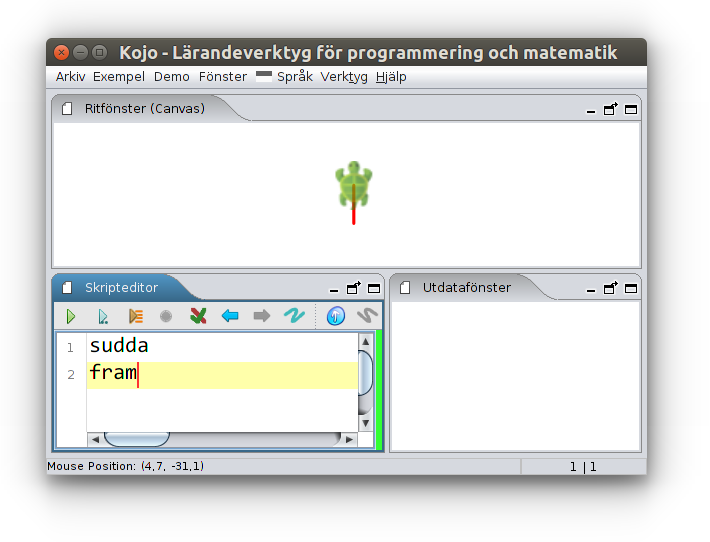
\includegraphics[width=0.8\textwidth]{../img/kojo/kojo.png}
\caption{Den nybörjarvänliga utvecklingsmiljön Kojo för Scala på svenska.}
\label{fig:appendix:ide:kojo}
\end{figure} 

\subsection{Installera Kojo}

Kojo är förinstallerat på LTH:s datorer och körs igång med kommandot \texttt{kojo}. För instruktioner om hur du installerar Kojo på din egen dator se här:\\
\href{http://www.lth.se/programmera/installera/}{lth.se/programmera/installera}

Kojo kräver att \texttt{java} finns på din dator. Eftersom du behöver tillgång till JDK i kursen, är det lika bra att installera hela JDK direkt (och inte bara JRE, så som beskrivs å länken ovan); se vidare hur du gör detta i avsnitt \ref{appendix:compile:install-jdk}. 
%\href{http://www.kogics.net/kojo-download}{www.kogics.net/kojo-download}


\subsection{Använda Kojo}

När du startar Kojo första gången, välj ''Svenska'' i språkmenyn och starta om Kojo. Därefter fungerar grafikfunktionerna på svenska enligt tabell \ref{table:kojo:functions}. När du startat om Kojo inställt på Svenska ser programmet ut ungeför som i figur \ref{fig:appendix:ide:kojo} på sidan \pageref{fig:appendix:ide:kojo}.


Det finns ett antal användbara kortkommando som du hittar i menyerna i Kojo. Undersök speciellt Ctrl+Alt+Mellanslag som ger autokomplettering baserat på det du börjat skriva.


{\small\renewcommand{\arraystretch}{1.45}
\begin{longtable}{@{}p{0.42\textwidth} p{0.55\textwidth}}

\caption{Några av sköldpaddans funktioner. Se även \href{http://lth.se/programmera}{lth.se/programmera}}\label{table:kojo:functions}\\

\emph{Svenska/Engelska} & \emph{Vad händer?}  \\ \hline
%!TEX encoding = UTF-8 Unicode
%!TEX root = ../compendium2.tex

\chapter{Kojo}\label{appendix:kojo}

\section{Vad är Kojo?}

Kojo%
\footnote{\href{https://en.wikipedia.org/wiki/Kojo_(programming_language)}{en.wikipedia.org/wiki/Kojo\_(programming\_language)}}
 är en integrerad utvecklingsmiljö för Scala som är speciellt anpassad för programmeringsundervisning i grundskolan. Kojo används i LTH:s Science Center Vattenhallen för utbildning av grundskolelärare i programmering och vid skolbesök och annan besöksverksamhet, i vilken lärare och studenter vid LTH arbetar som handledare. 
 
 Kojo är öppen källkod och utvecklingsgemenskapen leds av Lalit Pant från Indien. I Kojo finns även lättillgängliga bibliotek som gör tröskeln lägre att programmera rörlig grafik och enkla spel.

Under kursens första laboration använder vi grafikbiblioteket i Kojo för att illustrera grundläggande begrepp, så som sekvens, alternativ, repetition och abstraktion.  


\begin{figure}[H]
\centering
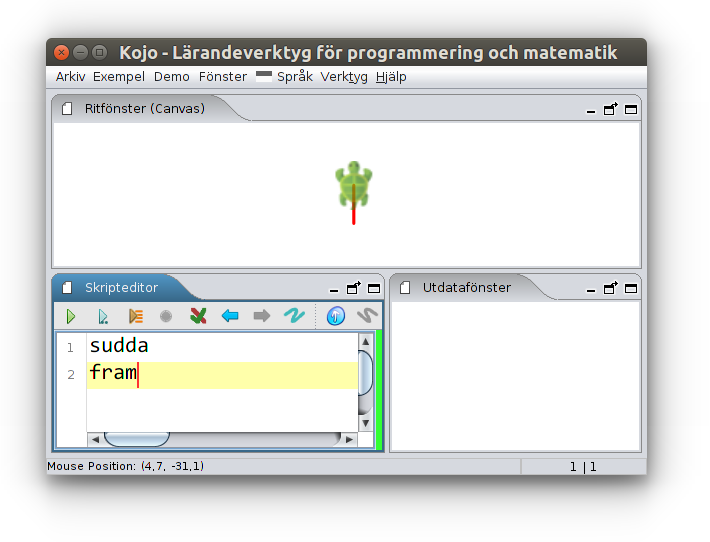
\includegraphics[width=0.8\textwidth]{../img/kojo/kojo.png}
\caption{Den nybörjarvänliga utvecklingsmiljön Kojo för Scala på svenska.}
\label{fig:appendix:ide:kojo}
\end{figure}

\section{Använda grafikbiblioteket i Kojo}\label{appendix:ide:kojo:install}

Kojo bygger på den beprövade pedagogiska idén med sköldpaddsgrafik \Eng{turtle graphics}\footnote{\url{https://en.wikipedia.org/wiki/Turtle_graphics}}, där du skriver program som styr en sköldpadda med en penna under magen. När sköldpaddan rör sig bildas ett streck av valfri färg på skärmen. Beroende på hur du bestämmer att sköldpaddan ska röra sig och vilken färg du bestämmer att pennan ska ha, kan du skapa olika intressanta bilder och samtidigt lära dig om programmeringens grunder.

Under kursens första laboration ska du använda grafikbiblioteket i Kojo tillsammans med editorn VS \code{code} och \code{scala-cli} i terminalen (se appendix \ref{appendix:terminal} och \ref{appendix:compile}). Ladda ner filen \texttt{kojo.scala} från \url{https://cs.lth.se/pgk/kojolib} och spara i en ny katalog med hjälp av din webbläsare, eller via dessa kommandon:

\begin{REPLnonum}
> mkdir w01-kojo
> cd w01-kojo
> curl -o kojolib.scala -sL https://cs.lth.se/pgk/kojolib
\end{REPLnonum}

Nu kan du starta Scala REPL och rita med Kojo så här:

\begin{REPLnonum}
> scala-cli repl .
Welcome to Scala 3.1.2 (17.0.2, Java OpenJDK 64-Bit Server VM).
Type in expressions for evaluation. Or try :help.
                                                                                                                               
scala> fram; höger; fram; vänster

\end{REPLnonum}

Du kan starta VS \code{code} i aktuellt bibliotek så här:
\begin{REPLnonum}
> code .
\end{REPLnonum}

Skriv nedan progam i VS \code{code} och spara det i samma katalog som den tidigare nedladdade filen, under ett nytt valfritt filnamn, t.ex. \code{rita.scala}:

\begin{Code}
@main def rita =
  fram; höger
  fram; vänster
\end{Code}

Kör ditt fristående program med:
\begin{REPLnonum}
> scala-cli run .
\end{REPLnonum}

Du ska nu få upp ett fönster som heter Kojo Canvas med en sköldpadda som ritat två streck. När du stänger fönstret så avslutas programmet. Prova fler sköldpaddsfunktioner enligt tabell \ref{table:kojo:functions}.

I stället för att ladda ned filen \code{kojolib.scala} så kan du placera dess innehåll på lämpligt ställe i ditt program enligt nedan. Observera att raden som börjar med \code{//> using lib} ska vara en enda lång rad utan radbrytningar. Raden med \code{export} gör Kojos kommandon tillgängliga utan prefix:
\begin{CodeSmall}[breaklines=true]
//> using scala "3"
//> using lib "net.kogics:kojo-lib:0.1.1,url=https://github.com/lunduniversity/introprog/releases/download/kojo-lib-0.1.1/kojo-lib-0.1.1.jar"

export net.kogics.kojo.Swedish.*, padda.*, CanvasAPI.*, TurtleAPI.*
\end{CodeSmall}


\noindent Scala-koden för den svenska paddans api finns här: \\
%\href{https://github.com/litan/kojo/blob/master/src/main/scala/net/kogics/kojo/lite/i18n/svInit.scala}{github.com/litan/kojo/blob/master/src/main/scala/net/kogics/kojo/lite/i18n/svInit.scala} \\
\href{https://github.com/litan/kojo-lib/blob/main/src/main/scala/net/kogics/kojo/i18n/Swedish.scala}{github.com/litan/kojo-lib/blob/main/src/main/scala/net/kogics/kojo/i18n/Swedish.scala}


%Kojo kräver (numera) \emph{inte} att \texttt{java} finns på din dator utan kommer med en egen JVM. 
%Eftersom du behöver tillgång till JDK i kursen, är det lika bra att installera hela JDK direkt (och inte bara JRE, så som beskrivs å länken ovan); se vidare hur du gör detta i avsnitt \ref{appendix:compile:install-jdk}.
%\href{http://www.kogics.net/kojo-download}{www.kogics.net/kojo-download}


{\small\renewcommand{\arraystretch}{1.4}
\begin{longtable}{@{}p{0.42\textwidth} p{0.55\textwidth}}

\caption{Ett urval av funktioner i Kojo. Se även \href{http://lth.se/programmera}{lth.se/programmera}}\label{table:kojo:functions}\\

\emph{Svenska/Engelska} & \emph{Vad händer?}  \\ \hline
\code|sudda| \newline \code|clear| & Ritfönstret suddas \\
\code|fram| \newline \code|forward()| & Paddan går framåt 25 steg. \\
\code|fram(100)| \newline \code|forward(100)| & Paddan går framåt 100 steg. \\
\code|höger| \newline \code|right(90)| & Paddan vrider sig 90 grader åt höger. \\
\code|höger(45)| \newline \code|right(45)| & Paddan vrider sig 45 grader åt höger. \\
\code|vänster| \newline \code|left(90)| & Paddan vrider sig 90 grader åt vänster. \\
\code|vänster(45)| \newline \code|left(45)| & Paddan vrider sig 45 grader åt vänster. \\
\code|hoppa| \newline \code|hop| & Paddan hoppar 25 steg utan att rita. \\
\code|hoppa(100)| \newline \code|hop(100)| & Paddan hoppar 100 steg utan att rita. \\
\code|hoppaTill(100, 200)| \newline \code|jumpTo(100, 200)| & Paddan hoppar till läget (100, 200) utan att rita. \\
\code|gåTill(100, 200)| \newline \code|moveTo(100, 200)| & Paddan vrider sig och går till läget (100, 200). \\
\code|hem| \newline \code|home| & Paddan går tillbaka till utgångsläget (0, 0). \\
\code|öster| \newline \code|setHeading(0)| & Paddan vrider sig så att nosen pekar åt höger. \\
\code|väster| \newline \code|setHeading(180)| & Paddan vrider sig så att nosen pekar åt vänster. \\
\code|norr| \newline \code|setHeading(90)| & Paddan vrider sig så att nosen pekar uppåt. \\
\code|söder| \newline \code|setHeading(-90)  | & Paddan vrider sig så att nosen pekar neråt. \\
\code|mot(100,200)| \newline \code|towards(100, 200)| & Paddan vrider sig så att nosen pekar mot läget (100, 200) \\
\code|sättVinkel(90)| \newline \code|setHeading(90)| & Paddan vrider nosen till vinkeln 90 grader. \\
\code|vinkel| \newline \code|heading| & Ger vinkelvärdet dit paddans nos pekar. \\
\code|sakta(5000)| \newline \code|setAnimationDelay(5000) | & Gör så att paddan ritar jättesakta. \\
\code|suddaUtdata| \newline \code|clearOutput| & Utdatafönstret suddas. \\
\code|utdata("hej")| \newline \code|println("hej")| & Skriver texten \texttt{hej} i utdatafönstret. \\
\code|val t = indata("Skriv")| \newline \code|val t = readln("Skriv:")| & Väntar på inmatning efter ledtexten \texttt{Skriv} och sparar den inmatade texten i t.  \\
\code|textstorlek(100)| \newline \code|setPenFontSize(100)| & Paddan skriver med jättestor text nästa gång du gör skriv. \\
\code|båge(100, 90)| \newline \code|arc(100, 90)| & Paddan ritar en båge med radie 100 och vinkel 90. \\
\code|cirkel(100)| \newline \code|circle(radie)| & Paddan ritar en cirkel med radie 100. \\
\code|synlig| \newline \code|visible| & Paddan blir synlig. \\
\code|osynlig| \newline \code|invisible| & Paddan blir osynlig. \\
\code|läge.x| \newline \code|position.x| & Ger paddans x-läge \\
\code|läge.y| \newline \code|position.y| & Ger paddans y-läge \\
\code|pennaNer| \newline \code|penDown| & Sätter ner paddans penna så att den ritar när den går. \\
\code|pennaUpp| \newline \code|penUp| & Lyfter upp paddans penna så att den INTE ritar när den går. \\
\code|pennanÄrNere| \newline \code|penIsDown| & Kollar om pennan är nere eller inte. \\
\code|färg(rosa)| \newline \code|setPenColor(pink)| & Sätter pennans färg till rosa. \\
\code|fyll(lila)| \newline \code|setFillColor(purple)| & Sätter ifyllnadsfärgen till lila. \\
\code|fyll(genomskinlig)| \newline \code|setFillColor(noColor)| & Gör så att paddan inte fyller i något när den ritar. \\
\code|bredd(20)| \newline \code|setPenThickness(20)| & Gör så att pennan får bredden 20. \\
\code|sparaStil| \newline \code|saveStyle| & Sparar pennans färg, bredd och fyllfärg. \\
\code|laddaStil| \newline \code|restoreStyle| & Laddar tidigare sparad färg, bredd och fyllfärg. \\
\code|sparaLägeRiktning| \newline \code|savePosHe| & Sparar pennans läge och riktning \\
\code|laddaLägeRiktning| \newline \code|restorePosHe| & Laddar tidigare sparad riktning och läge \\
\code|siktePå| \newline \code|beamsOn| & Sätter på siktet. \\
\code|sikteAv| \newline \code|beamsOff| & Stänger av siktet. \\
\code|bakgrund(svart)| \newline \code|setBackground(black)| & Bakgrundsfärgen blir svart. \\
\code|bakgrund2(grön,gul)| \newline \code|setBackgroundV(green, yellow)| & Bakgrund med övergång från grönt till gult. \\
\code|upprepa(4){fram; höger}| \newline \code|repeat(4){forward; right}| & Paddan går fram och svänger höger 4 gånger. \\
\code|avrunda(3.99)| & Avrundar 3.99 till 4.0 \\
\code|slumptal(100)| & Ger ett slumptal mellan 0 och 99. \\
\code|slumptalMedDecimaler(100)| & Ger ett slumptal mellan 0 och 99.99999999 \\
\code|systemtid| & Ger nuvarande systemklocka i sekunder. \\
\code|räknaTill(5000)| & Kollar hur lång tid det tar för din dator att räkna till 5000. \\


\end{longtable}
}%end small


\section{Kojo Desktop}

Kojo finns som fristående skrivbordsapplikation, kallad Kojo Desktop. Kojo Desktop innehåller en egen editor med syntaxfärgning för Scala, men fungerar ännu så länge bara för Scala 2. En av de synligaste skillnaderna mellan Scala 2 och Scala 3 är att klammerparenteser vid flerradiga funktioner är nödvändiga i Scala 2, medan Scala 3 har valfria klammerparenteser. Så om du använder Kojo Desktop behöver du komma ihåg att omgärda sekvenser av rader som hör ihop med \code|{| och \code|}|. 

Kojo Desktop är förinstallerat på LTH:s datorer och körs igång med terminalkommandot \texttt{kojo} eller via applikationsmenyn.  För instruktioner om hur du installerar Kojo Desktop på din egen dator se här: \href{http://www.lth.se/programmera/installera/}{lth.se/programmera/installera}

När du startar Kojo första gången, välj ''Svenska'' i språkmenyn och starta om Kojo. Därefter fungerar grafikfunktionerna på svenska enligt tabell \ref{table:kojo:functions}. När du startat om Kojo inställt på svenska ser programmet ut ungefär som i figur \ref{fig:appendix:ide:kojo} på sidan \pageref{fig:appendix:ide:kojo}.

Det finns ett antal användbara kortkommando som du hittar i menyerna i Kojo Desktop. Undersök speciellt Ctrl+Alt+Mellanslag som ger autokomplettering baserat på det du börjat skriva.

\section{Kojo i Webbläsaren}

En begränsad variant av Kojo finns tillgänglig för programmering direkt i din webbläsare här: \url{http://kojo.lu.se/}

När du trycker på play-knappen så kompileras din kod på en server till Javascript via ScalaJS och därefter körs Javascript-koden i din webbläsare. 
Kojo på webben är också ännu så länge begränsad till Scala 2 och kräver att du omgärdar sekvenser av rader som hör ihop med \code|{| och \code|}|.


\section{Mer om Kojo}

I detta dokument finns en enkel introduktion till Kojo: \\ ''Introduction to Kojo'' \url{http://www.kogics.net/kojo-ebooks#intro}


\hline
\end{longtable}
}%end small

\noindent Scala-koden för den svenska paddans api finns här: \\
\href{https://bitbucket.org/lalit_pant/kojo/src/tip/src/main/scala/net/kogics/kojo/lite/i18n/svInit.scala}{bitbucket.org/lalit\_pant/kojo/src/tip/src/main/scala/net/kogics/\\kojo/lite/i18n/svInit.scala}




\newpage

\section{Eclipse och ScalaIDE}\label{appendix:ide:eclipse}

Eclipse%
\footnote{\href{https://en.wikipedia.org/wiki/Eclipse_(software)}{en.wikipedia.org/wiki/Eclipse\_(software)}}
är en professionell IDE som stödjer många olika programmeringsspråk. Eclipse är skriven i Java och bygger vidare på ett utvecklingsprojekt som initierades av IBM. Eclipse är ett fritt och öppet projekt som numera kontrolleras av en oberoende stiftelse.

Till Eclipse finns en insticksmodul \Eng{plug-in} som kallas ScalaIDE och erbjuder stöd för Scala med tillhörande standardbibliotek.

Eclipse är en omfattande och avancerad programmeringsmiljö med många funktioner och inställningar. Det finns även en omfattande uppsättning insticksmoduler och tilläggsprogram som underlättar utveckling av t.ex. webbprogram, databaser och mycket annat. 

I detta avsnitt ges länkar till installation samt tips om hur du kommer igång med att använda Eclipse och ScalaIDE. Det går ganska snabbt att lära sig grunderna, men det kräven en viss ansträngning att lära sig de mer avancerade funktionerna. Det finns omfattande resurser på nätet som hjälper dig vidare. 


\subsection{Installera Eclipse Mars och ScalaIDE}\label{appendix:ide:eclipse:install}

Eclipse med ScalaIDE är förinstallerat på LTH:s datorer och startas med kommandot \texttt{scalaide} i ett terminalfönster.

ScalaIDE fungerar med Eclipse-versionerna \textit{Luna} och \textit{Mars} (men i skrivande stund fungerar ScalaIDE ännu \textit{inte} med den allra senaste versionen kallad \textit{Neon}). 

För att installera ScalaIDE på din egen dator, följ nedan instruktioner: 

\begin{enumerate}
\item Kontrollera enligt avsnitt \ref{appendix:compile:check-jdk} att du har \texttt{java} installerat och installera vid behov JDK enligt avsnitt \ref{appendix:compile:install-jdk}.

\item Installera Eclipse version \textbf{Mars}, varianten för \textbf{Java Developers} som återfinns på denna sida: \\ \url{https://www.eclipse.org/downloads/packages/release/Mars/2} \\ som är den \textit{andra} varianten i listan (alltså inte Java EE). Följ dessa steg:
\begin{enumerate}
\item Klicka på den \textbf{64-bit}-variant som passar ditt operativsystem.
\item Filen som laddas ner heter något som liknar (beroende på OS): \\ \texttt{eclipse-java-mars-2-win32-x86\_64.zip} 
\\ Det kan ta lång tid att ladda ner filen som är på ca 170MB. Om du klickar på \textit{''select a mirror''} kan du välja en svensk sajt för att ladda ner snabbare. 

\item Dubbelklicka på filen för att packa upp den, vilket kan ta många minuter. Du får, när upppackningen är klar, ett bibliotek med en fungerande Eclipse-installation som du kan placera var du vill. Kör du Windows, lägg den förslagsvis här:\\ 
\code|C:\eclipse\eclipse-java-mars-2-win32-x86_64|

\item för Ubuntu Linux finns kompletterande installationsanvisningar här, som ger dig en ikon i app-menyn m.m.: 
\\ \url{http://askubuntu.com/questions/26632/how-to-install-eclipse}
\end{enumerate}

\item Installera Scala IDE inifrån%
\footnote{Det finns på ScalaIDE-hemsidan möjlighet att ladda ner en Eclipse-variant med färdiginstallerad ScalaIDE-plugin, men då får du i skrivande stund den gamla versionen Eclipse \textit{Luna}, varför du rekommenderas att, enligt instruktionerna här, själv installera ScalaIDE inifrån Eclipse \textit{Mars}, som är den senaste Eclipse-versionen för vilken ScalaIDE fungerar.}
 Eclipse enligt nedan steg:
\begin{enumerate}
\item Starta Eclipse, t.ex. genom att köra igång den exekverbara filen som ligger i underbiblioteket \texttt{eclipse}, i Windows heter den \texttt{eclipse.exe} medan den exekverbara filen i Linux heter \texttt{eclipse} utan filändelse.

\item Välj i frågerutan som dyker upp, någon plats för \textit{workspace} (kvittar vilken just nu, kan ändras senare).

\item Klicka på menyn \textit{Help} $\rightarrow$ \textit{Install new software}.

\item Klicka på \textit{Add}-knappen till höger och skriv: \\ \textit{''ScalaIDE for Scala 2.11''} i \textit{Name}-fältet och ange denna adress i \textit{Location}-fältet: \\
  {\small\mbox{\url{http://download.scala-ide.org/sdk/lithium/e44/scala211/stable/site}}} \\
  och klicka \textit{OK}.
  
\item Du får nu upp en lista med alternativ. Kryssa för alternativet
\\ {\frame{\checkmark}}~~\textit{Scala IDE for Eclipse} \\ och klicka \textit{Next} och sedan \textit{Next} igen och acceptera licensvillkoren och klicka \textit{Finish}.

\item Låt installationen ta sin tid och starta sedan om Eclipse när installationen är färdig. 

\item När Eclipse är igång igen visas en dialog som föreslår att du ska köra \textit{Setup Diagnostics}. Gör detta och välj \textit{Use recommended default settings}. Ändra även i filen \textbf{eclipse.ini} för höja den övre minnesgränsen. Det gör du genom att ändra på den rad i filen som börjar med \texttt{-Xmx}. Hur mycket du ska tillåta som max beror på hur mycket minne du har, men ge minst 1 gigabyte för smidig körning, genom att skriva så här på relevant rad i filen \textbf{eclipse.ini}: \\
\texttt{-Xmx1G } \\


\item Kompletterande information finns här, inklusive en video som visar installationsproceduren och hur man kommer igång med ett ''hello world''-program: \\ \url{http://scala-ide.org/download/current.html}


\end{enumerate}


\end{enumerate}

\noindent I nästa avsnitt beskrivs några rekommenderade anpassningar som du kan göra bland de omfattande inställningsmöjligheterna för Eclipse.

\newpage

\subsection{Anpassa Eclipse och ScalaIDE}\label{subsection:appendix:ide:eclipse:tweaks}

\newcommand\Menu[1]{\textit{#1}}
\newcommand\MenuArrow[1]{\Menu{#1}~$\rightarrow$~}
\newcommand\FramedCheckmark[1]{~\frame{\checkmark}~~\textbf{#1}}
\newcommand\FramedUnchecked[1]{$\Box$~\textbf{#1}}
\newcommand\Button[1]{\fbox{\textbf{#1}}}
\newcommand\EclipsePrefs{\MenuArrow{Window}\MenuArrow{Preferences}}
\newcommand\EclipsePrefsGeneral{\EclipsePrefs\MenuArrow{General}}


Förutom maxminneshöjningen i filen \texttt{eclipse.ini}, som finns i installationskatalogen för Eclipse, till minst \texttt{-Xmx1G } (se föregående avsnitt), är det bra att göra några ytterligare anpassningar av Eclipse och ScalaIDE för att få en snabbare och smidigare utvecklingsmiljö. Du hittar inställningarna i menyn \EclipsePrefs ... uppe till höger i Eclipse-fönstret.



\begin{enumerate}
\item \EclipsePrefsGeneral 
\\ Markera \FramedCheckmark{Show Heap Status} så får du se minnesanvändningen i en liten ruta i nederdelen av fönstret, vilket hjälper dig att upptäcka om minnesbegränsningen i filen \texttt{eclipse.ini} är en flaskhals vid stora projekt och många öppna fönster. Klicka sedan \Button{Apply} längst ner.

\item \label{item:scala-perspective} \EclipsePrefsGeneral\MenuArrow{Editors}\MenuArrow{Perspective}  
\\ Markera \textit{Scala} i listan med perspektiv och klicka på knappen 
 \\ \Button{Make default} till höger och sedan på knappen \Button{Apply} längst ner.

\item \EclipsePrefsGeneral\MenuArrow{Editors}\MenuArrow{TextEditors}
\\ Markera \FramedCheckmark{Insert spaces for tabs} så att du slipper specialtecken som kan tolkas olika av olika editorer. Klicka sedan \Button{Apply} längst ner.

\item \EclipsePrefsGeneral\MenuArrow{Editors}\MenuArrow{TextEditors}
\\ \MenuArrow{Spelling} Avmarkera \FramedUnchecked{Enable spell checking} för att slippa att svenska namn och svenska kommentarer markeras som felstavade. Om du senare jobbar med ett projekt helt på engelska, kan du med fördel markera denna kryssruta igen. Klicka sedan \Button{Apply} längst ner.

\item \EclipsePrefsGeneral\MenuArrow{Editors}\MenuArrow{Webbrowser}
\\ Markera \FramedCheckmark{Use external web browser} för att köra din vanliga webbläsare när du klickar på länkar. Klicka sedan \Button{Apply} längst ner.
  
\item  \EclipsePrefs\MenuArrow{Scala}\MenuArrow{Compile}
\\ I fliken \textbf{Standard} markera dessa kryssrutor för att få extra varningar: \\
\begin{tabular}{l @{}l @{}l}
\textit{deprecation} & \FramedCheckmark{} & varnar vid användning av föråldrad kod som snart utgår \\
\textit{feature}     & \FramedCheckmark{} & påminner om import vid användning av avancerad kod  \\
\textit{unchecked}   & \FramedCheckmark{} & ger tips vid speciella problem med generiska typer \\
\end{tabular}\\
och klicka sedan på knappen \Button{Apply} längst ner.

\item \EclipsePrefs\MenuArrow{Java}\MenuArrow{Compiler}\MenuArrow{Errors/Warnings}
\\ Veckla ut listan \textbf{Potential programming problems} och sätt \textbf{Resource leak} till alternativet \textbf{Ignore}, så slipper du varningar vid användning \jcode{Scanner} i Java. Klicka sedan \Button{Apply} längst ner.

\end{enumerate}

\noindent Ovan anpassningar är rekommenderade men inte nödvändiga och du kan gärna välja att göra andra anpassningar som passar just dig. Skriv då gärna ner vilken inställning du ändrat, så att du hittar tillbaka om du ångrar dig. 

Du hittar tips om fler inställningar för att anpassa ScalaIDE här: \\
\url{http://scala-ide.org/docs/current-user-doc/advancedsetup}



\subsection{Använda Eclipse och ScalaIDE}\label{appendix:ide:eclipse:use}

Ett grundläggande koncept i Eclipse är \textbf{workspace}. Ett workspace utgör ett arbetsområde kopplat till en katalog i ditt filsystem där du kan arbeta med ett eller flera \textbf{projekt}. Ett projekt innehåller i sin tur dina källkodsfiler och klassfiler etc. i en specifik katalogstruktur som Eclipse skapar när du editerar, kompilerar och kör dina projekt. 

\subsubsection{Starta och välja workspace}\label{subsubsection:start:eclipse}

När du startar Eclipse måste du välja vilket workspace du vill använda innan du kommer vidare. När du kör igång Eclipse första gången, klicka OK enligt det förslag som ges. Du kan senare växla workspace genom menyn \MenuArrow{File}\Menu{Switch Workspace}. Om katalogen du anger inte redan finns, kommer den att skapas och initieras med de filer Eclipse behöver.

I figur \ref{fig:appendix:eclipse:welcome} visas välkomstfliken i Eclipse med sina länkar till funktionsöversikt och olika handledningar. Stäng välkomstfliken genom att klicka på flikens kryss eller på ikonen \textit{Workbench}. Då kommer du vidare till den normala arbetsytan i Eclipse. Du kan få tillbaka välkomstfliken igen via menyn \MenuArrow{Help}\Menu{Welcome}. 

\begin{figure}[H]
\centering
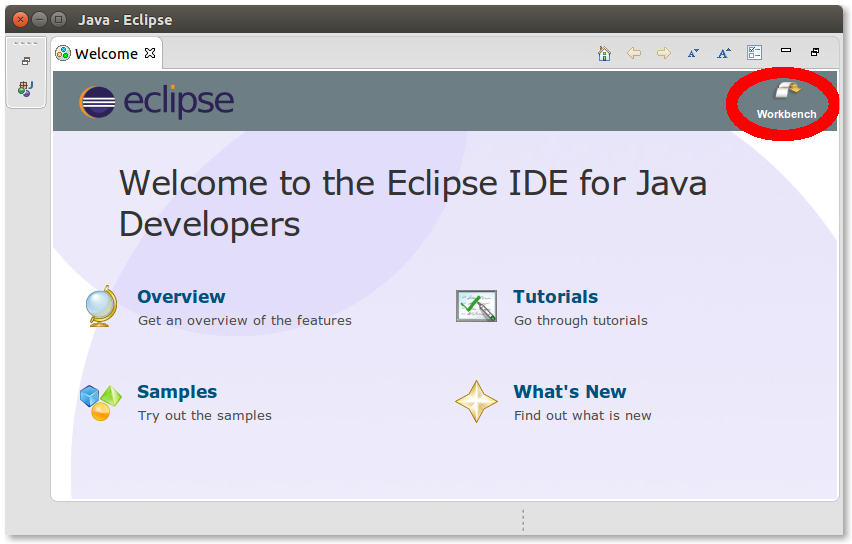
\includegraphics[width=1.0\textwidth]{../img/eclipse/eclipse-welcome.png}
\caption{Välkomstfliken för Eclipse, som nås via menyn \MenuArrow{Help}\Menu{Welcome}. Gå vidare genom att klicka på \textit{Workbench}.}
\label{fig:appendix:eclipse:welcome}
\end{figure}

\subsubsection{Välja perspektiv och visa olika vyer}

Eclipse-fönstret kan innehålla många underfönster i olika flikar, så kallade \textbf{views} eller vyer, som kan arrangeras på olika vis efter hur du vill ha dem. Vilka vyer som syns och hur de placeras beror på vilket s.k. \textbf{perspective} som är aktivt.  Figur \ref{fig:appendix:eclipse:open-perspective} visar arbetsytan med olika vyer i Java-perspektivet. 

Du kan byta till Scala-perspektivet genom att trycka på 
\includegraphics[scale=0.75]{../img/eclipse/eclipse-perspective-button.png} eller genom menyn \MenuArrow{Window}\MenuArrow{Perspective}\MenuArrow{Open Perspective}\MenuArrow{Other...}\Menu{Scala}.
Du kan anpassa inställningarna så att Scala blir \textit{default perspective}, se steg \ref{item:scala-perspective} i avsnitt \ref{subsection:appendix:ide:eclipse:tweaks} på sidan \pageref{subsection:appendix:ide:eclipse:tweaks}.

Stäng vyerna \textit{Task List} och \textit{Outline} om du vill ha mer plats till de övriga vyerna för paketnavigering, editering och utdata. Du kan öppna stängda vyer igen genom menyn \MenuArrow{Window}\Menu{Show View}. 

\begin{figure}
\centering
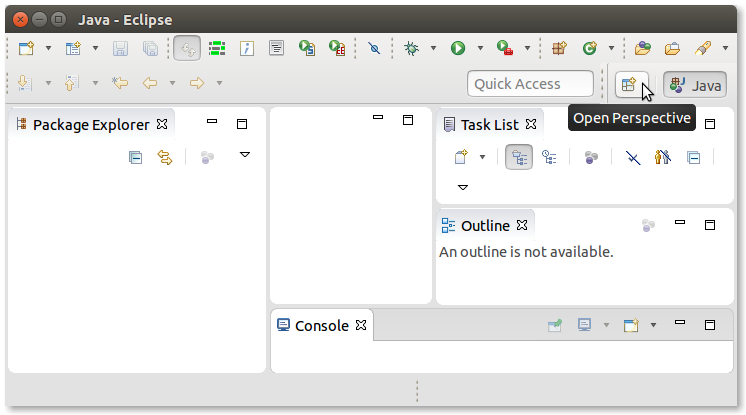
\includegraphics[width=1.0\textwidth]{../img/eclipse/eclipse-open-perspective.png}
\caption{Arbetsytan i Eclipse. Du kan växla mellan Scala- och Java-perspektivet genom att klicka på perspektivvalsknappen.}
\label{fig:appendix:eclipse:open-perspective}
\end{figure}

\subsubsection{Hello World}\label{subsubsection:eclipse:hello-world}

Efter att du öppnat Eclipse med ScalaIDE i ett tomt workspace och valt Scala-perspektivet enligt föregående avsnitt, kan du skapa ditt första projekt med ett \textit{''Hello World''}-program enligt stegen nedan.

\begin{enumerate}
\item Högerklicka i \Menu{Package Explorer} och välj \MenuArrow{New}\Menu{Scala Project}, varefter en dialogruta visas. 

\item Fyll i namnet \texttt{hello} i fältet \Menu{Project Name} och klicka \Button{Finish}.

\item Högerklicka igen i \Menu{Package Explorer} och välj \MenuArrow{New}\Menu{Scala Object}, varefter en ny dialogruta visas. 

\item Fyll i namnet \texttt{hi} i fältet \Menu{Project Name} och klicka \Button{Finish}.

\item Du får nu i editorvyn ett kodskellet med \code{object hi}.

\item Börja skriv \code{main} som visas i figur \ref{fig:appendix:eclipse:complete-main} och tryck Ctrl+Mellanslag för att aktivera kodkomplettering \Eng{code completion}. Då får du upp en lista med alternativ. Välj det översta alternativet \texttt{main} varefter ett kodskellet med en main-metod klistras in automatiskt i din kod.

\begin{figure}
\centering
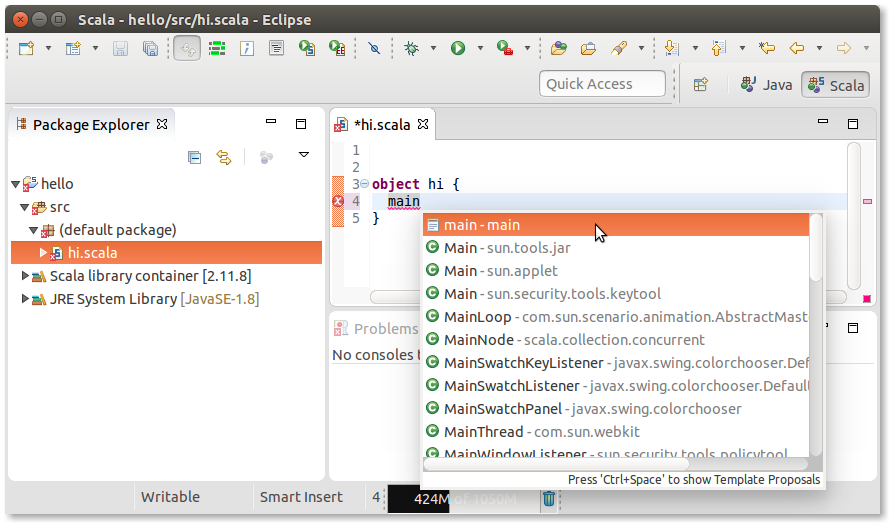
\includegraphics[width=1.0\textwidth]{../img/eclipse/eclipse-complete-main.png}
\caption{Aktivera kodkomplettering med Ctrl+Mellanslag efter ordet \code{main}.}
\label{fig:appendix:eclipse:complete-main}
\end{figure}

\item Fyll i lämplig utskriftstext i ett \code{println}-anrop så att din \code{main}-metod blir så som visas i editorfliken i figur \ref{fig:appendix:eclipse:hello-world}.

\begin{figure}[H]
\centering
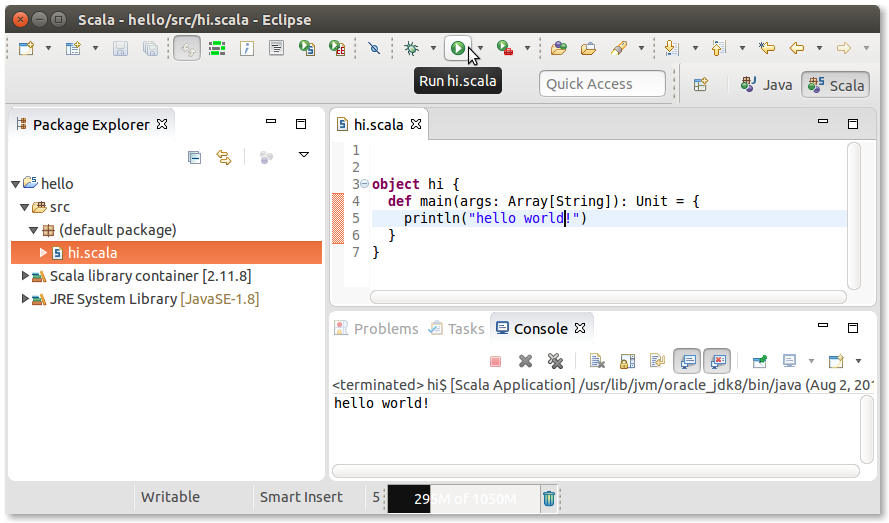
\includegraphics[width=1.0\textwidth]{../img/eclipse/eclipse-hello-world.png}
\caption{Skriv klart \code{main}-metoden och kör ditt program med play-knappen.}
\label{fig:appendix:eclipse:hello-world}
\end{figure}

\item Kör ditt program genom att trycka på den gröna play-knappen, som muspekaren i figur \ref{fig:appendix:eclipse:hello-world} pekar på. Du kan också trycka F11 för att köra igång din app, efter att du vid första körningen i dialogen \textit{Select Preferred Launcher} markerat  \FramedCheckmark{Use configuration specific settings} och valt alternativet \textit{Scala Application (new debugger) Launcher}. 

\end{enumerate}




\subsubsection{Ladda ner kursens workspace och importera projekt till labbarna}

Det finns en zip-fil med ett workspace med projekt för flera av kursens laborationer som du kan ladda ner och importera i Eclipse. Följ stegen nedan.

\begin{enumerate}
\item Ladda ner kursens workspace här: \url{http://cs.lth.se/pgk/ws}

\item Packa upp filen på lämpligt ställe.

\item Starta Eclipse med ScalaIDE-plugin (se startinstruktioner på sidan \pageref{subsubsection:start:eclipse}). 

\item Växla workspace till biblioteket du nyss packade upp, ungefär som i figur \ref{fig:eclipse:ide:open} och klicka \Button{OK}.
\begin{figure}[H]
\centering
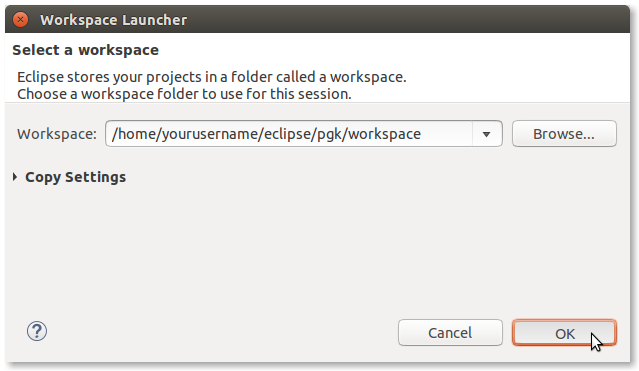
\includegraphics[width=1.0\textwidth]{../img/eclipse/eclipse-select-workspace.png}
\caption {Öppna kursens workspace genom att bläddra till biblioteket där du packade upp filen som du laddat ned från: \url{http://cs.lth.se/pgk/ws} }
\label{fig:eclipse:ide:open}
\end{figure}

\item Stäng välkomstfliken för att komma vidare till workbench (se figur \ref{fig:appendix:eclipse:welcome} på sidan \pageref{fig:appendix:eclipse:welcome}). Det ser då ut ungefär som i figur~\ref{fig:appendix:eclipse:open-perspective} på sidan \pageref{fig:appendix:eclipse:open-perspective}. Det syns ännu inget i \textit{Package Explorer} då vi ännu inte importerat något projekt. 

\item Innan du går vidare, säkerställ att du har Scala-perspektivet aktiverast. Du kan växla till Scala-perspektivet genom att trycka på 
\includegraphics[scale=0.75]{../img/eclipse/eclipse-perspective-button.png} eller genom menyn \MenuArrow{Window}\MenuArrow{Perspective}\MenuArrow{Open Perspective}\MenuArrow{Other...}\Menu{Scala}.
Du kan anpassa inställningarna så att Scala blir \textit{default perspective}, se steg \ref{item:scala-perspective} i avsnitt \ref{subsection:appendix:ide:eclipse:tweaks} på sidan \pageref{subsection:appendix:ide:eclipse:tweaks}.


\item Högerklicka i \textit{Package Explorer} och välj \Menu{Import...}, se Fig.~\ref{fig:eclipse:import}, eller välj menyn \MenuArrow{File}\Menu{Import...}. 

\begin{figure}[H]
\centering
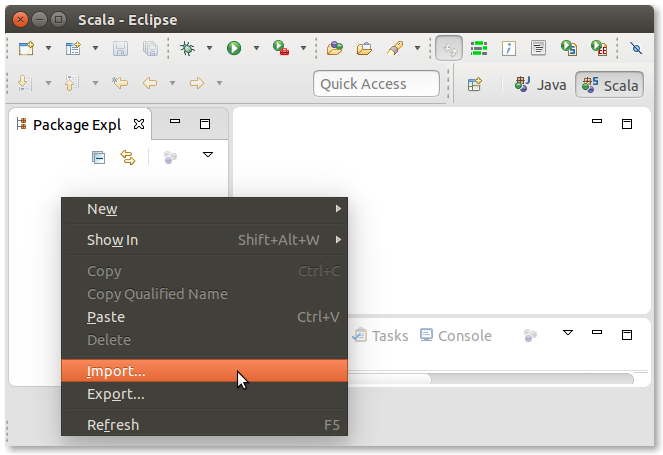
\includegraphics[width=1.0\textwidth]{../img/eclipse/eclipse-import.png} 

\caption {Välj \Menu{Import}-menyn för att importera existerande projekt.}
\label{fig:eclipse:import}
\end{figure}

\item Nu öppnas \Menu{Import}-dialogen som visas i figur \ref{fig:eclipse:import-existing}. Öppna mappen \Menu{General}, markera \textbf{Existing Projects into Workspace} och klicka \Button{Next}.



\begin{figure}[H]
\centering
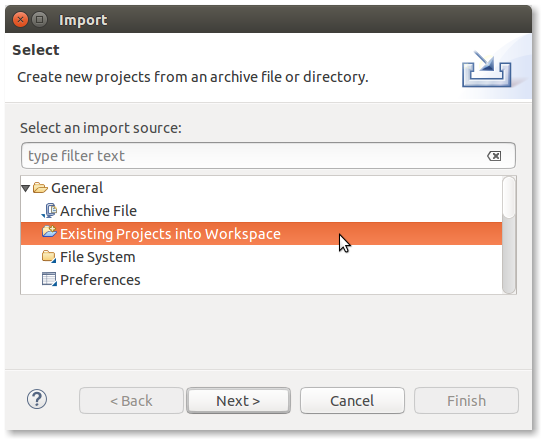
\includegraphics[width=0.75\textwidth]{../img/eclipse/eclipse-import-existing.png} 

\caption {Välj att importera existerande projekt under \Menu{General}.}
\label{fig:eclipse:import-existing}
\end{figure}


\begin{figure}[H]
\centering
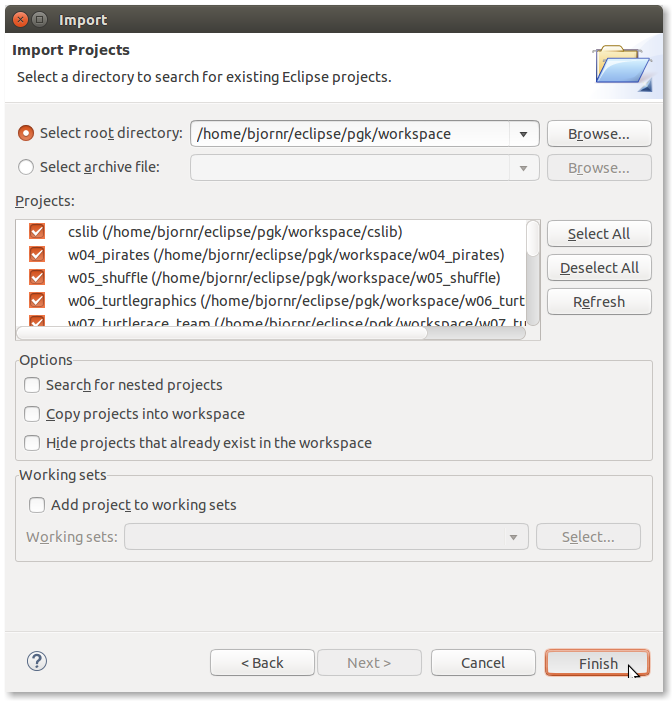
\includegraphics[width=1.0\textwidth]{../img/eclipse/eclipse-import-projects.png} 

\caption {Välj \FramedCheckmark{Select Root Directory} och klicka \Button{Browse}.}
\label{fig:eclipse:import-projects}
\end{figure}


\item Nu kommer ytterligare ett dialogfönster som visas i figure \ref{fig:eclipse:import-projects}. Med \FramedCheckmark{Select Root Directory} markerad kan du klicka \Button{Browse} för att ange workspace-mappen i ännu en dialog där du bara ska trycka \Button{Ok} utan att välja underbibliotek till workspace. När det är klart ska det se ut som i figur \ref{fig:eclipse:import-projects} där alla Eclipse-projekt \FramedCheckmark{cslib}, \FramedCheckmark{w04\_pirates}, etc. är markerade. Klicka sedan \Button{Finish}.

\item Följ ''Hello World''-instruktionerna på sidan \pageref{subsubsection:eclipse:hello-world} och skapa programmet som visas i figure \ref{fig:eclipse:pirates-hi}, genom att veckla ut projektet \textbf{w04\_pirates}, markera och högerklicka på paketet \textbf{priates}, och välja \MenuArrow{New}\Menu{Scala Object}.

\begin{figure}[H]
\centering
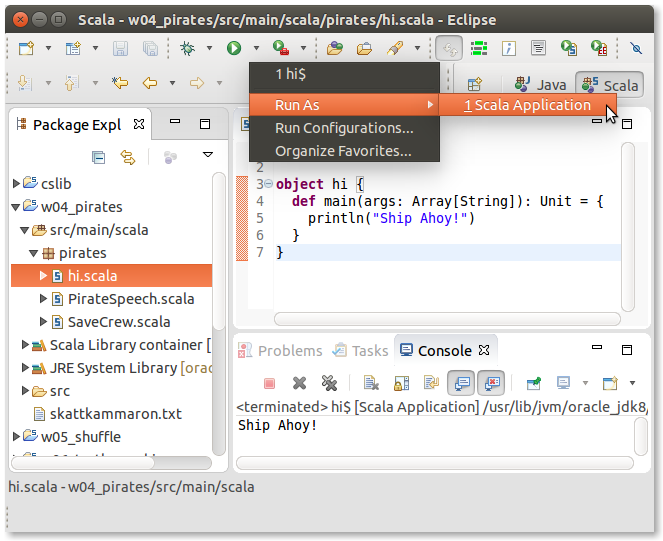
\includegraphics[width=1.0\textwidth]{../img/eclipse/eclipse-pirates-hi.png} 

\caption {Skapa ett \MenuArrow{New}\Menu{Scala Object} med kod enligt bilden.}
\label{fig:eclipse:pirates-hi}
\end{figure}


\end{enumerate}



\newpage

\section{IntelliJ IDEA}\label{appendix:ide:intellij}

IntelliJ IDEA%
\footnote{\href{https://en.wikipedia.org/wiki/IntelliJ_IDEA}{en.wikipedia.org/wiki/IntelliJ\_IDEA}}
 är en professionell IDE som stödjer många olika programmeringsspråk. IntelliJ är skriven i Java och utvecklas av det tjeckiska företaget JetBrains. 

IntelliJ IDEA finns i två varianter: en gratis gemenskapsvariant med öppenkällkodslicens \Eng{Community edition}, samt en betalvariant med stängd källkod och support-tjänster.


Till IntelliJ IDEA finns en insticksmodul \Eng{plug-in} som erbjuder stöd för Scala med tillhörande standardbibliotek..

IntelliJ IDEA är en omfattande och avancerad programmeringsmiljö med många funktioner och inställningar. Det finns även en omfattande uppsättning insticksmoduler och tilläggsprogram som underlättar utveckling av t.ex. webbprogram, databaser och mycket annat. 

I detta avsnitt ges länkar till installation samt tips om hur du kommer igång med att använda IntelliJ IDEA med Scala. Det går ganska snabbt att lära sig grunderna, men det kräven en viss ansträngning att lära sig de mer avancerade funktionerna. Det finns omfattande resurser på nätet som hjälper dig vidare. 

Google tillkännagav 2013 att företaget övergår från Eclipse till IntelliJ som den officiellt understödda utvecklingsmiljön för Android och 2014 lanserades utvecklingsmiljön AndroidStudio%
\footnote {\href{https://en.wikipedia.org/wiki/Android_Studio}{en.wikipedia.org/wiki/Android\_Studio}}
 som bygger vidare på IntelliJ. 

\subsection{Installera IntelliJ med Scala}\label{appendix:ide:intellij:install}

IntelliJ med Scala-plug-in är förinstallerat på LTH:s datorer och startas med kommandot \texttt{intellij} i ett terminalfönster.

\TODO Beskriv hur man installerar IntelliJ med Scala

\subsection{Använda IntelliJ}\label{appendix:ide:intellij:use}

\TODO 

%!TEX encoding = UTF-8 Unicode
%!TEX root = ../compendium1.tex

\chapter{Fixa buggar}\label{appendix:debug}

\begin{figure}[H]
\centering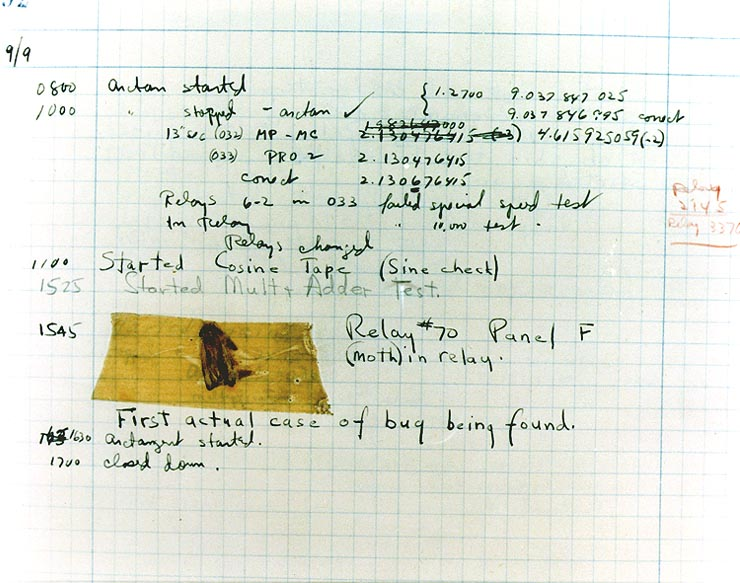
\includegraphics[width=0.85\textwidth]{../img/bug}

\caption{Den första dokumenterade buggen hittades 9 september 1947 i en Mark II Aiken Relay Calculator av Grace Hopper.\protect\footnotemark}

\end{figure}\footnotetext{\href{https://commons.wikimedia.org/w/index.php?curid=165211}{commons.wikimedia.org/w/index.php?curid=165211} Courtesy of the Naval Surface Warfare Center, Dahlgren, VA., 1988. - U.S. Naval Historical Center Online Library Photograph NH 96566-KN, Public Domain.   }


\section{Vad är en bugg?}

En bugg, även kallad lus \Eng{bug}, är en felaktighet som kan göra så att ett program inte beter sig som det är tänkt, och kan innebära oönskad utdata, att programmet kraschar, eller till och med ond bråd död.\footnote{\href{https://www.theguardian.com/technology/2016/jul/01/tesla-driver-killed-autopilot-self-driving-car-harry-potter}{www.theguardian.com/technology/2016/jul/01/tesla-driver-killed-autopilot-self-driving-car-harry-potter}}

Ursprunget till ordets användning i programmeringssammanhang är något oklar, men kan härledas till engelskans \emph{bug} som betyder insekt eller småkryp. 
Man brukar berätta att vid en felsökning av ett program som körde i en tidig dator byggd med  elektromekaniska reläer, uppdagades en död nattfjäril ihjälklämd mellan drivankaret och spolen i ett relä, som orsakade att programmet inte kunde exekveras korrekt. 



\subsection{Olika sorters fel}

När man ska lära sig mer om fel i programvarubaserade system, och hur de kan åtgärdas, är det viktigt att noga skilja på \textbf{misstag} \Eng{mistake}, \textbf{felorsak} \Eng{fault} och \textbf{felyttring} \Eng{failure}. 
Med ''misstag'' menar vi här ett fel som begås av människor (utvecklare, systemadministratörer, operatörer, användare, etc.) medan de skapar och använder ett programvarusystem. 

Det kan bli fel i olika delar av processen: 
\begin{itemize}
\item \textbf{Kravfel} uppstår medan man tänker ut vad systemet ska göra och då misstar sig angående  användarnas behov och önskemål.
\item \textbf{Designfel} uppkommer när man utformar systemets struktur på ett dåligt sätt.
\item \textbf{Implementeringsfel} begås när man programmerar och skriver felaktiga kodrader. 
\item \textbf{Testfel} förekommer vid provkörning av systemet då testkoden är felaktig och därför ger falskt alarm om ''fel'', trots att beteendet egentligen är korrekt.  
\item \textbf{Operatörsfel} sker när systemet lämnas över till de, som ska installera och köra systemet i skarp produktion, och där systemdriften \Eng{operations, ''ops''} sköts på ett sätt som får problematiska konsekvenser.
\item \textbf{Användarfel} händer då användarna ger felaktig indata, eventuellt i strid med riktlinjerna för hur systemet ska användas, som systemet inte klarar att hantera korrekt, varpå mer eller mindre allvarliga felbeteenden hos systemet följer.
\end{itemize} 
I olika delar av utvecklingsprocessen kan alltså misstag begås som, antingen omedelbart, eller någon gång i framtiden, kan orsaka fel. Men det är inte säkert att ett fel någonsin kommer att märkas. Kanske kommer de felaktiga kodraderna, som \emph{skulle} kunna orsaka ett fel, aldrig att exekveras. Eller så kommer ingen användare att någonsin vilja använda systemet så som stipuleras av (onödiga) krav. Det är alltså först när fel \emph{yttrar} sig vid exekvering som misstag märks.

Fel kan också kategoriseras utifrån \emph{hur} de upptäcks i utvecklingsprocessen. Man brukar skilja på fel upptäckta vid granskning, kompileringsfel och exekveringsfel, som diskuteras nedan:
\begin{itemize}
\item Fel upptäckta vid \textbf{granskning}. Ett effektivt sätt att upptäcka fel är att människor noga läser igenom sin egen, och andras kod och försöker leta efter möjliga problem och brister. Man blir ofta ''hemmablind'' när det gäller ens egen kod. Därför kan någon annans, oberoende granskning med ''nya, friska'' ögon vara mycket fruktbar.  I samband med kodgranskning kan man med fördel försöka bedöma  huruvida koden är lätt att läsa, lätt att ändra i eller om koden har andra viktiga kvaliteter som har betydelse för den framtida utvecklingen av koden. Ofta hittar man vid granskning även enkla programmeringsmisstag, så som felaktiga villkor och loop-räknare som inte räknas upp på rätt sätt etc.
  
\item \textbf{Kompileringsfel} uppkommer under kompilering och upptäcks tack vare kontroller som sker av  kompilatorn. 

Vid kompileringsfel får man också ofta av kompilatorn reda på \emph{var} i koden det är fel och \emph{varför} det är fel, så att sökandet efter felorsaken och åtgärdandet av misstaget underlättas. Men ibland är felmeddelandet från kompilatorn missvisande och pekar på helt fel ställe i koden, så det gäller att inte alltid lita blint på det kompilatorn skriver. Dessutom är felmeddelanden från kompilatorn ofta uttryckta i termer av språkets syntaktiska och semantiska regler och det tar tid att lära sig tolka kompilatorers felmeddelanden. Att skapa kompilatorer som ger bra felmeddelande är ett svårt problem som studeras inom den datavetenskapliga disciplinen \textit{kompilatorteknik}, vilken du kan lära mer om i kurser på avancerad nivå.

Olika programmeringsspråk erbjuder olika stora möjligheter att göra kontroller vid kompileringstid. En kompilator för ett språk med ett avancerat typsystem, som till exempel Scala, ger förhållandevis stora möjligheter att identifiera fel redan under kompileringen, medan man med ett språk med ett svagare typsystem, till exempel Javascript, får förlita sig på prestandahämmande kontroller som kompilatorn genererar i maskinkoden eller som du själv väljer att lägga in i källkoden för säkerhets skull. 
  
\item \textbf{Exekveringsfel}, även kallat körtidsfel \Eng{runtime error}, sker medan programmet körs. Det kan krävas viss, specifik indata under specifika exekveringsomständigheter (en viss processor, en viss minnesstorlek, en viss nätverkskapacitet etc.) för att ett exekveringsfel ska yttra sig. När ett exekveringsfel väl yttrar sig, kan olika saker hända:

\begin{itemize}

\item \textbf{Exekveringen ger oönskat resultat.} Det är inte säkert att ett exekveringsfel avbryter exekveringen; det är vanligt att felet ''bara'' resulterar i inkorrekt utdata eller på annat sätt ger dålig kvalitet. För att upptäcka detta innan systemet sätts i drift, är det allmän praxis att man skriver noga uttänkta \textbf{testfall} och analyserar \textbf{testresultat} från exekveringen av  testfallen i detalj genom att undersöka utdata i jämförelse med önskat resultat eller med vad som anses vara en tillräckligt hög kvalitetsnivå.

\item \textbf{Exekveringen hänger sig} \Eng{hang}. Ibland yttrar sig fel genom att inget alls ser ut att hända under exekveringen, vilket kan beror på t.ex.:  
\begin{itemize}[nolistsep]
\item en \textbf{oändlig loop}, som aldrig blir färdig, 
\item att det går \textbf{väldigt långsamt} eftersom bearbetningen av indata tar orimligt lång tid,
\item att programmet \textbf{väntar på indata} som aldrig kommer,
\item att olika jämlöpande delar av programmet väntar på varandra så att ett \textbf{dödläge} \Eng{deadlock} uppstår. 
\end{itemize}

När exekveringen hänger sig och man inte orkar vänta längre på att något ska hända, är det bara att brutalt avbryta exekveringen genom något lämpligt kommando som erbjuds i din körmiljö.\footnote{\texttt{kill -9} $<$pid$>$, Ctrl+C, Ctrl+Shift+C, Ctrl+Z eller något annat beroende på körmiljö.} I värsta fall får man stänga av strömmen.

\item \textbf{Exekveringen kraschar} \Eng{crash}. Ibland blir det ett plötsligt tvärstopp och exekveringen avbryts med ett körtidsfelmeddelande. Detta kan bero på t.ex.:
\begin{itemize}[nolistsep]
\item att \textbf{minnet är slut}, antingen är det parameterminnet för funktionsanrop \Eng{stack memory} som tagit slut eller så är minnet för allokering av objekt som skapas under programmets gång \Eng{heap memory} fullt,
 
\item misstaget att försöka referera en \textbf{null-referens} som inte refererar till något objekt, utan har värdet \code{null}, vilket resulterar i  \textit{null pointer exceeption},

\item att ett s.k. \textbf{undantag} har ''kastats'' \Eng{throw exception} genom att den som skrivit programmet medvetet kodat så att ett oönskat feltillstånd \emph{ska} orsaka en krasch, om inte undantaget ''fångas'' \Eng{catch} och hanteras av omgivande kod. 
\end{itemize}

När systemet kraschar får man en lista med den aktuella kedjan av funktionsanrop i en \textbf{stackspårning} \Eng{stack trace}. Man kan också begära en utskrift av hela innehållet i minnet vid kraschen \Eng{memory dump}, men en sådan kan vara svår att tolka.

\end{itemize}

\end{itemize}

När systemet ger oönskade resultat, hänger sig eller kraschar, får man försöka återskapa exekveringsfelet i en omkörning och, med hjälp av instrumentering eller en debugger, försöka lista ut vad som händer precis \emph{innan} exekveringsfelet uppstår, se  avsnitt \ref{section:debugging}.

I kursen \textit{Programvarutestning} \Eng{Software Testing} lär du dig mer om systematiska metoder för att testa system så att fel kan förebyggas, identifieras och åtgärdas.

\subsubsection{Bugg eller feature?} 

När ett (eventuellt) fel upptäcks, kan det vara på sin plats att först ställa sig några grundläggande  frågor:

\begin{itemize}
\item Är detta verkligen ett ''fel'' eller är det egentligen ett avsett beteende? Det är inte alltid självklart om det är en bugg eller en medvetet skapad systemegenskap/funktion \Eng{feature}.

\item Är det kanske testfallet som har felaktig testkod, medan koden som testas egentligen fungerar alldeles utmärkt? Sådan problem kan vara speciellt svåra att lösa, då man ofta letar på fel ställe efter orsaken.

\item Om buggen rör någon kvalitetsegenskap hos systemet kan man fråga sig: Var går egentligen gränsen för ''fel''? Är detta bra nog givet vad det kostar att förbättra kvaliteten? Kvalitetskrav berör egenskaper hos ett program som kan uttryckas på en glidande skala, där något kan vara mer eller mindre \emph{bra} eller \emph{dåligt} ur olika synvinklar. Sådana krav leder ofta till viktiga men svåra avvägningsbeslut under design och implementation. Dessutom kan testresultat bli svårbedömda och det kan finnas olika åsikter om huruvida ett eventuellt fel är en bugg eller inte.

Här är några exempel på kvalitetskrav:
\begin{itemize}
\item \textbf{Prestandakrav} \Eng{performance requirements} avser hur snabbt och effektivt programmet ska arbeta under olika omständigheter.
 
\item \textbf{Kapacitetskrav} \Eng{capacity requirements} avser hur mycket data systemet ska klara av under olika omständigheter.

\item \textbf{Användbarhetskrav}\footnote{\href{https://sv.wikipedia.org/wiki/Anv\%C3\%A4ndbarhet}{sv.wikipedia.org/wiki/Användbarhet}} \Eng{usability requirements} avser krav på hur lättanvänt systemet ska vara för en given användarkategori. 
\end{itemize} 

\end{itemize}

I kursen \textit{Kravhantering} \Eng{Sofware Requirements Engineering} lär du dig mer om att identifiera, specificera och följa upp kvalitetskrav.

\subsubsection{Felärendehanteringsverktyg} 

Det är allmän praxis i industriell systemutveckling att använda sig av ett felärendehanteringsverktyg \Eng{issue tracker} så att samarbetande utvecklare får stöd i att hålla reda på alla uppkomna fel och problem \Eng{issue}. Många av de populära kodlagringsplatserna som finns på nätet, så som GitLab, GitHub och BitBucket (se avsnitt \ref{section:code-hosting}), erbjuder felärendehanteringsfunktioner. Dessa kan till exempel vara:
\begin{itemize}
\item hantering och sammanställning av alla olika ärendetillstånd, så att man kan se vilka issues som är i tillstånden \textit{Open} eller \textit{Closed},
\item tillording av ärende till specifika personer som ska åtgärda problemet,
\item gradering av ärende i olika allvarlighetsgrader,
\item meddelandegenerering till inblandade personer när ett ärende kommenteras eller ändrar tillstånd.
\end{itemize}


\section{Att förebygga fel}

Även om det nästan är oundvikligt att inte låta buggar slinka in i koden allteftersom den blir mer och mer komplex, är det ändå viktigt att lägga stor möda vid att försöka undvika att så sker. Det är ofta mycket bättre investerad tid att jobba med buggförebyggande åtgärder medan du skapar koden, än att jaga buggar som skulle kunna ha undvikts med allmän noggrannhet och stramare disciplin i kodningen. Nedan sammanfattas några åtgärder som kan hjälpa till att minska mängden fel.

\begin{itemize}
\item \textbf{Skapa begriplig kod}. Grunden för att undvika buggar är anstränga sig att skriva begriplig kod som är lätt att läsa. Detta är en ständig kamp; kodens komplexitet växer för varje tillägg och med jämna mellanrum behövs omstruktureringar \Eng{refactoring} för att bibehålla en god struktur som underlättar begripligheten och gör utvidgningar lättare. 
%En integrerad utvecklingsmijlö erbjuder stöd för att omstrukturera kod  med bibehållen korrekthet. 

\item \textbf{Tänk ut bra namn}. En viktig pusselbit för att skapa begriplig kod är att tänka ut bra namn. Detta kan vara förvånansvärt svårt och kan kräva mycket diskussioner och tankemöda. 
%I själva namnet ligger ofta en stor del av möjligheten för en abstraktion du skapat att nå ut till dina medutvecklare med rätt associationer, som genom sitt namn antingen kan skapa härligt läsbar programtext, eller oerhört svårigenomtränglig gröt där namnen snarast upplevs som desinformation. 
Om du inser att ett namn är illa valt är det förmodligen värt jobbet att omstrukturera koden och införa ett bättre namn, speciellt om andra ännu inte vant sig alltför mycket vid begreppet. 
%Ibland när ett namn ''kliar'' beror det på att själva abstraktionen är feltänkt och behöver tänkas om. 
%En integrerad utvecklingsmiljö erbjuder stöd för att byta namn på precis rätt ställe, med hänsyn till synlighet och blockstruktur. 

\item \textbf{Kontrollera parametrar och variabler}. Ofta vet känner man till vilka villkor som måste gälla för olika variablers värden. Till exempel vet man ofta att en viss funktionsparameter av heltalstyp inte får vara negativ. Då kan man säkerställa detta genom att lägga in kontroller av att villkoret är uppfyllt. Vid villkor som gäller parametrar, brukar man i Scala anropa \code{require}, till exempel: \code{require(x >= 0, "x must be positive")}. Det finns också en metod \code{assert} som fungerar på samma vis\footnote{\href{http://stackoverflow.com/questions/26140757/what-to-choose-between-require-and-assert-in-scala}{stackoverflow.com/questions/26140757/what-to-choose-between-require-and-assert-in-scala}}; medan \code{require} används för att kontrollerar parametrar, brukar \code{assert} användas för att kontrollera generella villkor som ska gälla, till exempel \code{assert(x + y > n, "overflow")}.  Fördelen med att lägga in kontroller av villkor är att villkorsbrott upptäcks direkt och felsökningen blir lättare. 

\item \textbf{Kontrollera typer}. Med \textit{typannoteringar} får du hjälp av kompilatorn att kontrollera dina hypoteser om vilka typer olika värden har. I Scala kan du nästan var du vill i ett uttryck lägga till ett kolon och en typ för att begära att kompilatorn kontrollerar typen. Till exempel kan du skriva \code{(xs + f(42)) : Set[Int]} för att säkerställa att uttrycket \code{xs + f(42)} verkligen ger en mängd med heltal. Även om du sällan i Scala behöver ange typer explicit, tack vare kompilatorns typinferens, bidrar det till läsbarheten och skapar säkrare kod om du på lämpliga ställen ändå anger de typer som du förväntar dig, speciellt vid i komplicerade uttryck eller långa kedjor av metodanrop, och när metoders returtyper inte är uppenbara. Dessutom kan kompilatorn ibland undvika att gå vilse i speciellt svåra typhärledningar, om du hjälper den på traven med explicita typannoteringar.

\item \textbf{Hantera saknade värden}. Det är mycket vanligt att man måste hantera situationer där ett värde saknas, inte kan beräknas, eller inte finns tillgängligt av andra orsaker. Man kan hålla reda på att ett värde saknas genom att representera detta med speciella värden, t.ex. \code{-1} eller \code{null}. Men den strategin leder mycket lätt till buggar, då man lätt glömmer att på andra ställen i koden kontrollera dessa speciella värden. Med sådana speciella värden får man heller ingen hjälp av kompilatorn att upptäcka att man missat att ta hand om dem. Om man istället hanterar eventuellt saknade värden med \code{Option} (se kapitel \ref{chapter:W08}), så får man hjälp vid kompileringstid och slipper exekveringsfel och besvärlig felsökning. Det blir dessutom väldigt tydligt för alla som läser din kod, inklusive du själv, att ett värde kan saknas.
 
\item \textbf{Hantera undantag}. När undantag uppstår, t.ex. att en fil inte kan läsas eller det blir division med noll, avbryts exekveringen och programmets användare kan inte använda programmet längre, vilket i värsta fall kan få ödesdigra konsekvenser. Därför vill man hantera undantagssituationer på ett sådant sätt att programmet blir robust och inte kraschar. Detta kan man med fördel göra genom att kapsla in undantaget i ett värde av typen \code{Try}, se kapitel \ref{chapter:W08}. I likhet med \code{Option} för saknade värden, blir det tydligt i koden att ett värde av typen \code{Try} kan innebära ett lyckat resultat (\code{Success}), eller så fallerar beräkningen (\code{Failure}) med en inkapslad, förhindrad krasch. 

\item \textbf{Granska kod}. Det är allmän praxis i industriell programvaruutveckling att göra kodgranskningar, vid vilka en grupp människor noga studerar någon annans kod och ger kommentarer och identifierar potentiella problem. Ofta har man en checklista att utgå ifrån medan man läser koden, som innehåller punkter man vill kontrollera speciellt, t.ex. begriplighet, namngivning, kontroller av parametrar, hantering av saknade värden och undantag, etc. Många organisationer har en överenskommen kodningsstandard med riktlinjer för kodens utseende och stil som alla ska följa om inte speciella skäl finns. Att sådana stilriktlinjer följs kan kontrolleras genom granskningar. Det finns också verktygsstöd för att göra sådana kontroller. Ett exempel på kodningsriktlinjer för Scala finns på den officiella dokumentationssajten\footnote{\url{http://docs.scala-lang.org/style/scaladoc.html}}. 

\item \textbf{Testa kod}. Det är allmän praxis i industriell programvaruutveckling att genomföra tester på flera olika nivåer. Man kombinerar ofta \textbf{enhetstest} \Eng{unit test} av enskilda delar av koden, med \textbf{funktionstest} \Eng{feature test} för att se så att indata i en tänkt användningssituation ger önskat resultat, och \textbf{systemtest} \Eng{system test} för att se att alla delar fungerar tillsammans under realistiska omständigheter. 

\item \textbf{Lär av användarnas upplevelser}. När koden sätts i produktion finns möjlighet att lära sig genom återkoppling från användare. Hur systemet används och hur användarna upplever det att använda systemet är mycket viktig information när man ska besluta om hu koden bäst ska utveckla vidare. Från användarna kan man få reda på både okända buggar och få briljanta idéer till nya värdefulla funktioner. En mjukvaruutvecklande organisations innovationsförmåga beror i stor utsträckning på dess förmåga att kontinuerligt leverera kod som får allt fler funktioner som användarna gillar, utan att för många irriterande eller ödesdigra buggar.

\end{itemize}



\section{Vad är debugging?}

När en felyttring identifierats, t.ex. genom testning eller slutanvändare rapporterar om problem, vidtar sökandet efter den bakomliggande felorsaken, så att vi förstår \emph{varför} det blev fel och sedan kan \emph{åtgärda} misstaget. Denna process kallas \textbf{avlusning} \Eng{debugging}.




\subsection{Hur hitta felorsaken?}

Första steget i avlusningsprocessen är att hitta den bakomliggande felorsaken. Detta kan vara mycket svårt, speciellt om systemet är stort och komplicerat.

När du stirrar dig blind på koden utan att hitta felorsaken, kan det bero på att du har en felaktig hypotes om vad koden egentligen gör. Du är övertygad om att en viss sak händer, men \emph{egentligen} är det \emph{inte} det du \emph{tror} händer som \emph{verkligen} händer. Exempelvis kanske du antar att en räknare räknas upp i en loop, men i själva verket saknas uppräkningen. Om du oreflekterat accepterar ditt felaktiga antagande, är det stor risk att du letar på fel ställe i koden.

Följande åtgärder är ofta lämpliga när man jagar buggar:


\begin{itemize}

\item \textbf{Återskapa buggen med ett minimalt testfall}. 
När du upptäckt en felyttring är det viktigt att kunna återskapa felet, så att koden som körs precis \emph{innan} buggen uppstår kan felsökas. Allra bäst är det om du kan skapa ett \textbf{minimalt testfall} där precis den minimala indata och de enskilda förutsättningar nedtecknas, som ska gälla för att buggen ska uppstå. Beskrivningen av det minimala testfallet är första pusselbiten i det detektivarbete som vidtar under felsökningen.

\item \textbf{Formulera och verifiera hypoteser om buggen}. En grundläggande princip vid felsökning är att uttryckligen formulera hypoteser som du har om vad som sker i systemet medan buggen uppstår och sedan \emph{verifiera} att de verkligen stämmer, genom olika undersökningar av det exekverande systemet. Du ska alltså tydligt beskriva hur du tror att koden fungerar och sedan med olika former av instrumentering, t.ex. genom utskrifter i terminalen av variablers värden, kontrollera att så verkligen är fallet. Detta kan göras med instrumentering enligt nedan.

\item \textbf{Instrumentering med utskrifter, ''print-debugging''}.

För att verifiera din hypotes om vad som leder fram till buggen, behöver du kontrollera vad som händer. Det kan du göra genom att på väl valda ställen ligga in \code{println}-utskrifter i koden där värden på intressanta variabler skrivs ut. Det kan behövas lite klurighet för att hitta precis rätt utskrifter; om man skriver ut allt som händer i alla loopar drunknar man i all information, men skriver man ut för lite förbiser man kanske den falsifierade hypotesen och får ingen hjälp att knäcka bugg-gåtan.  

Du kan även använda en avlusare \Eng{debugger}, som normalt ingår i en integrerad utvecklingsmiljö, för att instrumentera din kod. Se vidare i avsnitt \ref{section:debugging} om hur du använder avlusarna i Eclipse och IntelliJ IDEA.

\end{itemize}



\section{Åtgärda fel}

Ofta är det det svåraste att \emph{hitta} buggen, medan själva buggrättningen visar sig trivial. Har du, till exempel, väl hittat den saknade uppräkningen av din loop-variabel är det uppenbart vad du ska göra.

Men ibland är det riktigt knepigt att åtgärda felet. Nedan sammanfattas några av de situationer som kan uppkomma, som gör att felrättningen blir extra svår. 

\begin{itemize}
\item Kanske är själva algoritmen i grunden feltänkt och en helt ny algoritm behöver konstrueras. Att skapa nya algoritmer från grunden kan visa sig mycket svårt i en del fall. I fortsättningskurser får du lära dig mer om algoritmkonstruktionens ädla konst.

\item Kanske algoritmen fungerar för olika normalfall, medan ovanliga undantagsfall inte hanteras korrekt. Att på ett bra sätt hantera alla upptänkliga fall kan visa sig väldigt knepigt. Tyvärr är det ofta undantagsfall i kombination med buggar som öppnar för säkerhetsluckor redo att utnyttjas av elaka hackare för att krascha systemet eller smitta ner det med virus.

\item Kanske är problemet i sig väldigt svårt att lösa på ett korrekt sätt. Algoritmen kan vara riktigt knepig med många villkor, loopar och nästlade datastrukturer. Blir det fel i en sådan algoritm kan det ta lång tid att få ändringar att fungera och alla villkor, loopar och nästlade datastrukturer att passa ihop igen efter felrättningen. 

\item Medan man rättar en bug kan man råka att, av misstag, skapa nya buggar. Risken för detta är speciellt stor om koden är komplex. Ibland låter man till och med bli att åtgärda ett fel om systemet ändå fungerar hjälpligt i andra avseenden och risken är för stor att nya buggar skapas. Då behöver systemet strukturerats om så att det blir lättare att ändra i.

\item Kanske växer exekveringstiden exponentiellt med datamängden. Det kan då i praktiken vara omöjligt att skriva ett program som i alla lägen blir färdigt inom rimlig tid. Då får man försöka tänka ut kluriga genvägar till suboptimala lösningar som ändå duger, vilket ibland kräver mycket avancerad programmeringsteknik.
 
\end{itemize}

Det finns ingen allenarådande snabbfix att ta till när man stöter på svåra fel. Att bli en produktiv  systemutvecklare, som framgångsrikt reder ut allehanda buggar, handlar i stor utsträckning om att kombinera en bred allmänbildning inom datavetenskap med ett livslångt lärande, där varje bugg du hittar och åtgärdar ger dig nya kunskaper och erfarenheter inför framtiden.
Även om din bugg är irriterande, försök se den som en ny chans till ökad lärdom!



\section{Använda en debugger}\label{section:debugging}

Med en professionell integrerad utvecklingsmiljö kommer ofta en avancerad debugger, som kan hjälpa dig att följa exekveringen och se vad som händer medan koden kör. Normalt ingår dessa funktioner i en debugger: 

\begin{itemize}
\item \textbf{Sätta brytpunkter}. Med hjälp av debuggern kan du sätta så kallade \textit{brytpunkter} på speciella ställen i koden. Detta görs ofta genom att du markerar en kodrad i marginalen varpå en brytpunktssymbol placeras där. När exekveringen når brytpunkten avbryts exekveringen och du kan stega dig vidare eller inspektera variablers värden vid brytpunkten.  
\item \textbf{Stegad exekvering}. När du nått en brytpunkt kan du med hjälp av debuggern stega dig fram genom koden rad för rad och se vad som händer. Om du kommer till ett funktionsanrop kan du välja att stega in i koden som implementerar funktionen eller bara köra funktionen i ett svep och stega till nästa rad som kommer efter funktionsanropet. Det kan kräva många omkörningar från en viss brytpunkt, innan man hittar vilka funktioner som inte verkar relevanta alls för buggen och bara kan stegas över, eller vilka funktioner som utgör gåtans lösning och som du vill stega in i och undersöka närmare. Stegar man djupt ner i funktionsanropskedjan, går man lätt vilse och får börja om. (Det går inte att stega bakåt...)
 
\item \textbf{Inspektera variabler}. Medan du stegar dig fram i koden kan du inspektera variablers värden. I ett område på skärmen presenterar debuggern både enkla värden så som heltal och strängar, men även datastrukturer, så som vektorer och listor, kan inspekteras genom att debuggern låter dig bläddra bland arrayer och objektreferenser. Ett program kan ha väldigt många variabler och djupa strukturer av objekt som refererar till nya objekt. Det är ofta ett knepigt detektivarbete att försöka lista ut hur olika variabelvärden relaterar till orsaken bakom buggen som du letar efter. Du behöver ofta växla mellan att läsa koden, stega dig fram, sätta nya brytpunkter och inspektera variabler för att förstå vad som händer. 

\end{itemize}

\noindent I Kojo (se appendix \ref{appendix:kojo}) finns enkla debug-funktioner. Man kan till exempel följa stegen i exekveringen med hjälp av den brandgula play-knappen ''Kör och spåra programmet'' (kortkommando: Alt+Enter). Då öppnas ett nytt fönster som visar exekveringsstegen. Man kan klicka på ett steg och få  information om parametrar vid funktionsanrop etc.

Du kan läsa mer om hur man använder en avancerad debugger i en professionell integrerad utvecklingsmiljö i appendix \ref{appendix:ide}.


%!TEX root = ../compendium.tex

\chapter{Dokumentation}

\section{Vad gör ett dokumentationsverktyg?}

\section{scaladoc}

\section{javadoc}
%!TEX encoding = UTF-8 Unicode
%!TEX root = ../compendium2.tex

\newcommand{\sbt}{\texttt{sbt}}

\chapter{Byggverktyg}\label{appendix:build}

\section{Vad gör ett byggverktyg?}

Ett \textbf{byggverktyg} \Eng{build tool} används för att
\begin{itemize}
\item ladda ner,
\item kompilera,
\item testköra,
\item paketera och
\item distribuera
\end{itemize}
programvara. Ett stort utvecklingsprojekt kan innehålla många hundra kodfiler och under utvecklingens gång vill man kontinuerligt testköra systemet för att kontrollera att allt fortfarande fungerar; även den kod som inte ändrats, men som kanske ändå påverkas av ändringen. Ett byggverktyg används för att \textit{automatisera} denna process.

Ett viktigt begrepp i byggsammanhang är \textbf{beroende} \Eng{dependency}. Om koden X behöver annan kod Y för att fungera, sägs kod X ha ett beroende till kod Y.

I konfigurationsfiler, som är skrivna i ett format som byggverktyget kan läsa, specificeras de beroenden som finns mellan olika koddelar. Byggverktyget analyserar dessa beroenden och, baserat på ändringstidsmarkeringar för kodfilerna, avgör byggverktyget vilken delmängd av kodfilerna som behöver \textbf{omkompileras} efter en ändring. Detta snabbar upp kompileringen avsevärt jämfört med en total omkompilering från grunden, som för ett stort projekt kan ta många minuter eller till och med timmar. Efter omkompilering av det som ändrats, kan byggverktyget instrueras att köra igenom testprogram och rapportera om testernas utfall, men även ladda upp körbara programpaket till t.ex. en webbserver.


En vanlig typ av beroende är färdiga programbibliotek som utnyttjas av systemet under utveckling, vilket i praktiken ofta innebär att en sökväg till den kompilerade koden för programbiblioteket behöver göras tillgänglig. I JVM-sammanhang innebär detta att sökvägen till alla nödvändiga jar-filer behöver finnas på sökvägslistan kallad \textbf{classpath}.

Många byggverktyg kan utföra så kallad \textbf{beroendeupplösning} \Eng{dependency resolution}, vilket innebär att nätverket av beroenden analyseras och rätt uppsättning programpaket görs tillgänglig under bygget. Detta kan även innebära att programpaket som är tillgängliga via nätet automatiskt laddas ned inför bygget, t.ex. via lagringsplatser för öppen källkod.

Även om man bara har ett litet kodprojekt med några få kodfiler, är det ändå smidigt att använda ett byggverktyg. Man kan nämligen göra så att byggverktyget är aktivt i bakgrunden och, så fort man sparar en ändring av koden, gör omkompilering och rapporterar eventuella kompileringsfel.

Det är klokt att kompilera om ofta, helst vid varje liten ändring, och rätta eventuella fel \textit{innan} nya ändringar görs, eftersom det är mycket lättare att klura ut ett enskilt problem efter en mindre ändring, än att åtgärda en massa svåra följdfel, som beror på en sekvens av omfattande ändringar, där misstaget begicks någon gång långt tidigare.

En integrerad utvecklingsmiljö, så som VS Code eller IntelliJ IDEA, bygger om koden kontinuerligt och kan ofta konfigureras att kommunicera med flera olika byggverktyg. Exempelvis kan du med VS Code välja om du vill att Scala CLI eller \sbt~ ska användas för att bygga ditt projekt.

Det finns många olika byggverktyg. Några allmänt kända byggverktyg listas nedan så att du ska känna igen vilket byggverktyg som används i öppen-källkods-projekt som du stöter på, t.ex. på GitHub.

\begin{itemize}

\item \texttt{Scala CLI}. Verktyget Scala CLI (Command Line Interface) är öppen källkod utvecklad av VirtusLab\footnote{\url{https://scala-cli.virtuslab.org/}} för att kompilera och köra Scala- och Java-program och innehåller också grundläggande byggverktygsfunktioner, så som att köra testfall, paketera jar-filer och skapa dokumentation. Kommandot \code{scala-cli} övertog år 2023 rollen som det officiella \code{scala}-kommandot. Detta är det enklaste och rekommenderade sättet att bygga system med Scala-kod. Grundläggande användning av Scala CLI beskrivs i Appendix \ref{appendix:compile:scala-cli}, medan en mer utförlig beskrivning återfinns nedan i avsnitt \ref{appendix:build:scala-cli}.

\item \sbt. Även kallad \textit{Scala Build Tool}. Används för att bygga Java- och Scala-program i samexistens, men även för att automatisera en mängd andra saker. \sbt~är utvecklat i Scala och konfigurationsfilerna, som heter \texttt{build.sbt}, innehåller Scala-kod som styr byggprocessen. \sbt~är avancerat och klarar bygga system som består av många projekt \Eng{multi-project build}. \sbt~är det i särklass vanligaste byggverktyget för Scala och många öppen-källkodsprojekt använder \sbt. Läs mer om \sbt~i avsnitt \ref{appendix:build:sbt} nedan.

Efter kritik om att \sbt~är komplicerat så har flera alternativa byggverktyg för Scala utvecklats, däribland \code{bleep}\footnote{\url{https://bleep.build/docs/}} och \code{mill}\footnote{\url{https://mill-build.com/mill/Intro_to_Mill.html}}. 


\item Apache Maven, \texttt{mvn} är också skriven i Java och är en efterföljare till \texttt{ant}. Maven används av många Java-utvecklare. Konfigurationsfilerna heter \texttt{pom.xml} och innehåller en s.k. projektobjektmodell specificerad i XML enligt  speciella regler.

\item \texttt{gradle} bygger vidare på idéerna från \texttt{ant} och \texttt{maven} och är skrivet i Java och Groovy.  Konfigurationsfilerna skrivs i Groovy och heter \texttt{build.gradle}.

\item Apache \texttt{ant}. Detta byggverktyg är utvecklat i Java som ett alternativ till \texttt{make} och används fortfarande i många Java-projekt, även om Maven och Gradle är vanligare numera. Konfigurationsfilerna heter \texttt{build.xml} och skrivs i det standardiserade språket XML enligt  speciella regler.

\item \texttt{make}. Detta anrika byggverktyg har varit med ända sedan 1970-talet och används fortfarande för att bygga många system under Linux, och är populärt vid utveckling med programspråken C och C++. En konfigurationsfil för \texttt{make} heter \texttt{Makefile} och har en egen, speciell syntax.
\end{itemize}

\section{Scala Command Line Interface \texttt{scala-cli}}\label{appendix:build:scala-cli}

Utvecklingen av \href{https://scala-cli.virtuslab.org/}{Scala CLI} påbörjades 2022 av \href{https://virtuslab.com/}{Virtuslab}. Scala CLI blev 2023 det officiella byggverktyget för enkla Scala-projekt och medföljer \href{https://www.scala-lang.org/download/}{installationen av Scala}. Scala CLI kan även installeras separat och köras med kommandot \code{scala-cli}, men blir under 2023 liktydigt med kommandot \code{scala} i terminalen.\footnote{I skrivande stund har gamla \code{scala}-kommandot ännu inte uppgraderats, men det förväntas ske innan höstterminen startar. När så väl sker kan alla förekomster av \code{scala-cli} i detta stycke ersättas med det kortare kommandot \code{scala}.}

Efter nyinstallation av Scala CLI kan du ange följande kommando för att, en gång för alla, få tillgång till kompletteringar av optioner med Tab-tangenten i terminalen:
\begin{REPLsmall}
scala-cli install-completions 
\end{REPLsmall}

Innan du börjar skriva källkod i en ny katalog i VS Code kan du konfigurera VS Code att vara redo för att använda Scala CLI som byggverktyg i aktuell katalog med följande kommando (vänta med att öppna VS Code till efter att du kört kommandot): 
\begin{REPLsmall}
mkdir minNyaKatalog
cd minNyaKatalog
scala-cli setup-ide . 
code .
\end{REPLsmall}
	

\subsection{Grundläggande byggfunktioner i Scala CLI}

De grundläggande funktionerna sammanfattas nedan (se även Appendix \ref{appendix:compile:scala-cli}):

\begin{table}[H]
\begin{tabular}{l p{6.5cm}}
\texttt{scala-cli repl} & Starta Scala REPL.  Det går även bra med enbart \texttt{scala-cli}\\
\texttt{scala-cli repl hello.scala} & Starta Scala REPL med kompilerade koden i \texttt{hello.scala} på classpath.  \\
\texttt{scala-cli repl .} & Starta repl med kodfiler i aktuell katalog tillgängliga på classpath. \\
\texttt{scala-cli compile hello.scala} & Kompilera koden i filen \texttt{hello.scala}  \\
\texttt{scala-cli compile .} & Kompilera alla kodfiler i aktuell katalog. \\
\texttt{scala-cli run hello.scala} & Kompilera koden i filen \texttt{hello.scala} och kör igång eventuellt huvudprogram om kompileringen gick bra. \\
\texttt{scala-cli run .} & Kompilera och kör alla kodfiler i aktuell katalog. \\
\texttt{scala-cli run . -{}-list-main-class} & Lista alla huvudprogram. \\
\texttt{scala-cli run . -M mypkg.myMain} & Kör ett specifikt huvudprogram. Förk. \texttt{-M} kan även skrivas \texttt{-{}-main-class}\\
\texttt{scala-cli package .} & Paketera all kompilerade kodfiler i en körbar fil. \\
\\
\end{tabular}
\end{table}

\subsection{Använda optioner för att styra Scala CLI}

\noindent Det finns en mängd olika optioner som du kan lägga till för att styra vad Scala CLI ska göra. Se exempel nedan och förklaringar i efterföljande tabell:
\begin{REPLsmall}
scala-cli run . -S 3.3 -O -unchecked --dep se.lth.cs::introprog::1.3.1 -w
\end{REPLsmall}

\noindent Här förklaras några vanliga optioner som kan användas vid både kompilering och exekvering: 
\begin{table}[H]
\begin{tabular}{l p{6.5cm}}
\texttt{-{}-scala 3.3} & Använd version 3.3 av Scala. Optionen \texttt{-{}-scala} kan förkortas med \texttt{-S} \\
\texttt{-{}-watch} & Upprepa kommando vid sparad ändring. Optionen \texttt{-{}-watch} förkortas med \texttt{-w} \\
\texttt{-{}-jar introprog.jar} & Lägg till en jar-fil på classpath. \\
\texttt{-{}-dep se.lth.cs::introprog::1.3.1} & Lägg till ett beroende på classpath. \\
\texttt{-{}-scalac-option -unchecked} & Lägg till en kompilator-option som ger extra varningar vid osäker kod.  Optionen \texttt{-{}-scalac-option} kan förkortas med \texttt{-O}\\
\end{tabular}
\end{table}

\noindent Fördelen med att explicit ange en viss Scala-version är att byggprocessen blir \emph{upprepningsbar} även på en annan dator som kanske råkar har en annan Scala-version installerad. Det går att ''spika fast'' Scala-versionen till en ännu mer precis version, t.ex. \code{3.2.2}. Om inte den versionen av kompilatorn finns installerad på datorn så kommer Scala CLI att automatiskt ladda ner och använda den explicit efterfrågade versionen under byggandet.

Det går också att be om den absolut mest rykande färska kompilatorversionen om man vill använda det allra senaste i Scala-språkets utveckling med \code{3.nigthly}. Speciellt kräver s.k. experimentella funktioner att du använder \code{nightly}-versionen\footnote{\url{https://stackoverflow.com/questions/40622878/how-do-i-use-a-nightly-build-of-scala}}. 

\subsection{Generera dokumentation med Scala CLI}

Scala CLI kan också skapa dokumentation baserat på dokumentationskommentarer (se vidare Appendix \ref{appendix:doc}), enligt nedan. Med optionen \code{--ouput} kan du ange destinationskatalog och med \code{--force} så skrivs ev. gammal dokumentation över.
\begin{REPLsmall}
scala-cli doc . --output apidoc --force
\end{REPLsmall}

\subsection{Paketering av exekverbar fil med Scala CLI}

\noindent Scala CLI kan paketera din kod i en exekverbar fil så här:
\begin{REPLsmall}
scala-cli package . --force --standalone --output myapp
\end{REPLsmall}

\noindent Här förklaras några vanliga optioner som kan användas vid paketering: 
\begin{table}[H]
\begin{tabular}{l p{8.5cm}}
\texttt{-{}-output} & Ange namn på utfilen med paketerad kod. Optionen \texttt{-{}-output} kan förkortas med \texttt{-o}\\
\texttt{-{}-force} & Skriv över utfilen om den redan finns. Optionen \texttt{-{}-force} kan förkortas med \texttt{-f} \\
\texttt{-{}-standalone} & Skapa en självständig, exekverbar jar-fil med din kod och dess beroenden.\\
\texttt{-{}-library} & Skapa en jar-fil med din kod för användning av andra program.\\
\texttt{-{}-assembly} & Skapa en fet jar-fil med din kod och alla dess beroenden för användning av andra program.\\
\end{tabular}
\end{table}

\subsection{Optioner som användningsdirektiv i ''magiska'' kommentarer}

\noindent I stället för att använda optioner i terminalen så kan du ge dessa som s.k. användningsdirektiv \Eng{using directives} i ''magiska'' kommentarer som börjar med \code{//> using} i början av valfri kod-fil. 

Om du har flera kodfiler i samma katalog brukar man skapa en speciell fil som vanligtvis kallas \code{project.scala} och i den samla alla användningsdirektiv som styr byggandet. Här visas ett exempel hur det kan se ut:
\begin{Code}
//> using scala 3.3
//> using option -unchecked -deprecation 
//> using option -Wunused:all -Wvalue-discard -Ysafe-init
//> using dep se.lth.cs::introprog::1.3.1
\end{Code}

\noindent De kompilatoroptioner som föreslås för att få extra varningar ovan har följande betydelser:
\begin{table}[H]
\begin{tabular}{l p{8.5cm}}
\texttt{-unchecked} & Extra varningar vid flera fall av osäker kod. \\
\texttt{-deprecation} & Förklaring vid användning av utgående funktioner. \\
\texttt{-Wunused:all} & Varning om deklarationer ej används. \\
\texttt{-Wvalue-discard} & Varning vid förlorat värde. \\
\texttt{-Ysafe-init} & Varna vid risk för ej initialiserade värden. \\
\end{tabular}
\end{table}

\noindent Du hittar mer information om Scala CLI här: \url{https://scala-cli.virtuslab.org/}



\section{Scala Build Tool \texttt{sbt}}\label{appendix:build:sbt}

Byggverktyget \sbt\ är skrivet i Scala och är det mest använda byggverktyget bland Scala-utvecklare. Med \sbt\ kan du skriva byggkonfigurationsfiler i Scala och även styra byggprocessen via ett interaktivt kommandoskal i terminalfönstret. Med inkrementell (stegvis) kompilering och parallellkörning av byggprocessens olika delar, kan den snabbas upp avsevärt.


\subsection{Installera sbt}

\sbt\ finns förinstallerat på LTH:s datorer och körs igång med kommandot \sbt\ i terminalen.

Om du vill installera \sbt\ på din egen dator,
säkerställ först att du har \code{java} på din dator med terminalkommandot \code{java -version}. Om \code{java} saknas, följ instruktionerna i avsnitt \ref{appendix:compile:install-jdk} på sidan \pageref{appendix:compile:install-jdk}.
Följ sedan instruktionerna här för att installera \sbt: \url{http://www.scala-sbt.org/download.html}

\begin{itemize}

\item \textbf{Linux}. Om du surfar till ovan sida från en Linux-dator syns några terminalkommando som du använder för att installera \sbt\ i terminalen.

\item \textbf{Windows}. Om du surfar till ovan sida från en Windows-dator visas en länk till en \code{.msi}-fil. Ladda ner och dubbelklicka på den. Innan du kör igång med sbt i en Windowsterminal är det bra att skriva \code{chcp 65001} för att särskilda tecken (t.ex. ÅÄÖ) ska fungera som de ska.

\item \textbf{macOS}. Följ instruktionerna under rubriken \textit{Manual Installation}.

\end{itemize}

\noindent När du kör sbt första gången kommer ytterligare filer att laddas ner och installeras och delar av denna process kan ta lång tid. Ha tålamod och avbryt inte körningen, även om inget speciellt ser ut att hända på ett bra tag.

%% Below is problematic for some libs noty compiled for 2.11.x as it causes dependency problems...
%\subsection{Anpassa sbt}
%För att följa de versioner av \sbt\ och Scala som vi använder i kursen, skapa med hjälp av editor en textfil med namnet \code{global.sbt} i katalogen \code{.sbt} som ligger i din hemkatalog efter att du installerat klart \sbt. Fråga vid behov någon om hjälp om hur man hittar dolda filer i ditt operativsystem, då filer som börjar med punkt ibland inte syns i filbläddraren. Filen ska ha följande innehåll:
%\begin{Code}
%scalaVersion := "2.11.8"
%
%sbtVersion := "0.13.12"
%\end{Code}
%
%\noindent När du kör igång \sbt\ igen kommer ovan inställningar eventuellt medföra vissa nedladdningar, men när det är gjort har du rätt versioner tillgängliga och \sbt\ kommer att starta snabbt nästa gång.


\subsection{Använda sbt}
\sbt\ är konstruerat för att klara mycket stora projekt, men det är enkelt att använda \sbt\ även om du bara har ett litet projekt med någon enstaka kodfil. Med \sbt\ installerat, är det bara att köra igång \sbt och skriva \texttt{run} enligt nedan
\begin{REPLnonum}
> sbt
sbt> run
\end{REPLnonum}
i terminalen i den katalog där dina kodfiler ligger. \sbt\ letar då upp och kompilerar alla de \code{.scala}-filer som ligger i katalogen och, om det bara finns ett objekt med main-metod, kör \sbt\ igång denna main-metod direkt, förutsatt att kompileringen kan avlutas utan fel. Även \code{.java}-filer kompileras automatiskt om de ligger i samma katalog.

Om du enbart skriver \sbt\ körs det interaktiva kommandoskalet igång, där du kan köra kommando så som \code{compile} och \code{run}. Om du skriver ett \code{~} före kommandot \code{run}, enligt nedan kommer \sbt\ vara aktivt i bakgrunden medan du editerar och så fort du sparar en ändring kommer omkompilering av ändrade kodfiler ske, varefter main-metoden exekveras om kompileringen lyckades.

\begin{REPLnonum}
> sbt
[info] Set current project to hello (in build file:/home/bjornr/hello/)
> ~run
[info] Running hello
Hello, World!
[success] Total time: 0 s, completed Aug 9, 2016 9:50:16 PM
1. Waiting for source changes... (press enter to interrupt)
[info] Compiling 1 Scala source to /home/bjornr/hello/target/scala-2.10/classes...
[info] Running hello
Hello again, World!
[success] Total time: 1 s, completed Aug 9, 2016 9:50:45 PM
2. Waiting for source changes... (press enter to interrupt)
\end{REPLnonum}

\noindent I ovan körning gör \sbt\ en omkompilering, efter att en ändring av utskriftssträngen sparats.
\begin{figure}[H]
\begin{Code}
// in file hello.scala

@main def run = println("Hello again, World!") // add 'again'; Ctrl+S
\end{Code}
\end{figure}

\subsubsection{Katalogstruktur}

Om man har kod i underkataloger förutsätter \sbt\ att du följer en viss, specifik katalogstruktur. Denna katalogstruktur används även av andra byggverktyg, så som Maven, och fungerar även i många utvecklingsmiljöer så som Eclipse och IntelliJ.

Det blir också mindre rörigt och lättare för alla att hitta i projektets kataloger om dina kodfiler placeras i en given struktur som är allmänt accepterad.
Placera därför gärna dina kodfiler i underkataloger enligt strukturen som visas i figur \ref{fig:sbt:dir-structure}.

\begin{figure}[H]
\centering

\begin{lstlisting}[frame=none, backgroundcolor=]
					src/
					  main/
					    resources/
					       <files to include in main jar here>
					    scala/
					       <main Scala sources>
					    java/
					       <main Java sources>
					  test/
					    resources
					       <files to include in test jar here>
					    scala/
					       <test Scala sources>
					    java/
					       <test Java sources>
\end{lstlisting}

\caption{Katalogstrukturen i ett \sbt-projekt. Bara de kataloger som har något innehåll behöver finnas.}
\label{fig:sbt:dir-structure}
\end{figure}

\noindent Lägg enligt denna struktur dina \code{.scala}-filer i underkatalogen \code{src/main/scala/} och dina \code{.java}-filer i underkatalogen \code{src/main/java/}. Om du lägger kod i någon av katalogerna \code{src/test/scala/} respektive \code{src/test/java/} kommer denna kod köras när du skriver \sbt-kommandot \code{test}. Om du lägger filer i underkatalogen \code{src/main/resources/} kommer dessa att paketeras med i jar-filen som skapas när du kör \sbt-kommandot \texttt{package}.

Om du använder t.ex. \code{package x.y.z;} i din Java-kod, måste även strukturer på underkataloger matcha och kodfilen alltså ligga i  \code{src/main/java/x/y/z/}.

I Scala är det egentligen inte nödvändigt att koden ligger i samma katalog som de kompilerade \texttt{.class}-filerna, men det kan vara bra att följa paketstrukturen även för Scala-källkoden; speciellt om du senare vill kunna köra din kod med Eclipse, som kräver denna överensstämmelse mellan paket och källkodskataloger, inte bara för Java, utan även för Scala.

\subsubsection{Konfigurera dina byggen i filen \code{build.sbt}}

Om du vill göra inställningar och även hjälpa andra att kunna återskapa dina byggen, så skapa en konfigurationsfil med namnet \code{build.sbt} och placera den i projektets baskatalog. Figur \ref{fig:sbt:build-file} visar en byggkonfigurationsfil som specificerar vilken version av Scala-kompilatorn du använder, så att andra ska kunna bygga din kod under samma förutsättningar som du.

\begin{figure}[H]
\centering
\begin{Code}
scalaVersion := "3.2.2"
\end{Code}
\caption{Exempel på konfigurationsfil för \sbt. Filen ska ha namnet \code{build.sbt} och vara placerad i projektets baskatalog.}
\label{fig:sbt:build-file}
\end{figure}

\noindent Här är ett exempel på en mer omfattande \code{build.sbt}:
\begin{CodeSmall}
scalaVersion   := "3.2.2"
scalacOptions  := Seq("-unchecked", "-deprecation") //mer info vid kompilering

fork           := true   // kör i en egen JVM, bra om ljud och grafik används 
connectInput   := true   // koppla indata till rätt JVM vid fork
outputStrategy := Some(StdoutOutput)  // koppla utdata till rätt JVM vid fork

ThisBuild / useSuperShell := false // stänger av rör(l)ig progressinformation
\end{CodeSmall}

\noindent Du kan läsa mer om alla möjligheter med \sbt\ och hur man skapar mer avancerade byggkonfigurationsfiler här: \url{http://www.scala-sbt.org}

% Du hittar ett exempel på en avancerad byggdefinition i kursens repo, som har många aggregerade underprojekt, bl.a. för att bygga detta kompedium med \code{pdflatex}. I byggdefinitionen instrueras även \sbt\ att bygga kursens workspace, samt att generera de speciella projektfiler som Eclipse+ScalaIDE kräver med en \sbt-plugin. Filen finns här: \\
% \url{https://github.com/lunduniversity/introprog/blob/master/build.sbt}

\subsubsection{Fixera versionen för sbt i \code{project/build.properties}}
Om du skapar en katalog \code{project} (om den inte redan finns) kan du i en fil med namnet \code{build.properties} fixera versionen av sbt genom att låta filen ha detta innehåll (notera punkten och avsaknaden av citationstecken):
\begin{Code}
sbt.version=1.8.2
\end{Code}
På så sätt riskerar du inga inkonsekvenser mellan en gammal \code{build.sbt} vid framtida uppdatering av sbt, ovan inställning garanterar att ditt bygge alltid kommer att byggas med denna version av sbt, och andra kan bygga din kod under samma förutsättningar som du.

\subsubsection{Lägga till kursbiblioteket \texttt{introprog} som ett beroende}

Med följande text i \code{build.sbt} får du automatisk nedladdning och tillgång till kursens Scala-bibliotek \texttt{introprog} med bl.a. klassen \code{PixelWindow} för grafiska fönster:

\begin{Code}
scalaVersion := "3.2.2"
libraryDependencies += "se.lth.cs" %% "introprog" % "1.3.1"
\end{Code}
Ändra ev. versionsnummer till senaste versionen. Notera de dubbla procent-tecknen före biblioteksnamnet, som används för Scala-bibliotek som kors-publicerats för olika versioner av Scala, t.ex. 3, 2.12 och 2.13, vilket gör att rätt biblioteksversion för rätt kompilatorversion laddas ned.

Du kan läsa mer om \code{introprog} här: 
\begin{itemize}
  \item Kod: \url{https://github.com/lunduniversity/introprog-scalalib}
	\item Dokumentation: \url{http://cs.lth.se/pgk/api}
\end{itemize}


\subsubsection{Lägga till andra beroenden}

I filen \texttt{build.sbt} kan man lägga till många beroenden till flera olika kodbibliotek. Det finns på nätplatsen \textit{Maven Central} en mycket omfattande koddatabas, som är sökbar här \url{http://search.maven.org}, med en massa användbara öppenkällkodsprojekt. Du kan be \sbt\ att ladda ner den färdigkompilerade koden till vilket som helst av projekten på \textit{Maven Central} och automatiskt lägga till jar-filen till \code{classpath} så att koden blir tillgänglig direkt i ditt program.

Till exempel kan du lägga till Java-biblioteket \code{jline} som gör det möjligt att göra terminalinläsning från tangentbordet med många bra finesser, t.ex. kommandohistorik med pil-upp, bara genom att lägga till denna rad i din \code{build.sbt} och den specifika version du önskar (notera enkla procent-tecken för Java-bibliotek):

\begin{Code}
libraryDependencies += "org.jline" % "jline" % "3.20.0"
\end{Code}
Du kan läsa mer om \code{jline} här: \url{https://jline.github.io/}


%!TEX encoding = UTF-8 Unicode
%!TEX root = ../compendium.tex


\chapter{Versionshantering och kodlagring}

\section{Vad är versionshantering?}

\textbf{Versionshantering}\footnote{\href{https://en.wikipedia.org/wiki/Version_control}{en.wikipedia.org/wiki/Version\_control}} \Eng{version control \textup{eller} revision control} av mjukvara innebär att hålla koll på olika versioner av koden i ett utvecklingsprojekt allteftersom koden ändras. Versionshantering är en deldisciplin inom \textbf{konfigurationshantering} \Eng{software configuration management} som inbegriper allt i processen för att identifiera, besluta, genomföra och följa upp ändringar.

En viktig del av versionshantering är att \textit{lagra} olika versioner av koden allt eftersom den utvecklas, så att tidigare versioner kan \textit{återskapas} vid behov. Ett bra verktygsstöd och en väldefinierad arbetsprocess för versionshanteringen, som alla i utvecklingsprojektet följer, möjliggör att flera utvecklare kan \textit{arbeta parallellt} med att sammanfoga \Eng{merge} varandras tillägg och ändringar i den gemensamma kodbasen utan att det blir kaos och förvirring.

God versionshantering är helt avgörande för utvecklarnas produktivitet, speciellt för stora projekt med många utvecklare som jobbar parallellt mot en omfattande kodbas med många olika interna och externa komponenter. 
Men även ett litet projekt med en enda utvecklare kan ha god nytta av ett versionshanteringsverktyg och ett disciplinerat förfarande för att namnge versioner, t.ex. för att kunna återskapa tidigare versioner av projektets olika kodfiler när en ändring visar sig mindre lyckad.   

Det finns flera olika modeller för hur kodlagringen sker:
\begin{itemize}
\item \textbf{lokal}; alla utvecklare jobbar i samma, lokala filsystem där alla olika versioner lagras.
\item \textbf{centraliserad}; ett repositorium (förk. repo), alltså en databas med koden, finns centralt på en server som alla jobbar mot med hjälp av en versionshanteringsklient.
\item \textbf{distribuerad}; alla utvecklare har sitt eget lokala repo och varje utvecklare initierar enskilt delning av ändringar mellan olika repo. 
\end{itemize}


\section{Versionshanteringsverktyget Git}

Det finns många olika versionshanteringsverktyg\footnote{\href{https://en.wikipedia.org/wiki/List_of_version_control_software}{https://en.wikipedia.org/wiki/List\_of\_version\_control\_software}}
 som använder olika modeller för kodlagring; lokal, centraliserad, distribuerad eller kombinationer därav. 
På senare tid har verktyget \textbf{Git}\footnote{\href{https://en.wikipedia.org/wiki/Git_(software)}{https://en.wikipedia.org/wiki/Git\_(software)}} fått en stark ställning, speciellt i öppenkällkodsvärlden. Git utvecklades ursprungligen av Linus Torvalds för att versionshantera Linuxkärnan, men har växt till ett omfattande öppenkällkodsprojekt med stor spridning och många användare och bidragsgivare. 

Git är skapad för \textbf{distribuerad} versionshantering där var och en kan jobba snabbt och smidigt i sitt eget lokala repo, utan att behöva vänta på att en klient ska synkronisera koden med ett centralt repo på en server över nätverket. Ändringar delas mellan repo på begäran av enskilda utvecklare. 

Varje ny version av koden lagras som en avgränsad mängd ändringar sedan förra versionen, en s.k. \textbf{commit}%
\footnote{På svenska kan t.ex. ''inlämning'' användas, men låneordet commit är redan etablerat.}%
, och hanteras internt av Git i en lokal databas i katalogen \code{.git} som ligger överst i din projektkatalog. Genom olika kommandon i terminalen, eller via en klient med ett grafiskt användargränssnitt, kan din kod överföras till och från den lokala koddatabasen, alternativt delas med andra repon via nätet. 

Det finns en välskriven bok kallad \textit{''Pro Git''} som förklarar Git på djupet och är tillgänglig fritt här: 
\url{https://git-scm.com/book/en/v2}.
Läs kapitel 1 och 2 så får du en bra grund att stå på. 

Dessa termer är bra att kunna utantill innan du kör igång med Git:
\newcommand{\TermItem}[3]{\item \textbf{#1} (\textit{substantiv}: #2, \textit{verb}: #3).}
\begin{itemize}

\item \textbf{repo} (\textit{substantiv}: ett repositorium, \textit{eng. a repository}) En koddatabas med ändringshistorik. 

\TermItem{commit}{en inlämning}{att lämna in} 
  En avgränsad mängd nya ändringar lämnas in i det lokala repot. Repots ändringshistorik utgörs av sekvensen av alla inlämningar.

\TermItem{push}{en leverans}{att leverera, att trycka upp} En eller flera inlämningar trycks upp till ett annat repo.

\TermItem{pull}{en hämtning}{att hämta, att dra ner} En eller flera inlämningar dras ner från ett annat repo.

\TermItem{merge}{en ihopslagning}{att sammanfoga} En eller flera inlämningar slås samman till en ny inlämning. 

\item \textbf{merge conflict} (\textit{substantiv}: en sammanfogningskonflikt, \textit{eng. a merge conflict}) Problem vid sammanfogning; ändringar kan inte enkelt sammanfogas på ett entydigt sätt.

\item \textbf{pull request} (förk. PR, \textit{substantiv}: en hämtningsbegäran, \textit{verb}: att begära en hämtning). Utvecklare A ber en annan utvecklare B att hämta en eller flera inlämningar från A:s repo och sammanfoga med B:s repo.

\end{itemize}

\subsection{Installera git}\label{subsection:install-git}

Git finns förinstallerat på LTH:s Linuxdatorer. Du kan kolla om Git redan finns på din maskin genom att skriva \code{git help} i terminalen. 

Det finns bra instruktioner om hur du installerar Git på din egen maskin här: \url{https://git-scm.com/book/en/v2/Getting-Started-Installing-Git}

Om du vill ha en Git-klient med grafiskt användargränssnitt finns det många att välja på, se här:  \url{https://git-scm.com/downloads/guis} 

Om du inte vet vilken du ska välja, prova GitKraken som är gratis (men stängd) och finns för alla plattformar: \url{https://www.gitkraken.com/}.


\subsection{Anpassa Git}

Innan du börjar använda git, konfigurera ditt användarnamn och din email med nedan terminalkommando, där du anger ditt användarnamn i stället för \code{fornamnefternamn} och din mejladress i stället för \code{mejladr@plats.se}:
\begin{REPLnonum}
$ git config --global user.name fornamnefternamn
$ git config --global user.email mejladr@plats.se
\end{REPLnonum}
Det är bra att välja \textit{ett} användarnamn, för \textit{alla} repo, även kodlagringsplatser på nätet; förslagsvis \code{fornamnefternamn} utan svenska tecken,  så att du blir lätt att känna igen, speciellt om du jobbar med öppen källkod där ditt namn kommer associeras med alla de kodbidrag du gör under ditt yrkesliv.

Läs mer om hur du gör andra inställningar här, t.ex. hur du anger vilken editor som git startar när du ska skriva commit-beskrivningar: \\ \url{https://git-scm.com/book/en/v2/Getting-Started-First-Time-Git-Setup}
  
  
\subsection{Använda git}

Nedan listas några vanliga terminalkommandon i Git.

\begin{itemize}[leftmargin=*]

\item Skapa ett repo i en katalog:
\begin{REPLnonum}
$ cd myproject
$ git init
\end{REPLnonum} 

\item Se vilka filer som ändrats och ännu ej lämnats in:
\begin{REPLnonum}
$ git status
$ git status -s
\end{REPLnonum} 

\item Se vilka ändringar som gjorts i filer som ännu ej lämnats in:
\begin{REPLnonum}
$ git diff 
\end{REPLnonum} 

\item Se vilka inlämningar som finns i ändringshistoriken:
\begin{REPLnonum}
$ git log 
$ git log --oneline -5
\end{REPLnonum} 

\item Lägg till filer som ska ingå i nästa inlämning och gör sedan inlämningen; ge inlämningen en bra beskrivning som förklarar vad inlämningen omfattar:
\begin{REPLnonum}
$ git add *.scala
$ git commit -m 'initial project version'
\end{REPLnonum} 

\item Ångra alla tillägg inför inlämning (ändringarna finns kvar och kan läggas till igen om du vill):
\begin{REPLnonum}
$ git reset 
\end{REPLnonum} 

\item Du kan skippa de senaste, ännu ej commitade, ändringar i filen \code{filename}, och göra ''\textit{undo}'', med kommandot \code{git checkout} på filen enligt nedan. Gör bara detta om du är helt säker på att du vill ångra dina senaste ändringar.
\\ \mbox{\colorbox{red!30}{VARNING!} Dina senaste ändringar i filen förloras för alltid; kan ej ångras!}   
\begin{REPLnonum}
$ git checkout filename 
\end{REPLnonum} 

\item Man vill förhindra versionshantering av vissa filer, t.ex. binärkodsfiler så som \code{.class}-filer och andra genererade filer. Detta gör du genom att skapa en fil med namnet \code{.gitignore} och lägga in filändelser enligt nedan syntax, där \code{**/} avser alla kataloger och underkataloger och \code{*} kan vara vilken början på ett filnamn som helst. Symbolen \code{#} föregår en kommentarsrad.
\begin{Code}[language=]
# this is my .gitignore

# Java / Scala
**/*.class

# Sbt
**/target

\end{Code} 


\end{itemize}
 

\clearpage 
  
\section{Kodlagringsplatser på nätet}\label{section:code-hosting}

Många utvecklare använder kodlagringsplatser på nätet (''i molnet'') \Eng{code hosting} för att underlätta samarbete kring kod och för att dela med sig av öppen källkod. Det finns många olika kodlagringsplatser som kan användas gratis under vissa förutsättningar eller mot betalning med tillhörande extratjänster. 

Nedan beskrivs några vanliga nätplatser för öppen och sluten kodlagring, som alla är Git-baserade:

\begin{itemize}
\item  \textbf{GitHub}, \url{https://github.com}, är en av de mest populära kodlagringsplatserna för öppen källkod, men har även blivit en populär plats för jobbsökande utvecklare att visa upp sina  kodarbetsprover för framtida arbetsgivare. GitHub är gratis att använda för dig som privatperson om du låter ditt repo vara öppet att läsa för alla. Det kostar pengar om du vill ha ett slutet repo. Många företag betalar GitHub för att lagra sin stängda kod med tilläggstjänster för att testa, bygga och driftsätta kod etc. Koden som styr själva kodlagringsplatsen GitHub är stängd, till skillnad från GitLab.

\item \textbf{BitBucket}, \url{https://bitbucket.org}, är en populär kodlagringsplats både för öppen och stängd källkod och drivs av det australiensiska företaget Atlassian. Det är gratis för privatpersoner och små team att ha både öppna och slutna repon, men bara om det är få bidragsgivare. Kostnader tillkommer om antalet bidragsgivare kommer över en viss nivå. Universitetsanställda och studenter kan få mer gynnsamma villkor efter ansökan. Atlassian erbjuder en hel verktygssvit för att hantera buggar och samarbeta över nätet. BitBucket stödjer, förutom Git, även andra versionshanteringsverktyg.

\item \textbf{GitLab}, \url{https://gitlab.com}, erbjuder gratis kodlagring för öppen källkod, men det är även gratis för privatpersoner och gemenskapsprojekt att ha stängda repo. Företag kan betala för stängd kodlagring med extratjänster för att testa, bygga och driftsätta kod etc. GitLab är i sig ett öppenkällkodsprojekt och koden som styr kodlagringsplatsen är öppen och fri. Detta innebär att du själv kan ladda ner koden och starta en kodlagringsplats. LTH har en GitLab-baserad kodlagringsplats här: \url{https://git.cs.lth.se}

\end{itemize}

\subsubsection{Använda kodlagringsplatser}

Det är bra att registrera ditt användarnamn, förslagsvis \code{fornamnefternamn} som ett ord utan svenska tecken, på någon eller alla av ovan sajter, dels för att paxa ditt namn och dels för börja samarbeta med utvecklarvänner världen över. Om du inte vet vilken du ska välja, börja med \url{https://github.com}. Om du vill ha både öppna och slutna repon gratis, testa \url{https://gitlab.com}. 

Med en Git-baserad kodlagringsplats för du möjlighet att synka ditt lokala repo mot en server på nätet med hjälp av \code{git}-kommandon i terminalen eller via en Git-klient med grafiskt användargränssnitt, se avsnitt \ref{subsection:install-git}. 

Innan du börjar använda en kodlagringsplats är det bra att sätta sig in i begreppen nedan.

\begin{itemize}
\TermItem{clone}{en klon är kopia av ett (nätlagrat) repo}{att klona, att skapa en kopia} Genom att klona ett repo som ligger på en nätlagringsplats kan du bygga, undersöka och vidareutveckla koden lokalt på din dator. Om du har rättigheter att lämna in kod till det centrala originalet kan du pusha dina commits direkt via terminalkommando eller Git-klient.

\TermItem{fork}{en förgrening av ett helt repo}{att förgrena ett repo, att ''forka''} Genom att förgrena ett repo skapar du en kopia, normalt även den nätlagrad på en kodlagringsplats, som du kan utveckla separat från originalet. Det blir då möjligt för dig att lämna in ändringar och trycka upp dem, även om du inte har rättigheter att leverera (''pusha'') till originalet. Gör en ändringsbegäran (Pull Request, PR) om du vill bidra med dina ändringar, så kan ägaren av originalet sedan välja att sammanfoga (''merga'') dina ändringar med originalet. Många nätlagringsplatser, så som GitHub, har en speciell knapp som du trycker på för att enkelt skapa en fork av ett repo under din användare. 

\item \textbf{upstream} (\textit{preposition}: uppströms, \textit{substantiv}: uppströmsrepo) Ett uppströmsrepo utgör original till ett förgrenat repo (en ''fork''). 
\begin{itemize}[noitemsep,nolistsep]

\item Här beskrivs hur du länkar en förgrening uppströms: \\ 
{\small\url{https://help.github.com/articles/configuring-a-remote-for-a-fork/}}

\item Här beskrivs hur du synkar en förgrening uppströms:\\
{\small\url{https://help.github.com/articles/syncing-a-fork/}}

\end{itemize}

\end{itemize}

Om du vill bidra till ett öppenkällkodsprojekt, börja med att forka repot på kodlagringsplatsen och sedan klona repot till din lokala dator. Därefter kan du commita ändringar och pusha till din fork och slutligen göra en pull request från din fork till upstream. Läs om hur ett bidrag kan gå till i avsnitt \ref{section:OSS-contribution-example}.

Här följer några användbara kommandon:

\begin{itemize}
\item Skapa en lokal kopia av ett fjärran \Eng{remote} repo; här visas hur du klonar kursens repo från GitHub:
\begin{REPLnonum}
$ git clone --depth 1 https://github.com/lunduniversity/introprog
\end{REPLnonum} 

\item Dra ner nya inlämningar från ett fjärran repo:
\begin{REPLnonum}
$ git pull 
\end{REPLnonum} 

\item Trycka upp nya lokala inlämning till ett fjärran repo:
\begin{REPLnonum}
$ git push 
\end{REPLnonum} 

\end{itemize}



%!TEX encoding = UTF-8 Unicode
%!TEX root = ../compendium.tex

\chapter{Virtuell maskin}\label{appendix:vbox}

\section{Vad är en virtuell maskin?}

Du kan köra alla kursens verktyg i en så kallad virtuell maskin (vm). Det är ett enkelt och säkert sätt att installera ett nytt operativsystem i en ''sandlåda'' som inte påverkar din dators ursprungliga operativsystem. 

\section{Installera kursens vm}
Det finns en virtuell maskin förberedd med alla verktyg som du behöver förinstallerade. Gör så här:
\begin{enumerate}
\item     Installera VirtualBox v5 här: \\ \url{https://www.virtualbox.org/wiki/Downloads}
\item     Ladda ner filen vbox.zip här: \\ \url{http://fileadmin.cs.lth.se/pgk/vbox.zip} \\ OBS! Då filen är på nästan 4GB kan nedladdningen ta mycket lång tid.
\item     Packa upp filen vbox.zip i biblioteket "VirtualBox VMs" som du fick i din hemkatalog när du installerade VirtualBox. Du får då 3 filer som heter något med "introprog-ubuntu-64bit".
\item     Kolla med hjälp av denna sida: \\ \url{https://md5file.com/calculator} \\ så att filen "introprog-ubuntu-64bit.vdi" har denna sha256-cheksumma: \\ --- ska-stå-checksumma-här-sen ---
\item     Öppna VirtualBox och lägg till maskinen introprog-ubuntu-64bit genom menyn ''add''.
\item     Starta maskinen.
\item     Öppna ett terminalfönster och skriv scala och du är igång och kan göra första övningen!
\end{enumerate}

\section{Vad innehåller kursens vm?}

Den virtuella maskinen kör Xubuntu 14.04 med fönstermiljön XFCE, vilket är samma miljö som E-husets linuxdatorer kör. 

I den virtuella maskinen finns detta förinstallerat:

\begin{itemize}
\item Java JDK 8
\item Scala 2.11.8
\item Kojo 2.4.08
\item Eclipse Mars.2 med ScalaIDE 4.3
\item gedit med syntaxfärgning för Scala och Java
\item git
\item sbt
\item Ammonite REPL
\end{itemize}
%!TEX encoding = UTF-8 Unicode
%!TEX root = ../compendium.tex


\ChapterUnnum{Hur bidra till kursmaterialet?}

\chapter{Ordlista}

\chapter{Lösningar till övningarna}\label{chapter:solutions}
\foreach \n in {1,...,9}{%
  \input{modules/w0\n-solutions.tex}
}
\foreach \n in {10,...,14}{%
  \input{modules/w\n-solutions.tex}
}

\chapter{Snabbreferens}\label{chapter:quickref}

Detta appendix innehåller en snabbreferens för Scala och Java. Snabbreferensen är enda tillåtna hjälpmedel under kursens skriftliga tentamen. 

Lär dig vad som finns i snabbreferensen så att du snabbt hittar det du behöver och träna på hur du  effektivt kan dra nytta av den när du skriver program med papper och penna utan datorhjälpmedel.

\clearpage
~
\clearpage

\includepdf[pages={1-12}, scale=0.77, frame]{../quickref/quickref.pdf}


\end{document}
